\documentclass{ucetd}
\usepackage{epsfig,amsfonts}
\usepackage{natbib}
\usepackage{amsmath}
\usepackage{amssymb}
\usepackage[T1]{fontenc}
\usepackage{caption}
\usepackage{subcaption}
\usepackage{graphicx}
\usepackage[normalem]{ulem}
\usepackage{fourier} 
\usepackage{array}
\usepackage{makecell}
\renewcommand\theadalign{bc}
\renewcommand\theadfont{\bfseries}
\renewcommand\theadgape{\Gape[4pt]}
\renewcommand\cellgape{\Gape[4pt]}
\usepackage{textcomp}
\usepackage{etoolbox}

\usepackage{unicode-math}

\AtBeginEnvironment{quote}{\singlespace\vspace{-\topsep}\small}
\AtEndEnvironment{quote}{\vspace{-\topsep}\endsinglespace}

\usepackage{siunitx}
\sisetup{output-exponent-marker=\ensuremath{\mathrm{e}}}
%%\usepackage{hyperref}
\title{On estimating the genetic basis of complex traits and their molecular intermediates}
\author{Nicholas Wilson Knoblauch}
\department{Genetics}
\division{Biological Sciences}
\degree{Doctor of Philosophy}
\date{Autumn 2020}

%% Use these commands to set a dedication and epigraph text
% \dedication{Dedication Text}
% \epigraph{Epigraph Text}



\begin{document}


\setmainfont{Latin Modern Roman}
\setmathfont{Latin Modern Math}

%% Basic setup commands
% If you don't want a title page comment out the next line and uncomment the line after it:
\maketitle
%\omittitle

% These lines can be commented out to disable the copyright/dedication/epigraph pages
%\makecopyright
%\makededication
%\makeepigraph


%% Make the various tables of contents
\tableofcontents
\listoffigures
\listoftables

% Enter Acknowledgements here
\acknowledgments

I really want to be sure to thank my wife and child.

% Enter Abstract here
\abstract
This is where the abstract will go.  My dissertation is about genetics, statistical genetics and statistical molecular genetics

\mainmatter

\chapter{Introduction}
\label{introduction}

Decades of population genetics theory and statistical genetics evidence have demonstrated that for any complex human trait, observed sequence-level variation at the vast majority of genetic loci is of infinitesimal consequence to that trait.  As a consequence, the statistical association signal at the vast majority of these loci, taken individually, is often indistinguishable from random noise.
At the same time, countless loci have been identified, through rigorous statistical genetics and increasingly, through functional validation, as containg variants causally-linked to hundreds if not thousands of traits.

This dissertation presents three statistical models for relating genotype to phenotype.  In the first chapter I outline the method FGEM, which combines Bayes factors from gene-based association tests with gene-level annotation data to both estimate the enrichment of the annotations and reprioritize genes based on those enrichment estimates.  I then employ FGEM in the task of identifying mutational cancer driver genes, using gene-level Bayes factors from the recently published \texttt{driverMAPS} method\cite{drivermaps} combined with gene-level annotation from the Gene Ontology\cite{GO}.  Taken together, the recurrently enriched biological processes identified by FGEM recapitulate the hallmarks of cancer\cite{Hanahan_2011}.  FGEM  further implicates several biological processes as being relevant in a subtype-specific manner.  Using these enrichment estimates, FGEM identifies cancer genes that are either known cancer genes from the literature,but missed by \texttt{driverMAPS}, known cancer genes in other cancer types but implicated in a new cancer type, and a few genes not previously known to be cancer genes in any cancer type.

In the next chapter I describe my method for heritability estimation from summary statistics, RSSp.
RSSp uses GWAS summary statistics and an estimate of pairwise Linkage Disequilibrium (LD) to estimate narrow-sense heritability ($h^2$).  RSSp is based on the previously published Regression with Summary Statistics (RSS) likelihood\cite{Zhu_2017} --- by using a infinitesmial prior and by modeling $z$-scores rather than regression coefficients, a form of the marginalized likelihood is revealed that is very fast to compute, and thus to optimize.  To evaluate the performance of RSSp compared to existing methods for heritability estimation I employ a large-scale GWAS simulation.  In both sparse and infinitesimal simulations based on real genotypes from the uk biobank, I show that RSSp outperforms the widely used LD score regression\cite{ldsc} in terms of both bias and variance, and show how RSSp performs comparably to a method for heritability estimation based on individual-level data (i.e \texttt{GCTA}).  I additionally discuss considerations in matching a reference LD panel to a gwas cohort, and the effect of shrinkage estimators on LD. Finally, I apply RSSp to a small subset of the GWAS summary-statistics data available large-scale GWAS 

In the next chapter I describe a general framework for incorporating functional annotations with GWAS data to identify causal genes.  Starting with a GWAS for a trait of interest, genomic regions marked by open chromatin or histone marks in a relevant cell type are assessed for enrichment for GWAS signal using \texttt{TORUS}\cite{torus}.  This enrichment is used to construct a variant-level prior that is used to perform statistical fine-mapping using susie\cite{susie}.  The fine-mapped causal variants are then linked to genes using a combination of promoter-capture HiC from the cell type(s) of interest and a probabilistic, distance-based approach.  Finally, I

% Starting with a set of decidua-derived stromal cell genomic regions marked by open chromatin or histone marks, I used the method \texttt{TORUS} to estimate multivariate enrichmint of these regions for  gestational duration GWAS signal.  I t

% In this analysis I sought to identify genes 

% related to sequence-level variation at countless loci  been experimentally validated as    in the human genome we know that This is true Despite
% The causal effect that a variant has on a trait induces a statistical association bewteen the presence of the variant and the trait of interest.
% For a variant to have a causal effect on an organism-level trait, there must be a chain of causal events starting with the DNA-sequence,
% level change, proceeding through one (or more often many) molecular intermediates, before it is observable at the organismal level.
% The goal of a genome-wide association study (GWAS) is to identify a subset of variants with high statistical association with a trait of interest,
% with the implicit assumption that the high degree of statistical association is the consquence of a causal relationship.
% One of the major obstacles in any GWAS (or any association based statistical inference) is that the causality is but one of the means by which
% a genotype may be associated with a phenotype.


% Natural questions one might want to ask of this data include: what differences in gene expression between individuals who had term labors as opposed to preterm labors do we observe after accounting for other known sources of variation?;
% What genes are differentially expressed between \texttt{ctr} and \texttt{dec} treated cell lines?; What genes are differentially expressed between \texttt{dec} and \texttt{TCM} cell lines?
% How does the \textbf{response to treatment} (\texttt{ctr} vs \texttt{dec} and \texttt{dec} vs \texttt{TCM}) \textbf{differ} between individuals who had \textbf{term labors} and individuals who had \textbf{preterm labors}?

% The key question we are asking in this project is to what extent does the genetic signal for gestational duration overlap with the observed molecular differences between placentas gathered from women who gave birth at term and preterm.

% \subsection{ptb}

% The job of the biologist is to characterize the diversity of living organisms, the physical, chemical and the molecular basis of that activity, and the ways
% those parts relate to one-another.

% I think it is useful at this point to make a brief digression to discuss the distinction between a "variant" and a "gene". The gene is a key player in the paradigm of causality in biological systems. To have a meaningful "causal variant"

% The classical definition of a gene is a "unit of heredity" cite\textsubscript{gene}\textsubscript{book} .  Inherent then to the idea of the gene is that it is functionional.  Historically,
% the gene was defined as that which gave rise to (i.e caused) that which was heritable.
% According to the classical definition, the notion of a "functional gene" is purely redundant.  

% If the definition of a genetic variant is physical, while the concept of a "causal", genetic factor, that of a gene, is conceptual, 
% it is not clear whether one can arrive at a meaningful definition of a "causal variant".  

% To sidestep this philosophical issue, I will use a definition of a causal variant based on a hypothetical experiment.  Imagine two organisms that are
% genetically identical everywhere but the locus of interest.  If there is a consistent, detectable difference between pairs of individuals in regards to our trait
%  of interest, despite being raised in identical environments, we will deem this variant to have a causal relationship on our trait of interest.

%  Unfortunately in the case of humans such experiments are impossible, and so we must rely on another operational definition of causality.

 
% Fine mapping can be considered on several levels.
% On a statistical level, we reintroduce the multivariate regression concept.
% In a Bayesian approach, we model the observed univariate effect sizes as coming from some unobserved distribution of true effects,
% that are then obscured by noise and LD.
% On a biological level, a locus has been fine mapped if consequences of genetic modification with respect to the trait of
% interest can be accurately predicted the mechanism underlying the statistical association at the locus can be explained.


% Rather than a single link between variant and trait, we can construct a chain of causality from variant to molecular intermediate, and then from molecular intermediate to trait
% of interest.  In the case of molecular intermediates, there are two broad categories of variant to molecular-intermediate causal relationships that are especially tractable for 
% validation.  By virtue of the mapping of the human genome and our knowledge of the central dogma of molecular biology cite\textsubscript{crick1958protein} , by knowing the position and sequence
% of a variant one can immediately know with the variant lies within an exon (or splice-site boudary) of a characterized gene.  If so, it is a simple bioinformatic exercise to 
% ascertain the consequence of the change in DNA sequence on primary (and increasingly secondary and tertiary) amino acid structure.  Characterizing how changes in protein
% structure contribute to changes in protein function is a sub-discipline of biology all its own; but this is a question of "how" a variant-gene pair interact, and not a question of 
% "if" they interact.  The functional consequence of the majority of human genetic variation falls into the second category of variant to molecular-intermediate causal relationships.  
% This second category consists of all other mechanisms of causality, perhaps the best understood of which are the "regulatory variants".

% What has come to be known as the "GWAS algorithm", wherein univariate associations are estimated rather than multivariate associations.
% In the case where predictors are uncorrelated, the univarite and multivariate associations will be equal.  Because the correlation between variants is 
% spatially structured, with physically proximal variants being more likely to be correlated (in linkage disequilibrium) than physically distal variants, 
% the GWAS algorithm identifies regions of high association



% \subsection{FGEM}


% In evaluating the hypothesis that a gene is a driver gene, in addition to considering the experimental evidence (i.e the likelihood of the somatic mutation data under this hypotheses as compared to the null hypothesis that it is not a driver gene), it can be very useful to consider the \emph{a priori} probability that the gene is a driver gene, condtional on the information that is known about that gene.  By combining \emph{a priori} information with the information from the statistical model,in the form of the likelihood (ratio), genes that have high statistical evidence of being driver genes but low prior probability of being driver genes can be down-weighted, while genes that have low or intermediate statistical evidence but high prior probability can be up-weighted.  Similarly, one can have higher certainty that genes with  both high statistical evidence and prior are driver genes and that genes with low statistical evidence and low prior probability are not driver genes.

% Under the Bayesian paradigm, \emph{a posteriori} knowledge is reflected as \emph{a prioi} probability for future experiment.  A set of Bayes factors from a study of cancer driver genes identified using the \texttt{driverMAPS} method\cite{drivermaps}.  From 734,754 single nucleotide somatic mutations from 20 tumor types in TCGA, data from approximately 20,000 genes were analyzed with the goal of identifying driver genes. For each gene analyzed in each cancer type, \texttt{driverMAPs} outputs the evidence that it is a driver gene as a Bayes factor.

% The pathways through which causal variants influence a trait is a subset of all pathways involved in the trait.



% \subsubsection{TCGA}

% By comparing the whole-exome sequencing in the tumor vs adjacent normal tissue, it is possible to identify a subset of somatic mutations corresponding to that patient's cancer.

% \subsection{The unreasonable effectiveness of linear models}\label{sec:orgd56a398}

% There is a tension in statistical molecular genetics between the generic linear nature of the statistical models used to predict phenotype from genotype, and the fundamentally non-linear nature of the molecular traits themselves.  Indeed, there is a 
% rich tradition of mathematical biology outside of genetics for which linear systems are the exception rather than the rule.  When discussing the application of linear methods to non-linear systems, there is a common quotation by physicist Stanislaw Ulam \cite{Campbell_2004} :

% \begin{quote}
% Using a term like nonlinear science is like referring to the bulk of zoology as the study of non-elephant animals. --Stanislaw Ulam
% \end{quote}

% For geneticists, and statistical geneticists in particular, there is a powerful tendency towards linear models.  The central limit theorem being a commonly cited justification.




% Created 2020-08-04 Tue 16:17
% Intended LaTeX compiler: pdflatex

% \author{Nicholas Knoblauch}
% \date{\today}
\chapter{FGEM}


% \maketitle
% \setcounter{tocdepth}{2}
% \tableofcontents


\section{Introduction}\label{sec:org28fe636}

The goal in mapping the genetic basis of a complex trait is to identify the genetic variants that meaningfully perturb the activity of the genes that act in the pathways that are relevant to the trait of interest.  Gene-based tests,
statistical tests that consider the aggregate genetic evidence that a particular gene is causally related to a trait of interest, are among the most powerful and flexible tools in the geneticist's toolkit for relating genotype to
phenotype.Gene-based tests have been applied in the context to both case-control\cite{skat} and  quantitative trait settings\cite{predixcan}, and have been used to model the effects of inherited variants\cite{skat}, de novo germline variants\cite{TADA}, and of somatic variation\cite{drivermaps}.  One shortcoming of gene-based tests and indeed of all association-based tests is that if there is insufficient power (e.g due to small sample size) the test may lead to a
false negative.  Conversely, if the gene-based test has inadequate false discovery rate (FDR) control, use of the test may lead to false positives. When performing gene-mapping in a Bayesian framework, prior knowledge about the
probability that a particular gene is causal can be naturally incorporated in the association test.  Gene-level prior information can combined with a gene-level summary of the evidence under causal and non-causal scenarios (the Bayes
factor) to arrive at a gene-level posterior proability that a gene is causal.  While there is an increasing wealth of gene-level information through databases such as the Gene Ontology\cite{GO}, translating this information into a
gene-level prior is not straightforward.

A common followup after identifying a set of putative causal genes is perform one or more of several pathway analysis or enrichment analysis methods\cite{rss-e}\cite{Carbonetto_2013}\cite{Lamparter_2016} to identify enriched pathways
with high-scoring genes and to hone-in on some of the possible biological mechanisms by which the putative causal genes may acting to influence the trait of interest. Prior knowledge that a gene is a member of a biologically relevant
pathway is often important information in deciding on which genes are the most likely to replicate, the genes most worthy of follow-up, and post-GWAS analysis\cite{Hou_2013}.

We propose a method for combining gene-level evidence (as summarized by Bayes factors) with one or several gene-level annotations to jointly estimate the global enrichment of the annotations, and to re-estimate a gene-level posterior
conditional on the estimated enrichment estimates. We call this method \texttt{FGEM}.  Previous approaches have attempted to incorporate gene-level covariate information to adjust the false discovery rate at the
SNP-level\cite{Zablocki_2014}, but do not directly reprioritize genes, or can only incorporate a single annotation at a time\cite{rss-e}.  We demonstrate the power of the \texttt{FGEM} model by applying it to the problem of
identifying mutational cancer driver genes. We use the gene-based Bayes factors generated by the \texttt{driverMAPS} method for identifying mutational cancer driver genes, as applied to 18 cancer types from The Cancer Genome Atlas
(TCGA) data\cite{TCGA}\cite{drivermaps}, and use the Gene Ontology Biological Processes as gene-level annotations.

% By aggregating evidence over multiple variants, inonsistencies that can arise from population differences can be more readily resolved\cite{Neale_2004}
% While \texttt{driverMAPS} incorporates base-pair level functional annotation, functional annotation at the gene level is ignored.  There is an extremely rich body of gene-level functional annotation.  Among the most extensive corpora of gene-level annotation is the Gene Ontology\cite{GO}.  The Gene Ontology uses a controlled vocabulary for describing the properties of genes (specifically gene products).  The three domains of the Gene Ontology are cellular component, which correspond to the various parts of the cell(e.g the ribosome), molecular function, which correspond to the biochemical activities of a gene product (e.g protein kinase activity), and biological process, also known as ``biological programs'', are higher-level, coordinated molecular activities (e.g DNA repair).

\section{Method}\label{sec:org4822ac5}

The task of assigning a prior probability directly from gene-level annotation is not straightforward.  The total number of causal genes is in general not known (though in the case of mutational driver genes, the total number is believed to be in the hundreds\cite{Bailey_2018}), nor is there a comprehensive set of properties that a causal gene must have (or not have).  To circumvent this problem, FGEM uses an empirical Bayes approach to construct the \emph{a priori} probability that a gene is causal; the method uses genetic data (summarized as gene-level Bayes factors or likelihood ratios) and a set of gene-level annotations to inform which annotations are relevant and to what extent.
% When identifying mutational driver genes with FGEM, we applied the model to the data from each cancer type separately.  What follows is a description of the model as applied to genetic data from a single cancer type.
\subsection{FGEM Model}\label{sec:org4e93496}

For each gene  \(g \in \{1 \dots G\}\), let the indicator variable \(z_g=1\) denote that gene \(g\) is causaully related to the trait or disease of interest.  The evidence for and against the hypothesis that \(z_g=1\) can be
summarized using a bayes factor:

$$B_g=\frac{P(x_g|z_g=1)}{P(x_g|z_g=0)}$$

where \(x_g\) is the subset of a length $G$ vector of genetic data corresponding to the \$g\$th gene.

Let \(F\) be the number of features for which functional annotations are available for each of our \(G\) genes.  Let \(\textbf{a}_g\) denote the length \(F\) vector of annotations for gene \(g\), and \(\textbf{A}\) denote the matrix with \(F\) rows and \(G\) 
columns consisting of \(\textbf{a}_1 ...  \textbf{a}_G\)
We define the vector \(\boldsymbol{\beta}\) and the function \(\pi(\boldsymbol{\beta},\textbf{a}_g)\) such that:

$$\pi(\boldsymbol{\beta},\textbf{a}_g) =  \frac{1}{1+e^{-(\beta_{0}+\sum_{f=1}^F{A_{f,g}\beta_f})}} =  P(z_g=1|\textbf{a}_g,\boldsymbol{\beta})$$

The likelihood of \(\boldsymbol{\beta}\) is computed by treating the data from each gene as coming from a two component mixture model (where \(z_g=1\) and where \(z_g=0\)) and marginalizing over the two components:

$$ P(\textbf{x}|\boldsymbol{\beta},\textbf{A})=\prod_{g=1}^{G}P(x_g|\boldsymbol{\beta})=\prod_{g=1}^{G}[\pi(\boldsymbol{\beta},\textbf{a}_g) P(x_g|z_g=1)+(1-\pi(\boldsymbol{\beta},\textbf{a}_g))P(x_g|z_g=0)]$$

By factorizing out the term \(\prod_{g=1}^{G} P(x_g|z_g=0)\) (which does not depend on $\boldsymbol{\beta}$), the likelihood for \(\boldsymbol{\beta}\) (up to a constant of proportionality) can be expressed in terms of \(\textbf{B}\):

$$P(\textbf{x}|\boldsymbol{\beta},\textbf{A}) \propto \prod_{g=1}^{G}[\pi(\boldsymbol{\beta},\textbf{a}_g)B_g+(1-\pi(\boldsymbol{\beta},\textbf{a}_g))]$$

Given a particular value of \(\boldsymbol{\beta}\), and a bayes factor \(B_g\),  a new probability that \(z_g=1\) is given by:

$$P(z_g=1 | B_g, \boldsymbol{\beta},\textbf{a}_g) = \frac{\pi(\boldsymbol{\beta},\textbf{a}_g) B_g}{\pi(\boldsymbol{\beta} , \textbf{a}_g) B_g + 1 - \pi(\boldsymbol{\beta},\textbf{a}_g)}$$


The goal of the FGEM method is to simultaneously estimate the enrichment $\boldsymbol{\beta}$ for a relevant set of features and the gene-level posterior probability \(P(Z_g=1|\textbf{a}_g,\boldsymbol{\beta},x_g)\) that each
gene is causally related to the trait of interest.  FGEM uses a penalized maximum-likelihood approach to estimate $\boldsymbol{\beta}$.  Given an estimate of $\boldsymbol{\beta}$ it is straightforward to compute
\(P(Z_g=1|\textbf{a}_g,\boldsymbol{\beta},x_g)\).

It is impossible, from both a computability and interpretability standpoint, to include all conceivable features in the model.
Furthermore, as the number of features in the model increases, the probability that some subset of features will be collinear with one-another increases,
which can complicate model-fitting, as \(\boldsymbol{\beta}\) becomes unidentifiable. This is especially important when a binary, hierarchical feature set
like the Gene Ontology.  To avoid these issues, a multi-stage feature-selection and model fitting procedure was employed. In the first step, all
single-feature-plus-intercept models are fit, and a \$p\$-value is obtained for each model by comparing the single-feature-plus-intercept model to the intercept-only model via the
likelihood ratio test.  From this set of single-feature models, all of the nonsignificant (i.e features with Benjamini-Hochberg adjusted
\$p\$-values greater than 0.05) univariate features for each cancer type were removed from the analysis.


\subsubsection{Genetic Data from The Cancer Genome Atlas and \texttt{driverMAPS}}\label{sec:org31ff9f1}

The Cancer Genome Atlas (TCGA) is a resource consisting of data on over 20 cancer types, gathered from thousands of individuals\cite{TCGA}.  For several cancer types TCGA data include high coverage, whole-exome sequencing data for both the patient's solid tumor and matched adjacent normal tissue. By aggregating the somatic mutation data across multiple individuals with a particular cancer type, one can identify a set of genes that undergo somatic mutation at a frequency higher than expected by chance.  For each of 18 TCGA cancer types, we used 20,848 gene-level Bayes factors obtained from running The statistical method \texttt{driverMAPS}, a recently developed Bayesian method for identifying driver genes, as input to the FGEM model.  After obtaining the total set of gene-level Bayes factors, we eliminated ``blacklisted'' genes known to have mapping problems\cite{drivermapsblacklist}, as well as Olfactory Receptors, which are also known to have mappability problems\cite{Derrien_2012}.

\subsubsection{Gene Ontology Gene-Level Annotations}\label{sec:orgd117550}

The "Biological Process" gene sets from the Gene Ontology were obtained using the Bioconductor package \texttt{GO.db}\cite{godb}. Of the 10,930 possible biological process gene ontology terms, the 2,198 terms that 
include 10 or more genes were deemed elegible for incorporation in this analysis, so as to reduce the multiple testing burden, and to ensure that we were well powered to accurately estimate the enrichment of each term included in the analysis.  Each gene ontology term was encoded as a binary, gene-level feature using an indicator variable to indicate a gene's association with the corresponding term. 

\subsubsection{Joint Model}\label{sec:orga62a234}

Significant features for each cancer type were combined in a joint model and fit by maximizing the marginalized likelihood, penalized with an elastic-net penalty.  The Limited Memory Broyden-Fletcher-Goldfarb-Shanno algorithm (LM-BFGS)\cite{LMBFGS} is among the most popular algorithms
for unconstrained optimization over scalar, differentiable functions, and while suitable for the un-penalized single-feature plus intercept models, cannot be used in the penalized setting without modification.  One limitation of LM-BFGS, is that the function that is being optimized must be differentiable.  Unfortunately, sparsity-inducing $l_{\text{1}}$-regularized models of the form:

$$f(\boldsymbol{\theta})=p(\boldsymbol{\theta} | \textbf{x}) + C \Vert \boldsymbol{\theta} \Vert_1$$ are not differentiable when any of the elements of the parameter vector $(\boldsymbol{\theta})$ are 0.  The Orthant-wise limited-memory quasi-Newton method is a variant of LM-BFGS which is designed precisely for fitting \$l\(_{\text{1}}\)\$-regularized, sparsity inducing models.  FGEM utilizes the Orthant-wise LM-BFGS algorithm to maximize the marginalized likelihood in the presence of a non-zero $l_{\text{1}}$ penalty.
 
\subsubsection{Regularization by (relaxed) elastic-net}\label{sec:orge3a8031}

The multivariate fitting procedure consists of two steps.  In the first step, the objective function corresponding to the negative of the elastic-net penalized log-likelihood:
$$ -\mathcal{L}(\textbf{x}|\boldsymbol{\beta},\textbf{A}) + \lambda\left( \frac{1-\alpha}{2} \sum_{j=2}^F\beta_j^2 + \alpha \sum_{j=2}^F|\beta_j| \right) $$
is minimized, where \(\mathcal{L}(\textbf{x}|\boldsymbol{\beta},\textbf{A}) = \sum_{g=1}^{G}[\log\left(\pi(\boldsymbol{\beta},\textbf{a}_g)B_g+(1-\pi(\boldsymbol{\beta},\textbf{a}_g))\right)]\).
 

The overall level of sparsity in the model is controlled by the parameter \(\lambda\), while the proportion of \(l_1\) vs \(l_2\) penalty is determined by \(\alpha\).  For this first step FGEM uses a default value of $\alpha=0.95$, corresponding to a higher $l_{\text{1}}$ penalty relative to the $l_{\text{2}}$ penalty, which has the effect of encouraging sparsity in the model. The objective function is maximized at 100 values of \(\lambda\), starting at zero, and ending at \(\lambda_{\text{max}}\), equally spaced on a log scale.  \(\lambda_{\text{max}}\) is defined as the smallest value of \(\lambda\) for which the objective function is minimized, and all coefficients but the intercept are 0 (the intercept term is not subject to the elastic net penalty). The optimal value of \(\lambda\) is chosen using 10-fold cross-validation.  

In the second step, features with \(\beta_f=0\) are removed from the analysis, and cross-validation over 100 values of \(\lambda\) occurs again, this time with \(\alpha = 0\), meaning there is no \(l1\) penalty.  The motivation for this two-stage
procedure comes from the "relaxed" lasso\cite{hastie17_exten_compar_best_subset_selec}, wherein the lasso is used for feature selection, and the model is refit without a lasso penalty.  

\subsubsection{Removal of highly enriched features}\label{sec:org02cff25}

    A subset of features were removed after the univariate feature-selection stage as they exhibited enrichment estimates in excess of credulity, and when incorporated in multivariate models, these features tended to have high multivariate enrichment estimates. Features which corresponded to posterior probabilities in excess of 0.3 were recorded and excluded from consideration for inclusion in the joint model (these features were included when calculating the FDR-adjusted p-values for the univariate tests).  

\subsubsection{Comparison with Fisher's Exact test}\label{sec:orge6f1632}

In the case of a single binary feature, one can apply a Bayes Factor cutoff to obtain a contingency table and assess the enrichment of the feature using Fisher's Exact test.
We compared FGEM with Fisher's exact test, using an FDR cutoff of 0.1, and compared the \$p\$-values to those obtained from the single-feature, likelihood ratio test FGEM \$p\$-values.

\subsection{Validation against intOGen}\label{sec:orgd8b4e10}

IntOGen is a database of cancer driver genes\cite{gonzalez-perez13_intog_mutat_ident_cancer_driver}.  It is populated by an ensemble method that incorporates seven different methods for identifying cancer driver genes.  
It weights each of the 7 methods according to their ability to predict membership in the The Catalogue of Somatic Mutations in Cancer (COSMIC) Cancer Gene Census (CGC)\cite{COSMIC}.
To validate the FGEM models, we compared the posterior under the functional model to the functional posterior under the uniform model.


\subsection{FGEM Software Package}\label{sec:org56b3320}

Our method is distributed as a freely available R package\cite{Rlang} \texttt{FGEM}, which is available at the GitHub repository \texttt{https://github.com/CreRecombinase/FGEM}.  In addition to the implementing an optimized version of the FGEM likelihood itself, the package also has afforadances for both univariate (single-annotation) and multivariate (multiple annotation) model fitting.  FGEM relies on both the \texttt{RcppEigen}\cite{RcppEigen} and  \texttt{StanHeaders} R packages for efficient computation of the marginalized likelihood its gradients, which are passed to the optimizer routine.  


\section{Results}\label{sec:org6fb4837}

\begin{figure}[h]
  \centering
  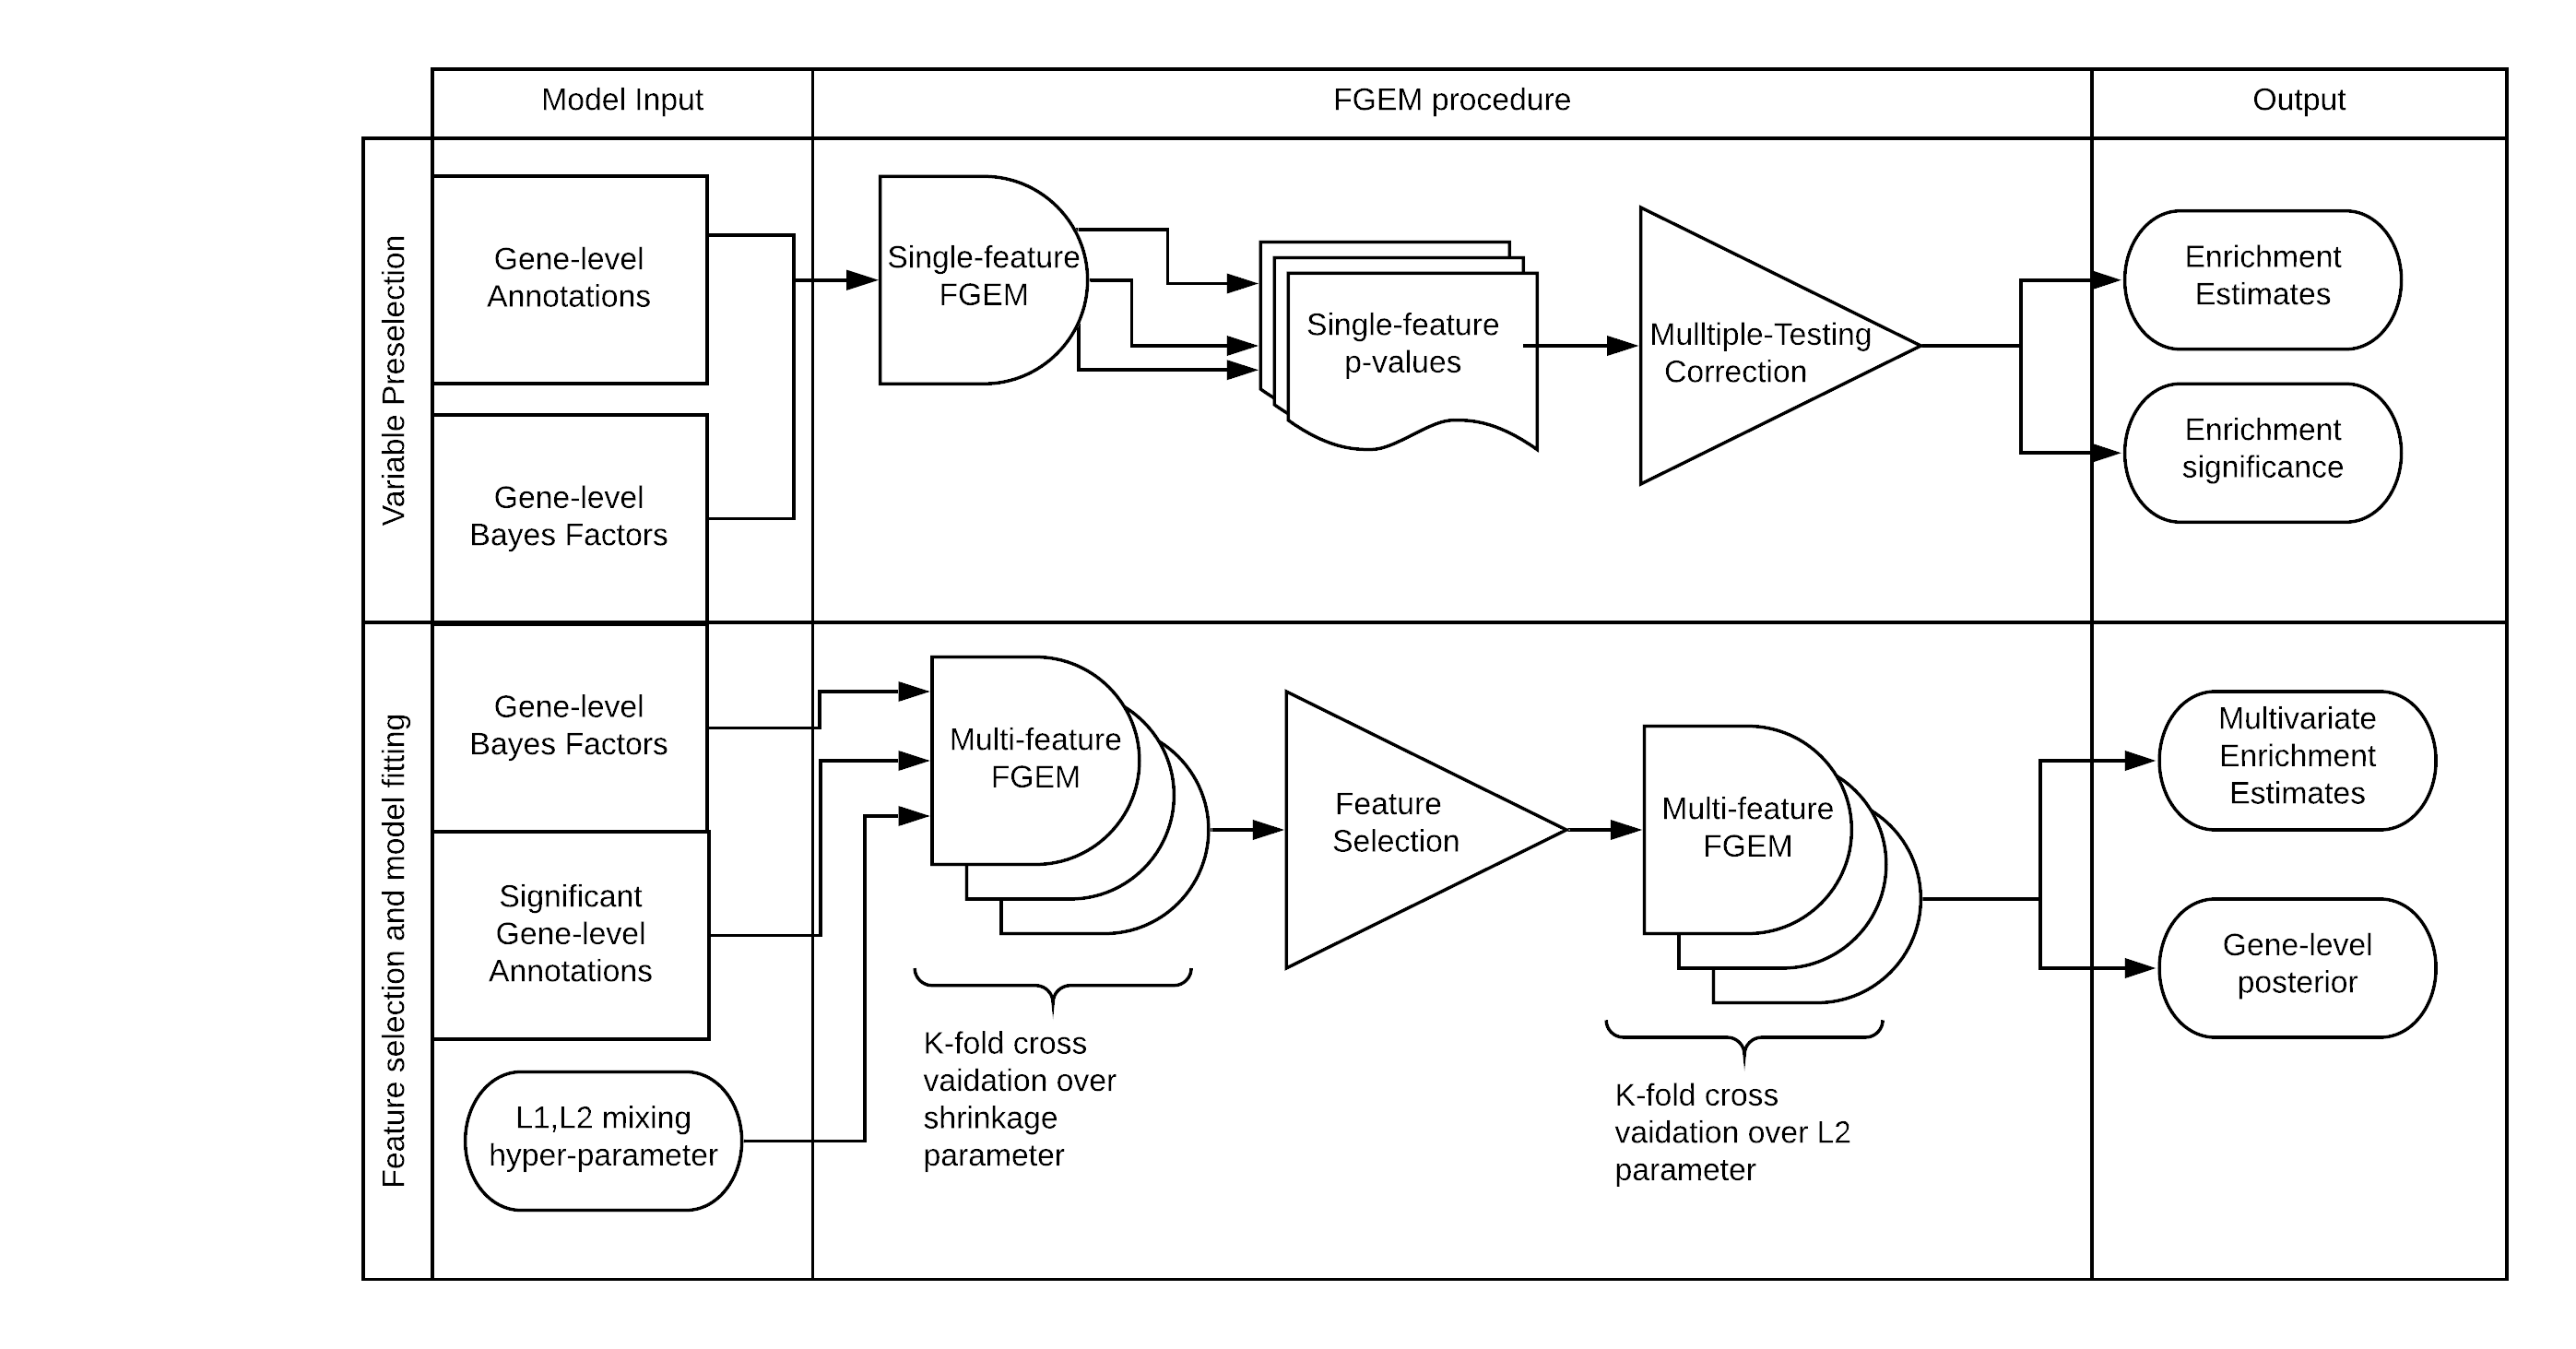
\includegraphics[width=.9\linewidth]{img/FGEM_procedure.png}\label{fig:overview}
  \caption{Overview of the FGEM procedure for gene-set enrichment and gene mapping.  In the preliminary feature pre-selection phase, all single-feature models are fit, and $p$-values are obtained for each model.
    Features with FDR-adjusted $p$-value less than a significance cutoff (0.1) are incorporated in the multivariate model. The multivariate model is fit with an elastic-net penalty, with a user-specified proportion of $l_1$
    to $l_2$ penalty ($\alpha$), and $k$-fold cross-validation to determine the optimal penalty parameter ($\lambda_{\text{opt}}$).  The subset of features with non-zero enrichment estimates under the model with the selected $\lambda_{\text{opt}}$ undergo a final round of $l_2$ only $k$-fold cross-validation (i.e relaxed elastic-net).  The final $l_2$ penalized multivariate enrichment estimates are then used to generate gene-level posteriors. }
\end{figure}


\subsection{A probabilistic framework for gene-set enrichment and gene prioritization applied to cancer gene discovery}\label{sec:org2d4ff20}

Our approach is outlined in\ref{fig:overview}. In brief, we combine gene-level Bayes factors summarizing the hypothesis that a gene is causally related to a trait of interest with gene-level annotations about that gene to simultaneously re-estimate the gene-level posterior probability that the gene is causal and identify the properties causal genes are likely to have.  Let $Z_g$ be and indicator variable with $Z_g = 1$ indicating that gene $g$ is causally related to the trait of interest, and $Z_g = 0$ indicating that it is not.  While $Z_g$ is unobserved, the evidence for and against $Z_g=1$, as calculated by a gene-based test on some body of genetic evidence, is summarized by the Bayes factor forthat gene $B_g$.  FGEM incorporates gene-level annotation, represented as an $F$ (the total number of gene-level features), by $G$ (the total number of genes), matrix $\textbf{A}$, by relating $Z_g$ to $\textbf{A}$ through a length $F$  enrichment parameter $\boldsymbol{\beta}$.  For a particular gene $g$, $P(z_g=1|\textbf{a}_g,\boldsymbol{\beta}) =  \frac{1}{1+e^{-(\beta_{0}+\sum_{f=1}^F{A_{f,g}\beta_f})}} $.  This relationship between feature and and response is
analagous to a logistic regression on a latent variable ($\textbf{Z}$).  The procedure for model fitting is described in the Methods section\ref{sec:org4822ac5}.

Under the univariate FGEM model, in which each feature is considered one at at time, if the value of $\beta$ for a binary gene-level annotation is greater than $0$, this indicates that genes with this annotation have a higher probability of being causally associated with the trait of interest than background genes.  Similarly, an estimate of $0$ indicates that the genes with the feature have the same probability of being causally related to the trait of interest as genes without the annotation.  It is also possible for the estimate of $\beta$ to be less than $0$.  An estimate of less than 0 for a univariate association indicates that the genes with the annotation have a lower probability of causal association than random genes.  The statistical significance of the enrichment estimate of a single feature is assessed using the likelihood ratio test, from which $p$-values were calculated.

For a particular value of $\boldsymbol{\beta}$ (and $\textbf{A}$), we can compute a new expected value for $(Z_g = 1 | \textbf{A},\boldsymbol{\beta})$.
% Under the FGEM model, we model $P(Z_g = 1 | \textbf{A},\boldsymbol{\beta})$.
We refer to the value of $\beta_a$ as the enrichment of feature $a$.  For each of the 18 TCGA cancer types, we fit a univariate for each of the 2,657 Biological Process related GO terms.  We refer to the value of $\beta$ for each feature when fit one at a time as the feature's univariate enrichment.  Significant univariate features for each cancer type were jointly fit for each cancer type.  The estimated value of $\beta$ for each feature under this model is referred to as the multivariate enrichment, and the procedure for obtaining multivariate enrichment estimates is described in the Methods section\ref{sec:orge3a8031}.

\begin{figure}
\centering
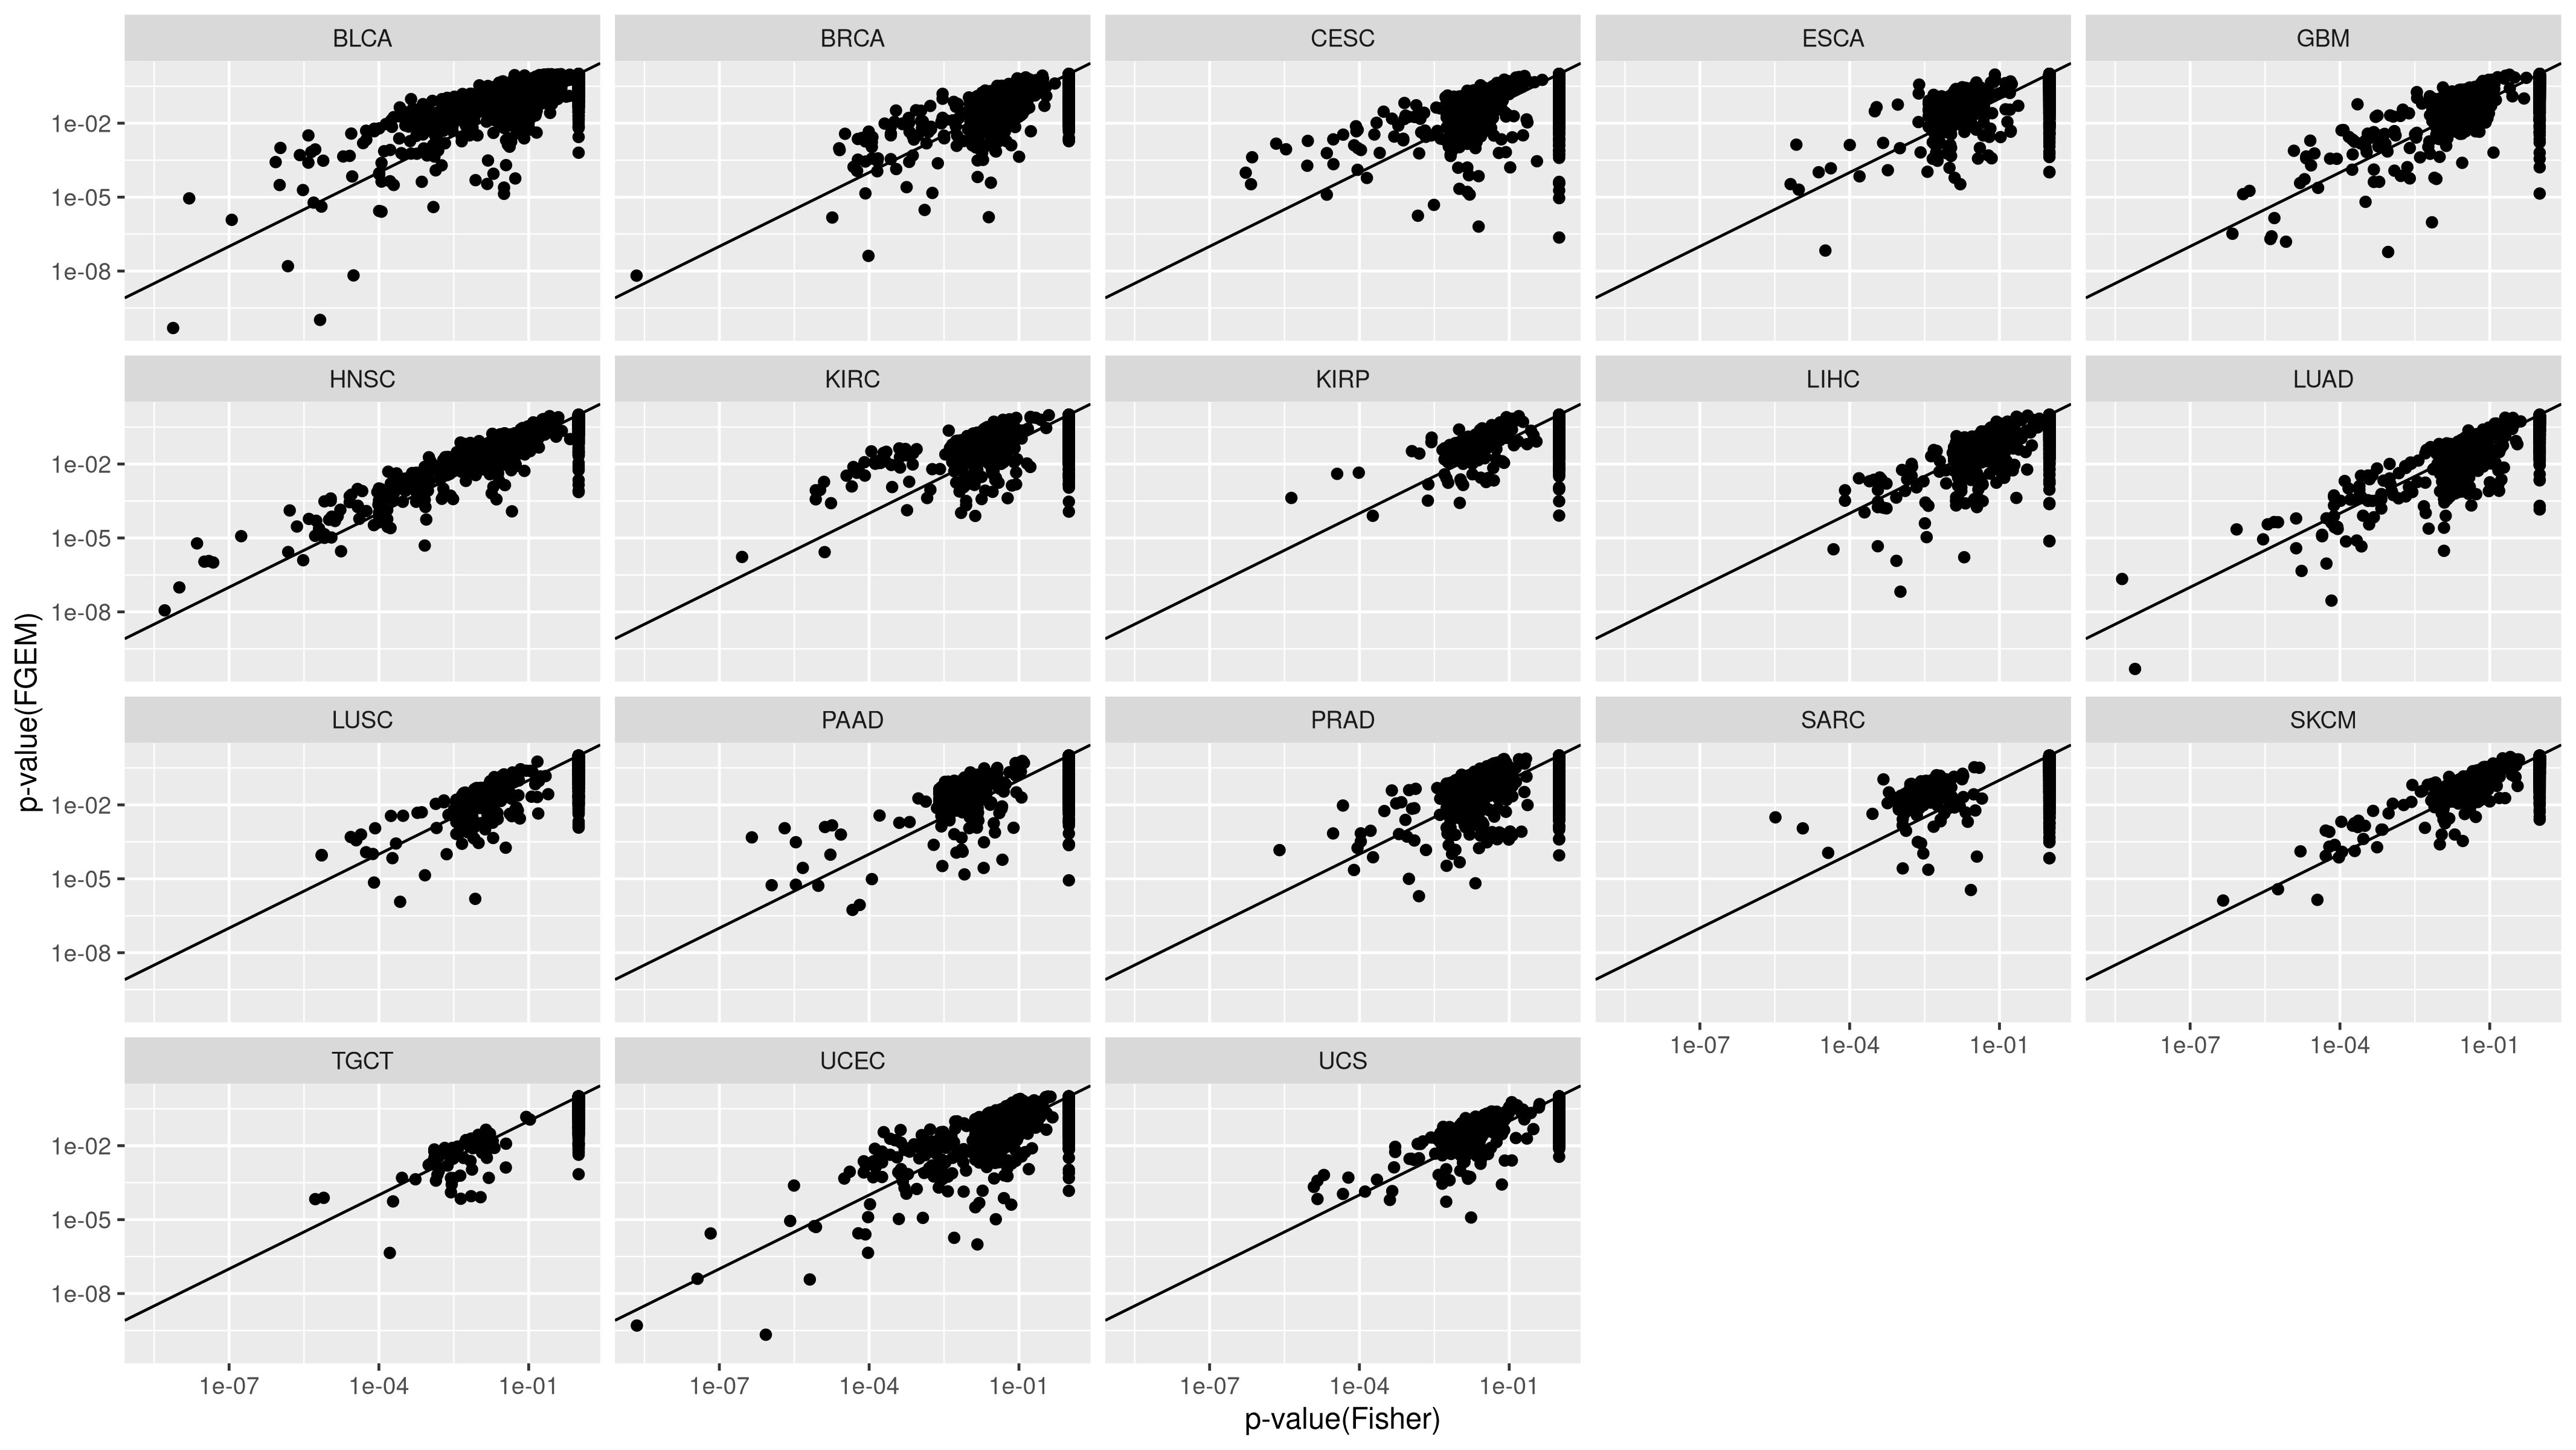
\includegraphics[width=.9\linewidth]{img/fisher_vs_fgem.png}\label{fig:fisher_vs_fgem}
\caption{Comparison of single-feature FGEM and Fisher's exact test $p$-values for 18 TCGA cancer types.}
\end{figure}

\subsection{Recurrent enriched annotations reflect the hallmarks of cancer}\label{sec:orgd52f2ca}

After removing Gene Ontology Biological Process features with a small number of annotated genes, there were 2,657 features.  Evaluating the enrichment of each of these features in a univariate fashion with the 18 TCGA cancer types resulted 47,826 univariate enrichment estimates.  We first evaluated the number of significantly enriched features, stratified by cancer type.  With a false discovery rate (FDR) of $0.01$, all cancer types but KIRP and UCS had at least one (i.e 16 out of 18) significant association, with HNSC having the most, at 38.\ref{tab:univariateFDR}.  With a relaxed FDR of $0.15$, all 18 cancer types had at least one significantly associated feature\ref{tab:univariateFDR}. In all cancer types analyzed, all features with enrichments significantly different from 0 (at all tested FDR) were positively enriched.  


\begin{table}
  \centering
  \begin{tabular}{l|r|r|r|r}
    \hline
    cancer & FDR$=0.01$ & FDR$=0.05$ & FDR=$0.1$ & FDR=$0.2$ \\
    \hline
    HNSC & 38 & 95 & 122 & 209\\
    
    LUAD & 31 & 77 & 111 & 190\\
    
    BLCA & 26 & 51 & 67 & 110\\
    
    UCEC & 22 & 52 & 92 & 141\\
    
    GBM & 20 & 42 & 55 & 99\\
    
    CESC & 14 & 36 & 67 & 115\\
    
    PAAD & 11 & 22 & 32 & 54\\
    
    BRCA & 8 & 26 & 37 & 82\\
    
    LIHC & 8 & 33 & 55 & 95\\
    
    LUSC & 4 & 11 & 24 & 53\\
    
    PRAD & 3 & 15 & 50 & 131\\
    
    SKCM & 3 & 8 & 14 & 26\\
    
    KIRC & 2 & 2 & 14 & 53\\
    
    ESCA & 1 & 13 & 31 & 54\\
    
    SARC & 1 & 8 & 14 & 29\\
    
    TGCT & 1 & 8 & 15 & 27\\
    
    KIRP & 0 & 0 & 0 & 6\\
    
    UCS & 0 & 4 & 20 & 23\\
    
  \end{tabular}\label{tab:univariateFDR}
  \caption{Number of significantly enriched features in univariate enrichment test at four False Discovery Rates.}
\end{table}

Next we identified a set of recurrent features: features that were significantly enriched in more than one cancer type.  We characterized 161 Gene Ontology features as significantly enriched in more than one cancer type, and 50
features were significantly enriched in 5 or more cancer types.  The top features ranked by the number cancer types in which the feature was enriched\ref{tab:sig_univariate} recapitulates almost all of the 10 ``Hallmarks of cancer''
\cite{Hanahan_2011}.  The feature with the higest mean (and median) enrichment is GO:2000774, positive regulation of cellular senescence, with a median enrichment estimate of 5.458, and a mean enrichment estiamte of 7.91.  In a third of cancer types analyzed (6 of the 18), the univarite, FDR-adjusted $p$-value for GO:2000774 was less than 0.1.  The relevance of this feature to cancer is obvious and bordering on tautalogical: mutations in genes that prevent the cell from entering oncogene induced cellular senscence (especially those related to the ARF/TP53 pathway) are thought to be all but essential for progression of almost all cancers\cite{chandeck10_oncog_induc_cellul_senes}.  It is difficult to overstate the importance of positive regulation of cellular senescence as a key guard against cancer.  Indeed, TP53 had the highest average log Bayes Factor of all genes going in to the analysis, and had the highest average posterior probability of being a cancer gene as a result of the analysis, reinforcing the finding that regulators of cellular senescence, and those in the TP53 pathway in particular, are highly enriched for mutational driver genes.

 
\begin{table}[ht]
\centering
\begin{tabular}{lcll}
  \hline
  \thead{GO Term} & \thead{Average $\beta$} & \thead{No. significant} & \thead{Description} \\ 
  \hline
GO:0007265 & 3.28 &  12 & Ras protein signal transduction \\ 
GO:0008285 & 2.29 &  12 & \makecell[l]{negative regulation of\\ cell population proliferation} \\ 
GO:0019221 & 2.63 &  11 & cytokine-mediated signaling pathway \\ 
GO:0010628 & 2.34 &  11 & positive regulation of gene expression \\ 
GO:0032228 & 5.60 &  10 & regulation of synaptic transmission, GABAergic \\ 
GO:0010666 & 4.22 &  10 & \makecell[l]{positive regulation of \\ cardiac muscle cell apoptotic process} \\ 
GO:0051402 & 3.17 &   9 & neuron apoptotic process \\ 
GO:2000134 & 2.94 &   9 & \makecell[l]{negative regulation of G1/S \\ transition of mitotic cell cycle} \\ 
GO:0007050 & 2.51 &   9 & cell cycle arrest \\ 
GO:0045893 & 2.02 &   9 & \makecell[l]{positive regulation of transcription,\\ DNA-templated} \\ 
GO:0043276 & 5.25 &   8 & anoikis \\ 
GO:2000379 & 4.22 &   8 & \makecell[l]{positive regulation of reactive \\ oxygen species metabolic process} \\ 
GO:0043491 & 3.57 &   8 & protein kinase B signaling \\ 
GO:0043542 & 3.07 &   8 & endothelial cell migration \\ 
GO:0000165 & 2.66 &   8 & MAPK cascade \\ 
\end{tabular}\label{tab:sig_univariate}
\caption{Top features of mutational cancer driver genes from single-feature enrichment analysis.  Features are ranked by the number of cancer types in which the feature was significant at (FDR-adjusted) $p \leq 0.1$, and then by the average enrichment estimate among all cancer types.     }
\end{table}


There were two features that were the most recurrent: features with a significant enrichment estimate in the largest number of cancers.  GO:0007265 (Ras protein signal transduction) had a mean univariate estimate of 3.28 (and median of
0.96), had an FDR-adjusted $p$-value of less than 0.1 in three quarters of cancer types analyzed (12 out of 18). In addition to oncogenic Ras having a capacity to endow cells with growth signal sufficiency, oncogenic Ras, and members
of the Ras signaling pathway, have been implicated in several other cancer hallmarks\cite{Pylayeva_Gupta_2011}.  Tied with the Ras signal transduction feature, as the feature which passed the significance threshold in the largest
number of cancers was GO:0008285, negative regulation of cell population proliferation.  Negative regulation of cell population proliferation, like positive regulation of cellular senescence, is key to preventing uncontrolled cell growth; a defining feature of cancer\cite{Hanahan_2011}.

\subsection{FGEM integrates multiple gene-level annotations to selectively reprioritize mutational driver genes}\label{sec:orgf0225be}

A perennial challenge in developing statistical methods for gene mapping is deciding on criteria for validation, as the true status of each gene is often unknown\cite{Schaid_2018}\cite{drivermaps}.  IntOGen is a database of cancer driver genes that is populated by an ensemble method that incorporates seven different methods for identifying mutational driver cancer genes. To check whether FGEM reprioritization improved prediction of mutational cancer driver genes, we compared whether the posterior probability for IntOGen validated cancer genes was higher under the uniform model (intercept only) or the functional model. In every cancer type, validated cancer genes had a higher posterior under the functional model as compared to the uniform model;  genes that were not previously identified as cancer genes in IntOGen had on average lower functional posterior compared to uniform.


\subsubsection{FGEM prioritizes known cancer driver genes that don't accumulate single nucleotide point mutations}

After validating that FGEM improves the power to detect mutational driver genes we turned our attention to which genes increased the most as a consequence of the functional prior.  The gene with the largest average increase in posterior probability between the functional and uniform posterior  was the gene for  Transforming Growth Factor Beta 1, or TGFB1.  The posterior for TGFB1 increased by an average of 0.496, with a median increase of 0.417.  In 18 of the 20 cancers for which \texttt{driverMAPS} data is available, the log Bayes factor for TGFB1 is negative, and in the 2 cases where it is positive (UCS and SARC), the log Bayes factors are 0.912 and 0.661, which is well below any reasonable threshold one might warrant for further investigation.  While TGFB1 is not characterized by intogen as a mutational cancer driver (due to the relatively lower number of somatic point mutations observed in tumors),  the role of TGFB1 in metastasis, and the role of the TGF-$\beta$ signaling pathway more generally in cancer progression is widely known and studied\cite{TGF_Zhao_2018}.  While TGFB1 may not accumulate point mutations at a significantly higher rate than background mutational processes suggest, the carcinogenic consequences of upregulation through amplification or trans-acting gene-regulatory means have been well documented\cite{TGF_Zhao_2018}\cite{Massagu__2008}.
After TGFB1, the gene with the largest increase in posterior probability that is not a known mutational cancer driver is JUN.  JUN is the gene with the highest minimal increase in posterior probability.  JUN increased in posterior over the uniform model in every cancer in which it was tested, and by at least 0.01.  Only 3 genes increased in posterior probability over the uniform model in every cancer type (the aforementioned JUN, IGF1 and KRAS). While JUN is not a known mutational cancer driver gene according to intogen, a brief literature review reveals that not only is JUN a known mutational cancer driver gene, but that JUN was the first oncogenic transcription factor ever discovered, but was initially discovered as a viral oncogene\cite{Vogt_2002}.  

Across all analyses, the gene with the single largest increase in posterior probability was in SKCM, where cyclin-dependent kinase inhibitor 1, or CDKN1A, which while having a log Bayes factor of only -0.10, had a posterior probability under the uniform of 0.005, but a posterior under the functional model of 0.979.  The prior probability of CDKN1A being a driver gene according to the multivariate model in SKCM was 0.98.  The high prior for CDKN1A was driven by the 8 GO terms with non-zero enrichment estimates associated with CDKN1A (see table\ref{tab:CDKN1A_features}).  CDKN1A, which is also known as p21 is a regulator of cell cycle at G1, and the expression of CDKN1A is known to be tightly controlled by the tumor suppressor p53, but it is also hypothesized to have p53 independent tumor suppressor activites\cite{abbas09_p21_cancer}.  CDKN1A has not been previously identified as a mutational driver gene in the intogen database in the context of melanoma, though it has been identified in bladder cancer, hepatic cancer, and chromophobe renal cell carcinoma\cite{gonzalez-perez13_intog_mutat_ident_cancer_driver}.  However, in a study of expression of CDKN1A in primary and metastatic melanomas as compared to benign lesions, both primary and metastatic melanomas showed higher expression of CDKN1A as compared to benign lesions\cite{Trotter_1997}.  Furthermore, a study in a mouse model of melanoma found that inhibition of CDKN1A and CDKN2C significantly increased the effectiveness of BRAF inhibitors in reducing tumor volume\cite{Jalili_2012}.  


\begin{figure}
  \centering
  \begin{tabular}{l|r|l}
    \hline
    GO term & Beta & Description\\
    \hline
    GO:0007265 & 1.7815778 & Ras protein signal transduction\\
    \hline
    GO:0090398 & 1.3806284 & cellular senescence\\
    \hline
    GO:0030308 & 1.3785728 & negative regulation of cell growth\\
    \hline
    GO:2000134 & 1.3079475 & negative regulation of G1/S transition of mitotic cell cycle\\
    \hline
    GO:0000082 & 0.7519148 & G1/S transition of mitotic cell cycle\\
    \hline
    GO:0007050 & 0.5329066 & cell cycle arrest\\
    \hline
    GO:0090399 & 0.4994682 & replicative senescence\\
    \hline
    GO:0045736 & 0.3218208 & negative regulation of cyclin-dependent protein serine \\
            & & threonine kinase activity\\
    \hline
  \end{tabular}\label{tab:CDKN1A_features}
  \caption{Multivariate estimates of enrichment of CDKN1A-related GO-terms in SKCM.}
\end{figure}

\begin{figure}
    \centering
    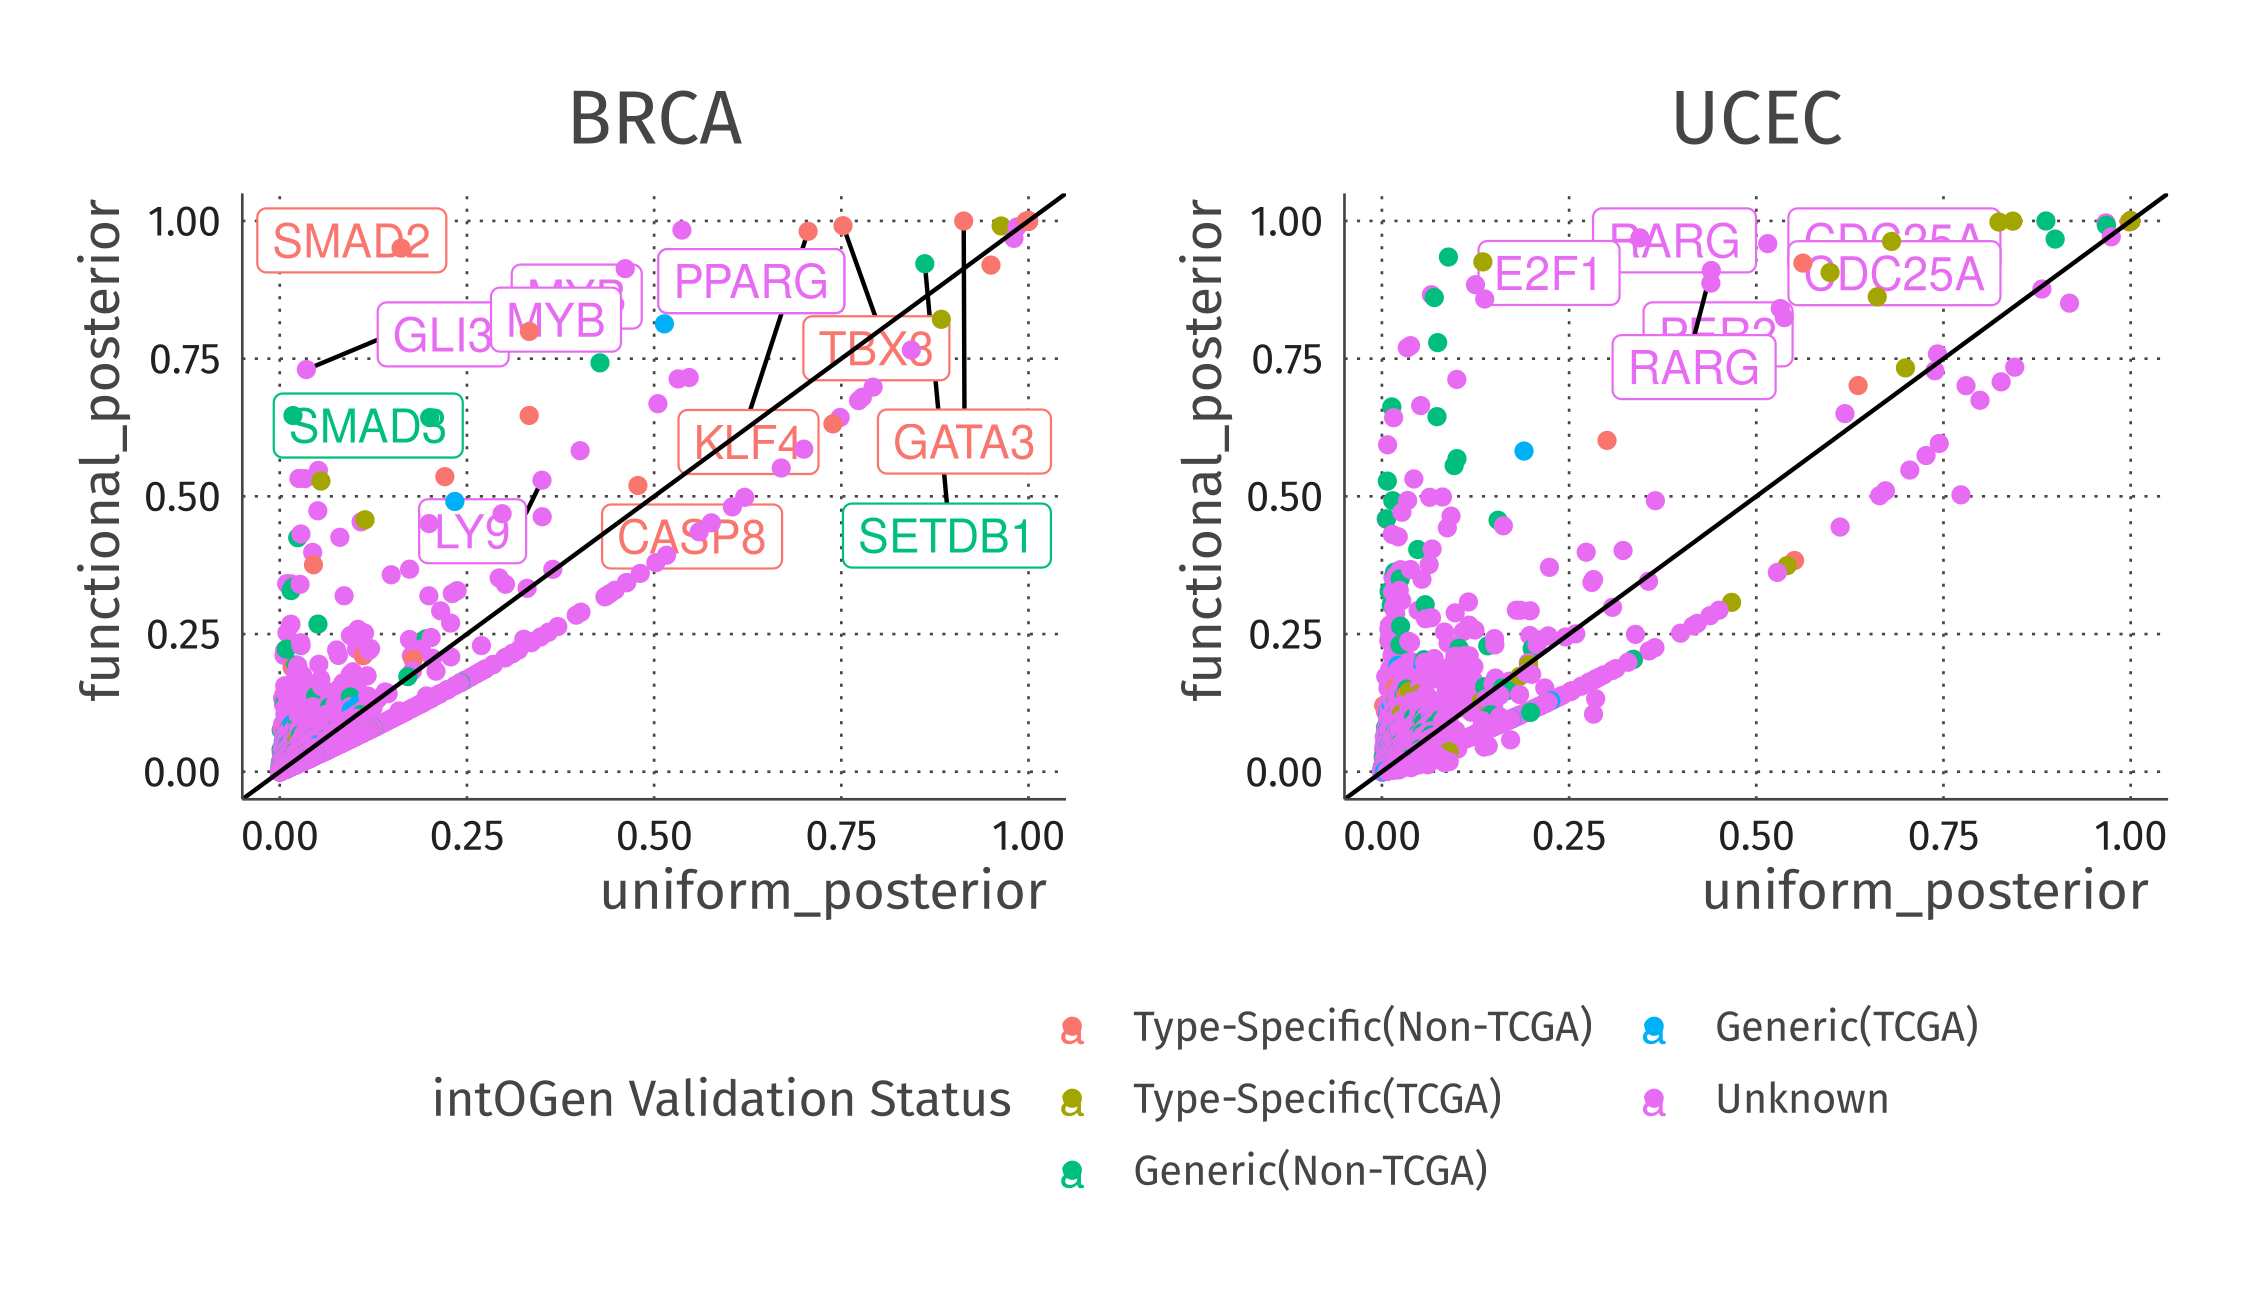
\includegraphics[width=.9\linewidth]{img/fgem_posterior_plot.png}\label{fig:fgem_posterior}
    \caption{Comparison of gene-level posterior under uniform and functional models for  Breast Invasive Carcinoma (BRCA) and Uterine Corpus Endometrial Carcinoma (UCEC).}
\end{figure}

\begin{figure}
    \centering
    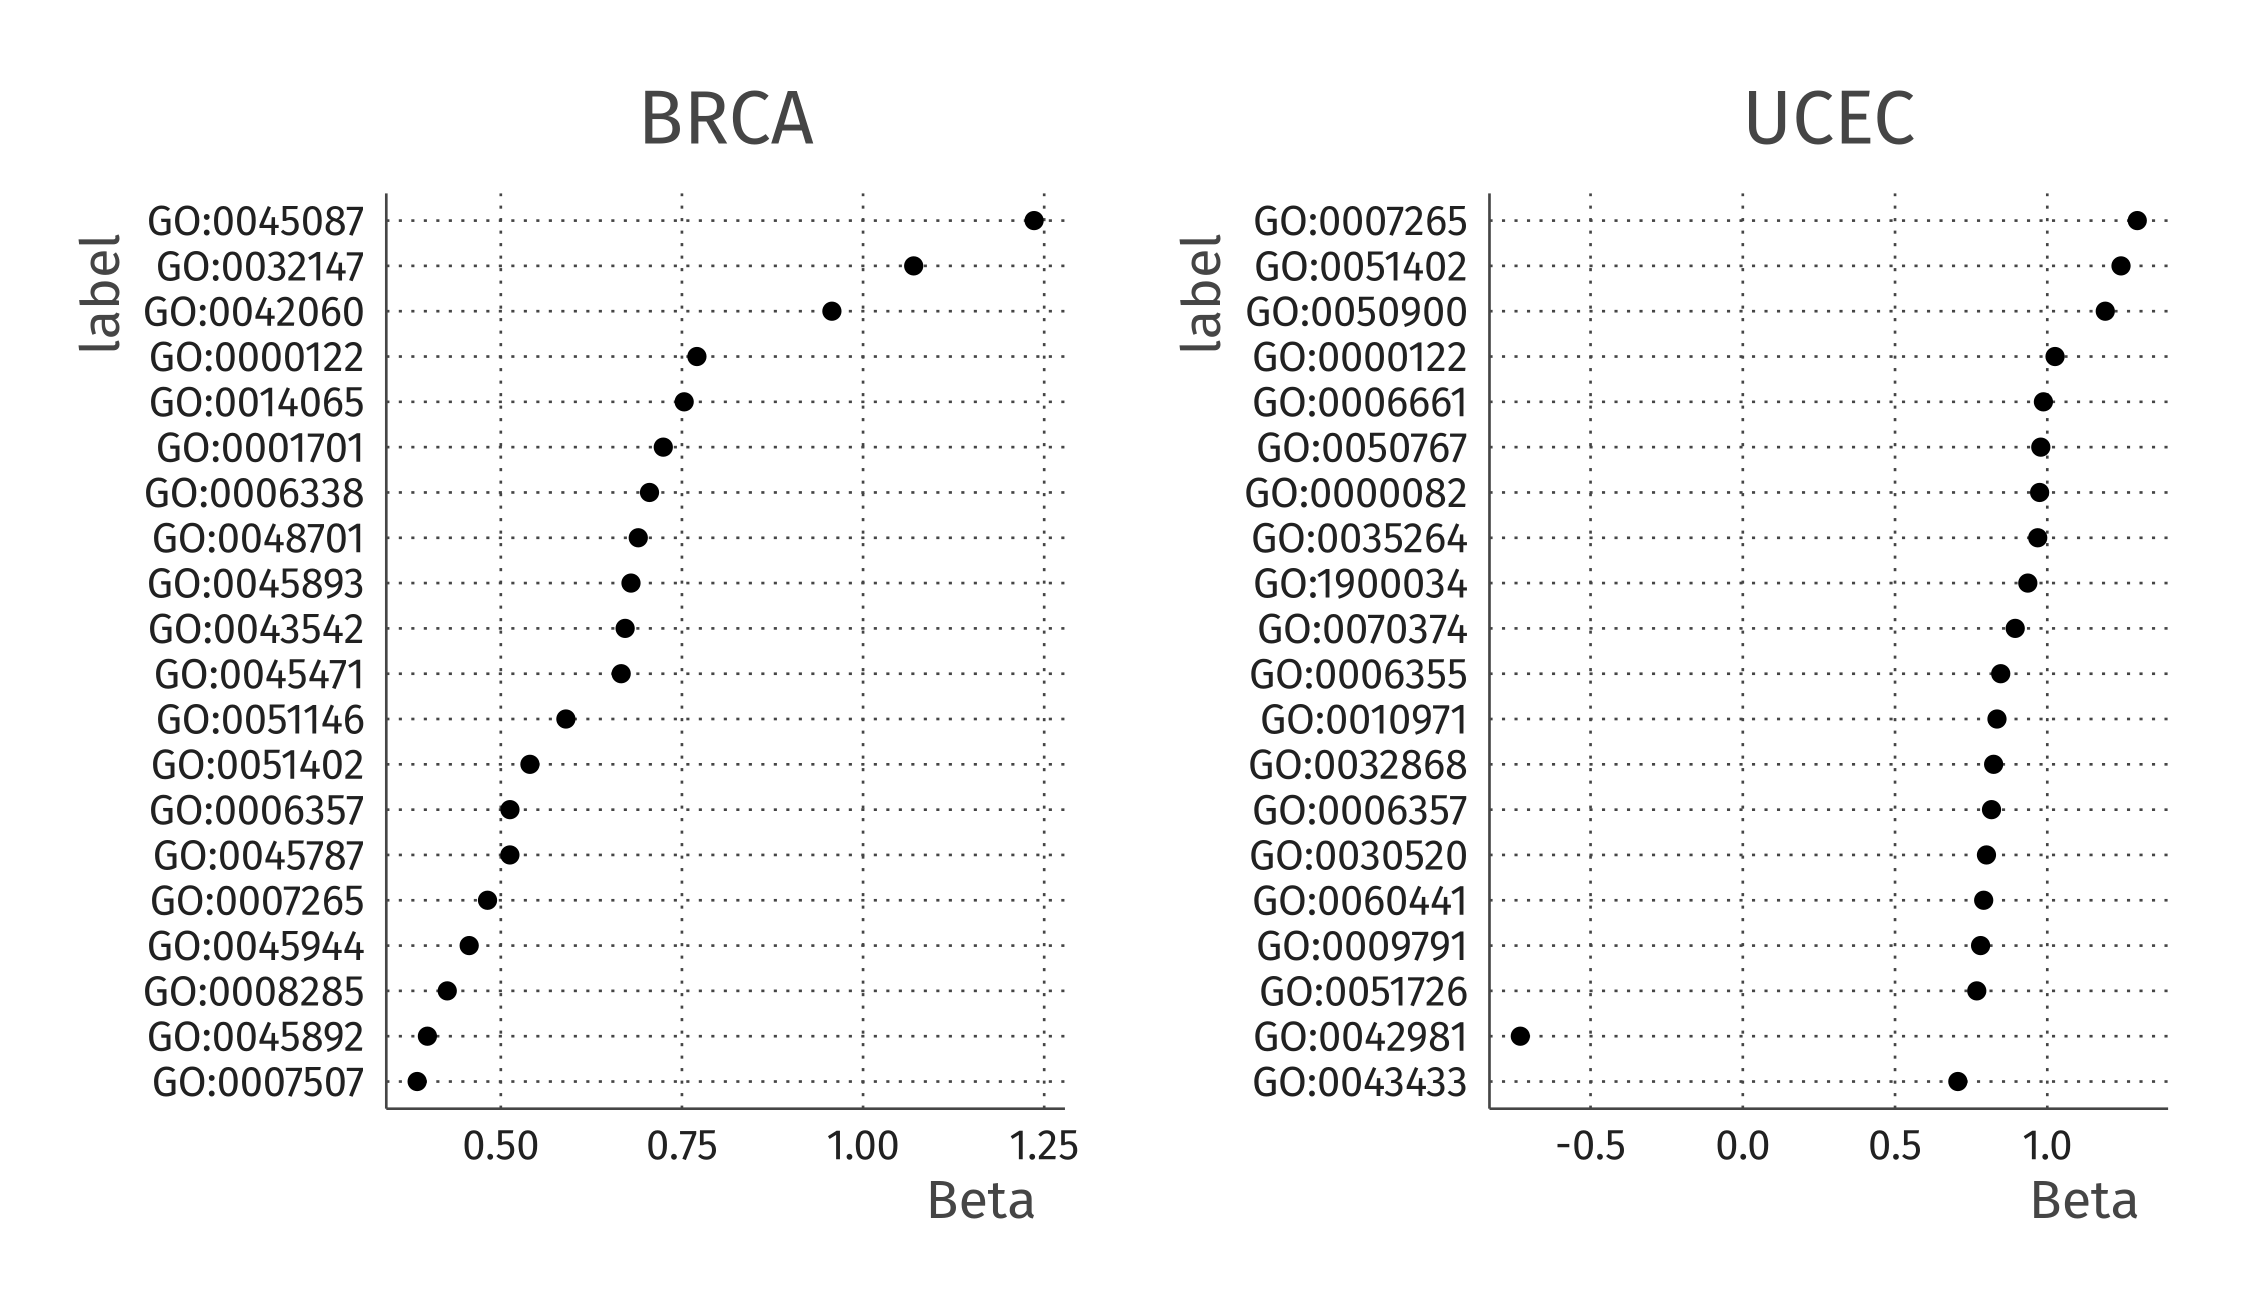
\includegraphics[width=.9\linewidth]{img/fgem_enrichment_plot.png}
    \caption{Multivariate enrichment estimate of the top 20 features (by absolute enrichment) for BRCA and UCEC.} 
\end{figure}



\begin{figure}
    \centering
\begin{tabular}{l|l|r|r|r|r|l}
\hline
Cancer & Gene & BF & functional posterior & uniform posterior & functional prior & intOGen Validation Status\\
\hline
SKCM & CDKN1A & -0.1050424 & 0.9785335 & 0.0051083 & 0.9806326 & Known \\
\hline
PRAD & SMAD3 & 0.0166564 & 0.9914754 & 0.0196157 & 0.9913334 & Known \\
\hline
PAAD & BMP2 & -0.2161379 & 0.9894372 & 0.0230885 & 0.9914728 & Unknown \\
\hline
KIRC & TGFB1 & -0.4437373 & 0.9721332 & 0.0102885 & 0.9819394 & Unknown \\
\hline
LUAD & PTEN & 1.8961662 & 0.9894831 & 0.0364872 & 0.9338898 & Known \\
\hline
SARC & PTPRK & 0.9053713 & 0.9809541 & 0.0368396 & 0.9541875 & Known \\
\hline
GBM & TGFB1 & -0.3837212 & 0.9467147 & 0.0135079 & 0.9630685 & Unknown \\
\hline
LUSC & FBXW7 & 3.1761937 & 0.9820268 & 0.0953494 & 0.6952001 & Known Type-Specific\\
\hline
UCS & PARK7 & -0.0922800 & 0.8960789 & 0.0129180 & 0.9043635 & Unknown \\
\hline
CESC & AKT1 & 2.0105368 & 0.9891738 & 0.1181437 & 0.9244469 & Known Type-Specific \\
\hline
ESCA & SMARCA2 & 1.3002554 & 0.9106001 & 0.0587907 & 0.7351145 & Unknown \\
\hline
UCEC & PIK3CB & 1.6707522 & 0.9344572 & 0.0888288 & 0.7283980 & Known \\
\hline
LIHC & CDKN1A & 2.7626673 & 0.9893290 & 0.1619111 & 0.8540635 & Known Type-Specific \\
\hline
BRCA & SMAD2 & 2.5716367 & 0.9506715 & 0.1620579 & 0.5955677 & Known Type-Specific \\
\hline
BLCA & PPARG & 1.8800425 & 0.9218300 & 0.1442086 & 0.6427759 & Unknown \\
\hline
KIRP & MAPK1 & 0.3788399 & 0.5871487 & 0.0183591 & 0.4933381 & Known \\
\hline
TGCT & RAC1 & 3.9860580 & 0.7388052 & 0.1906034 & 0.0499121 & Known \\
\hline
\end{tabular}\label{tab:top_inc_genes}
\caption{The gene with the highest increase in posterior probability in each cancer type, along with the status of the gene in the cancer-type specific intogen database\cite{gonzalez-perez13_intog_mutat_ident_cancer_driver}}
\end{figure}




\subsection{Highly enriched single features}\label{sec:org530c0fc}

As stated in the Methods section, Features which corresponded to posterior probabilities in excess of 0.3 were excluded from consideration for inclusion in the joint model.  One consequence of FGEM's latent variable approach
is that it is possible to encounter a scenario analogous to the ``separation'' problem in logistic regression.  In logistic regression, if one (or several) predictors predict an output perfectly, the likelihood for that 
feature is not maximized at a finite parameter value, which can result in extremely high enrichment estimates.  Because there is a high level of redundancy in the Gene Ontology feature-set, little information is lost by excluding these problematic features.  

Overall there were 233 of the 12,019 GO terms across the 18 cancer types which were excluded from the multivariate model due to very high enrichment.  There were several features that were excluded from a large number of cancer types, and several features that had very high average enrichment estimates

The feature with the highest significant enrichment estimate across all cancer types was GO:0045747, positive regulation of Notch signaling pathway, in TGCT.  GO:0045747 had a univariate effect estimate of 7.412 and an FDR-adjusted $p$-value of 0.033.  Notch signaling is known to play an important role in germ cell devlopment and spermatogenesis\cite{Huang_2013}, and TGCT are widely believed to originate from human primordial germ cells\cite{baroni19_origin_testic_germ_cell_tumor}.  The relationship between Notch signaling and TGCT pathogenesis has been explored previously\cite{hayashi04_expres_failur_notch_signal_system}.

\begin{figure}
    \centering
\begin{tabular}{l|r}
  \hline
  Cancer Type & Number of highly enriched features\\
  \hline
  CESC & 43\\
  \hline
  PRAD & 42\\
  \hline
  UCEC & 34\\
  \hline
  GBM & 31\\
  \hline
  LIHC & 30\\
  \hline
  BLCA & 23\\
  \hline
  HNSC & 23\\
  \hline
  KIRC & 22\\
  \hline
  ESCA & 21\\
  \hline
  PAAD & 20\\
  \hline
  BRCA & 19\\
  \hline
  LUAD & 11\\
  \hline
  SARC & 10\\
  \hline
  LUSC & 9\\
  \hline
  TGCT & 6\\
  \hline
  UCS & 6\\
  \hline
  SKCM & 3\\
  \hline
  KIRP & 1\\
  \hline
\end{tabular}\label{fig:n_enriched}
    \caption{The number of features in each cancer type deemed ineligible for inclusion in the multivariate enrichment method due to very high univariate enrichment.}
\end{figure}


\section{Discussion}\label{sec:org3165b14}

We have developed a statistical model for integrating gene-level Bayes factors with gene-level annotations to simultaneously reprioritize the genes and estimate the enrichment of the features. In our analysis of gene-level Bayes factors generated from \texttt{driverMAPS} run on TCGA data, we find that the addition of gene-level features pushes 208 genes previously below a statistical signifiance threshold be novel driver genes across 18 cancer types.
One of the most salient features of FGEM as compared to other enrichment methods like Fisher's Exact test is that FGEM does not binarize data into significant vs insignificant.  For a particular gene set in a particular data set, the enrichment of Fisher's exact test is determined by the cardinality of the entries in the 2 by 2 contingency table.  In the case of Bayes factors, under Fisher's exact test, genes for which the evidence is \emph{in favor} of the null hypothesis is treated identically to genes for which the evidence is \emph{in favor} of the alternative hypothesis, but slightly below the significance cutoff. 

That the previously identified oncogenes JUN and TGFB1 showed a much high posterior probability under the functional model than the uniform models, and that these genes were not previously identified in intOGen demonstrates the value that a method capable of comprehensive integration of all forms of somatic mutation might provide in identifying cancer genes.  Both JUN and TGFB1 rely on mechanisms other than accumulation of point mutation to operate as oncogenes.  As a consequence, they will be missed by methods that rely exclusively on somatic point mutation.
It should be noted that although the FGEM analysis employed for this paper used binary gene-level features, there is nothing inherent in the method precluding inclusion of categorical or even continuous annotations.  For categorical variables (e.g encoding which, of several possible tissues, a gene is known to be expressed in) this would be
trivial: by using a reference level\cite{chambers1992statistical} and a treatment encoding (an additional indicator variable for $k-1$ of the categorical variable's $k$ levels, with the $k$th level being an implicit reference level), the enrichment estimates would have the same interpretation as log odds ratios over the ``intercept'' model.

One important caveat of the FGEM model is that it does not account for errors or uncertainty in the gene-level annotations.  While the Gene Ontology has a formal process for gene annotation, as well as a controlled vocabulary for describing the evidence underlying every gene-annotation pair, this is not true of most gene-level annotations, and even if it were, it is not clear how one might incorporate this evidence.  It is also worth considering the extent to which publication bias, or the ``file-drawer effect'' might contribute to systematic errors in gene-level annotation. It is impossible to know the number of genes that have been tested for a particular biological process or molecular function.  Gene Ontology maintains a blacklist of disallowed gene-feature relationships\cite{huntley14_under_how_why_gene_ontol}, but it captures only the most commonly misreported gene-feature relationships.  Binary gene-level annotation of a GO term ablates the distinction between a gene that has not been assessed for a particular biological process and a gene for which there is strong evidence \emph{against} it being involved in the process.


\begin{figure}
    \centering
    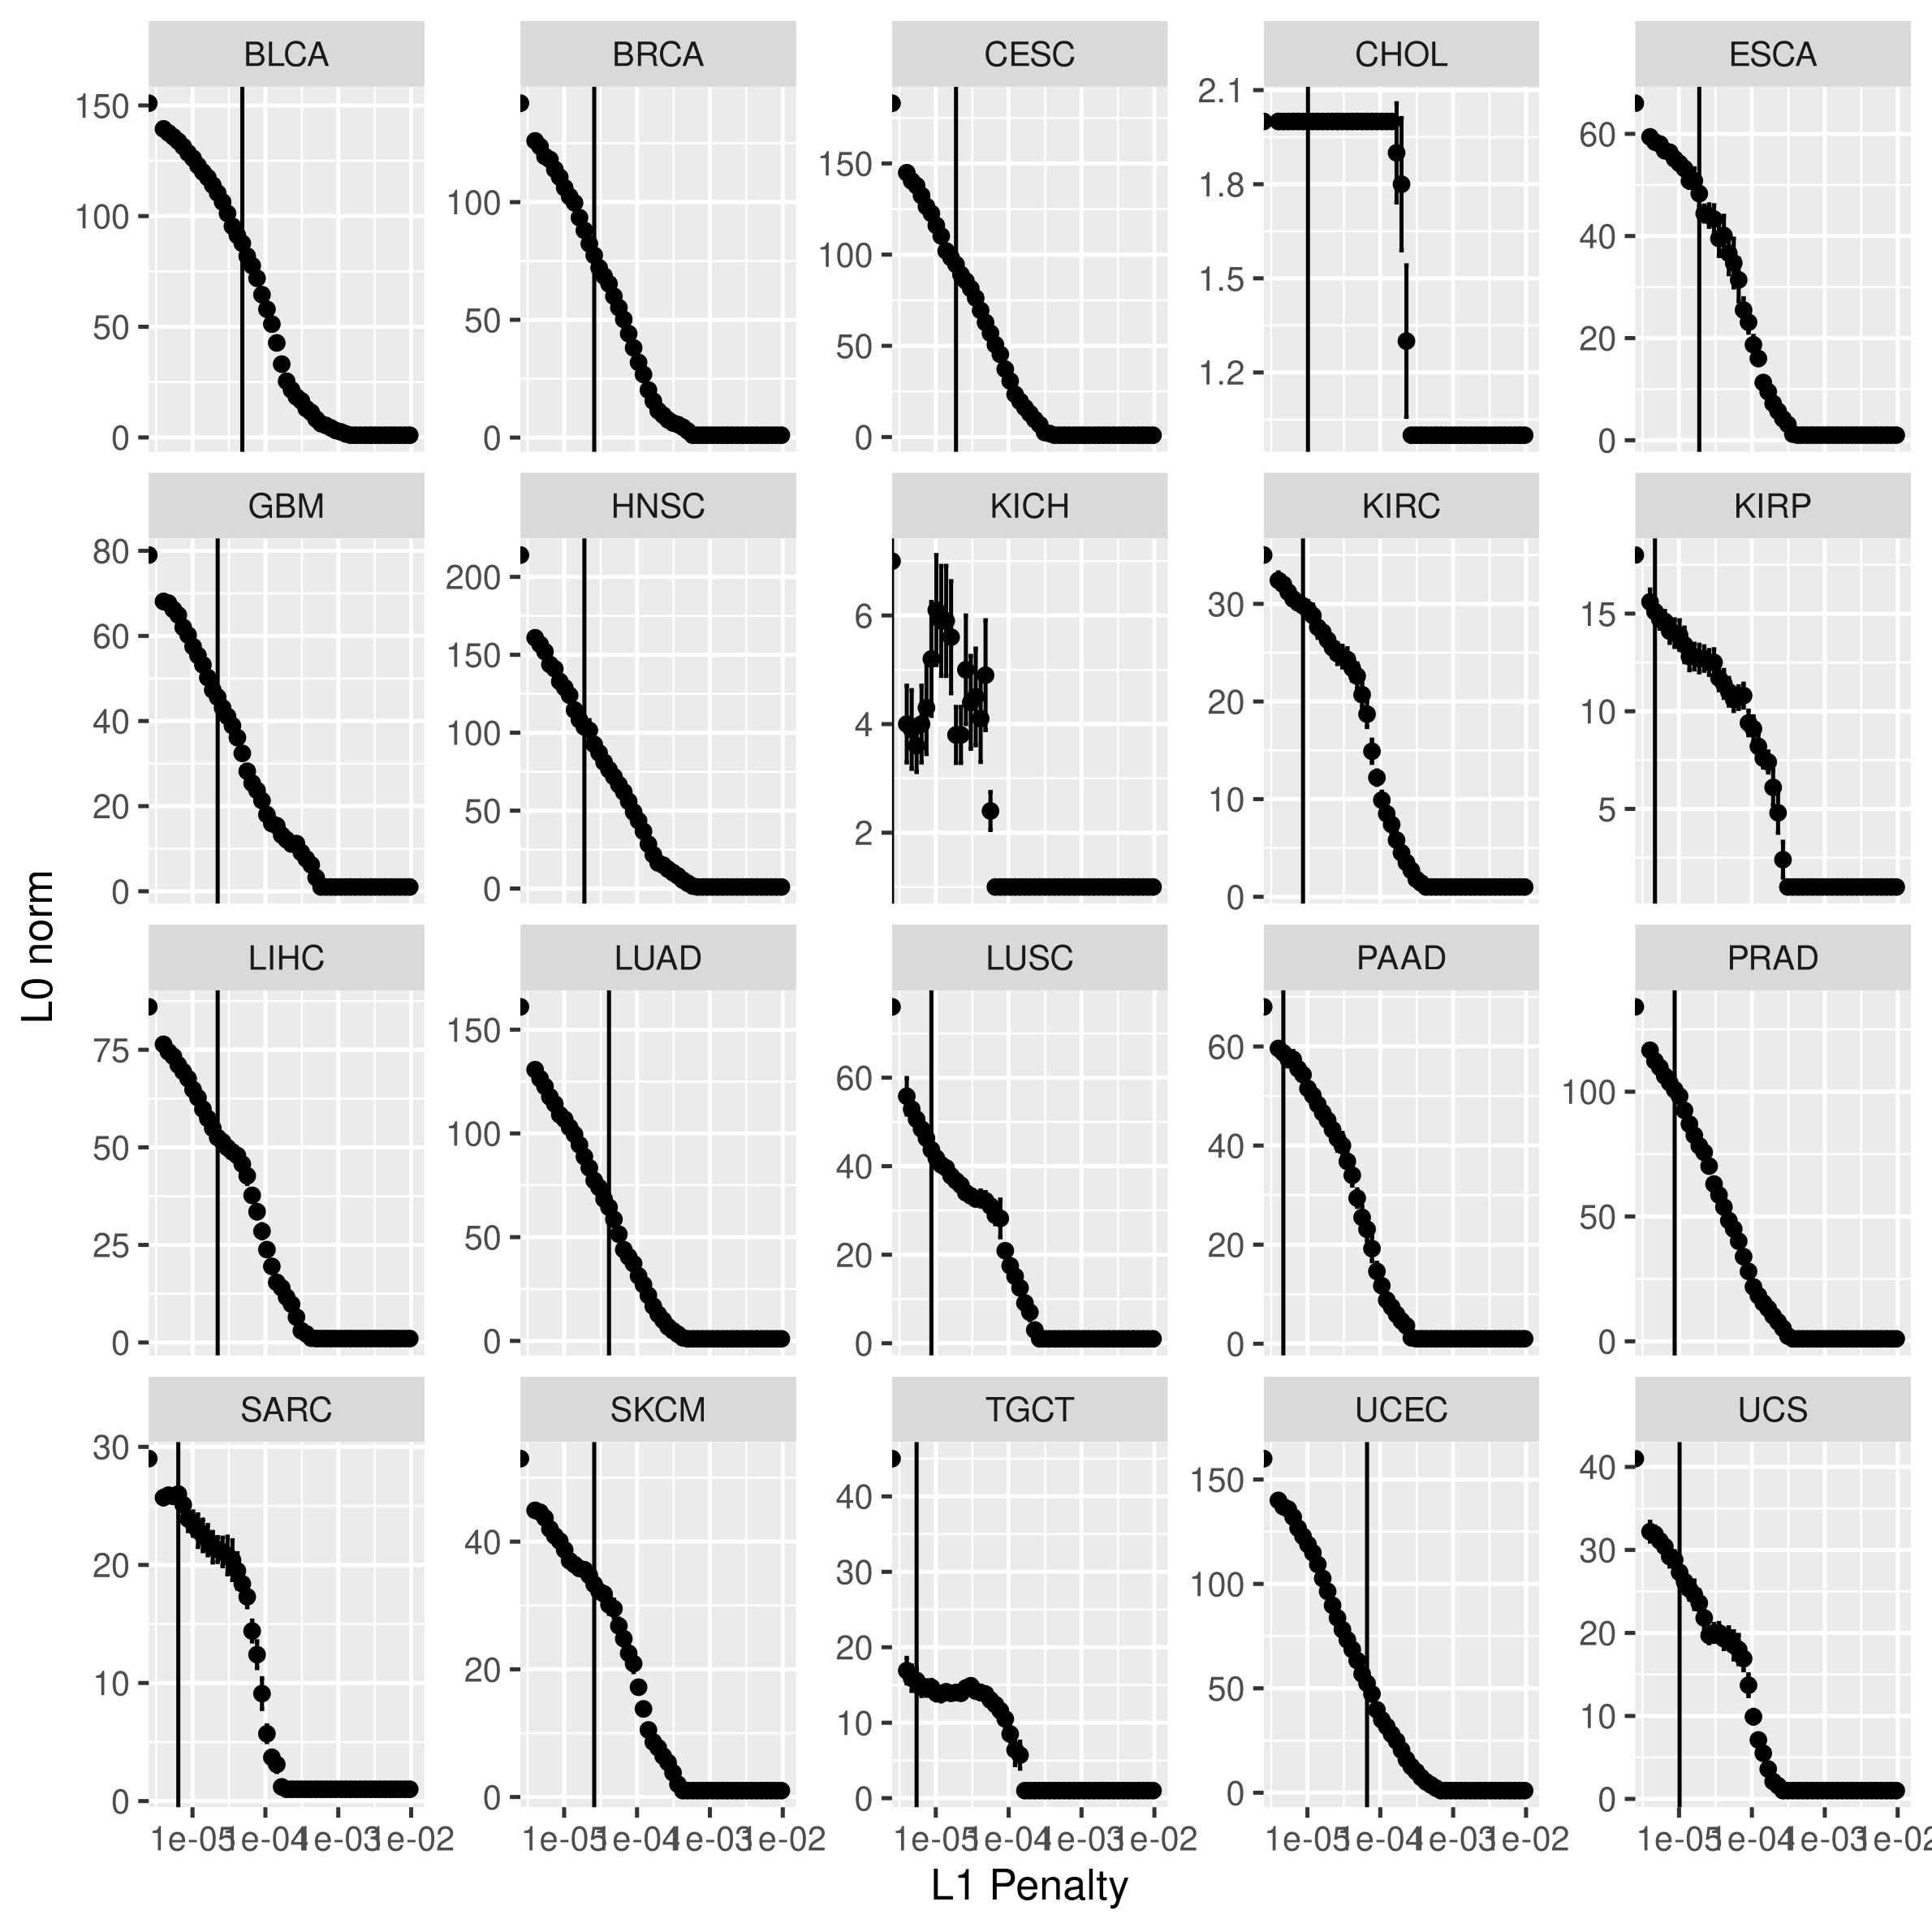
\includegraphics[width=.9\linewidth]{img/cv_l0.png}
    \label{fig:cv_l0}
    \caption{Average (over 10-fold cross-validation) number of features with non-zero effect-size estimates, as a function of $\lambda$, the elastic-net penalty, for each of 18 cancer types.}
\end{figure}

\begin{figure}
    \centering
    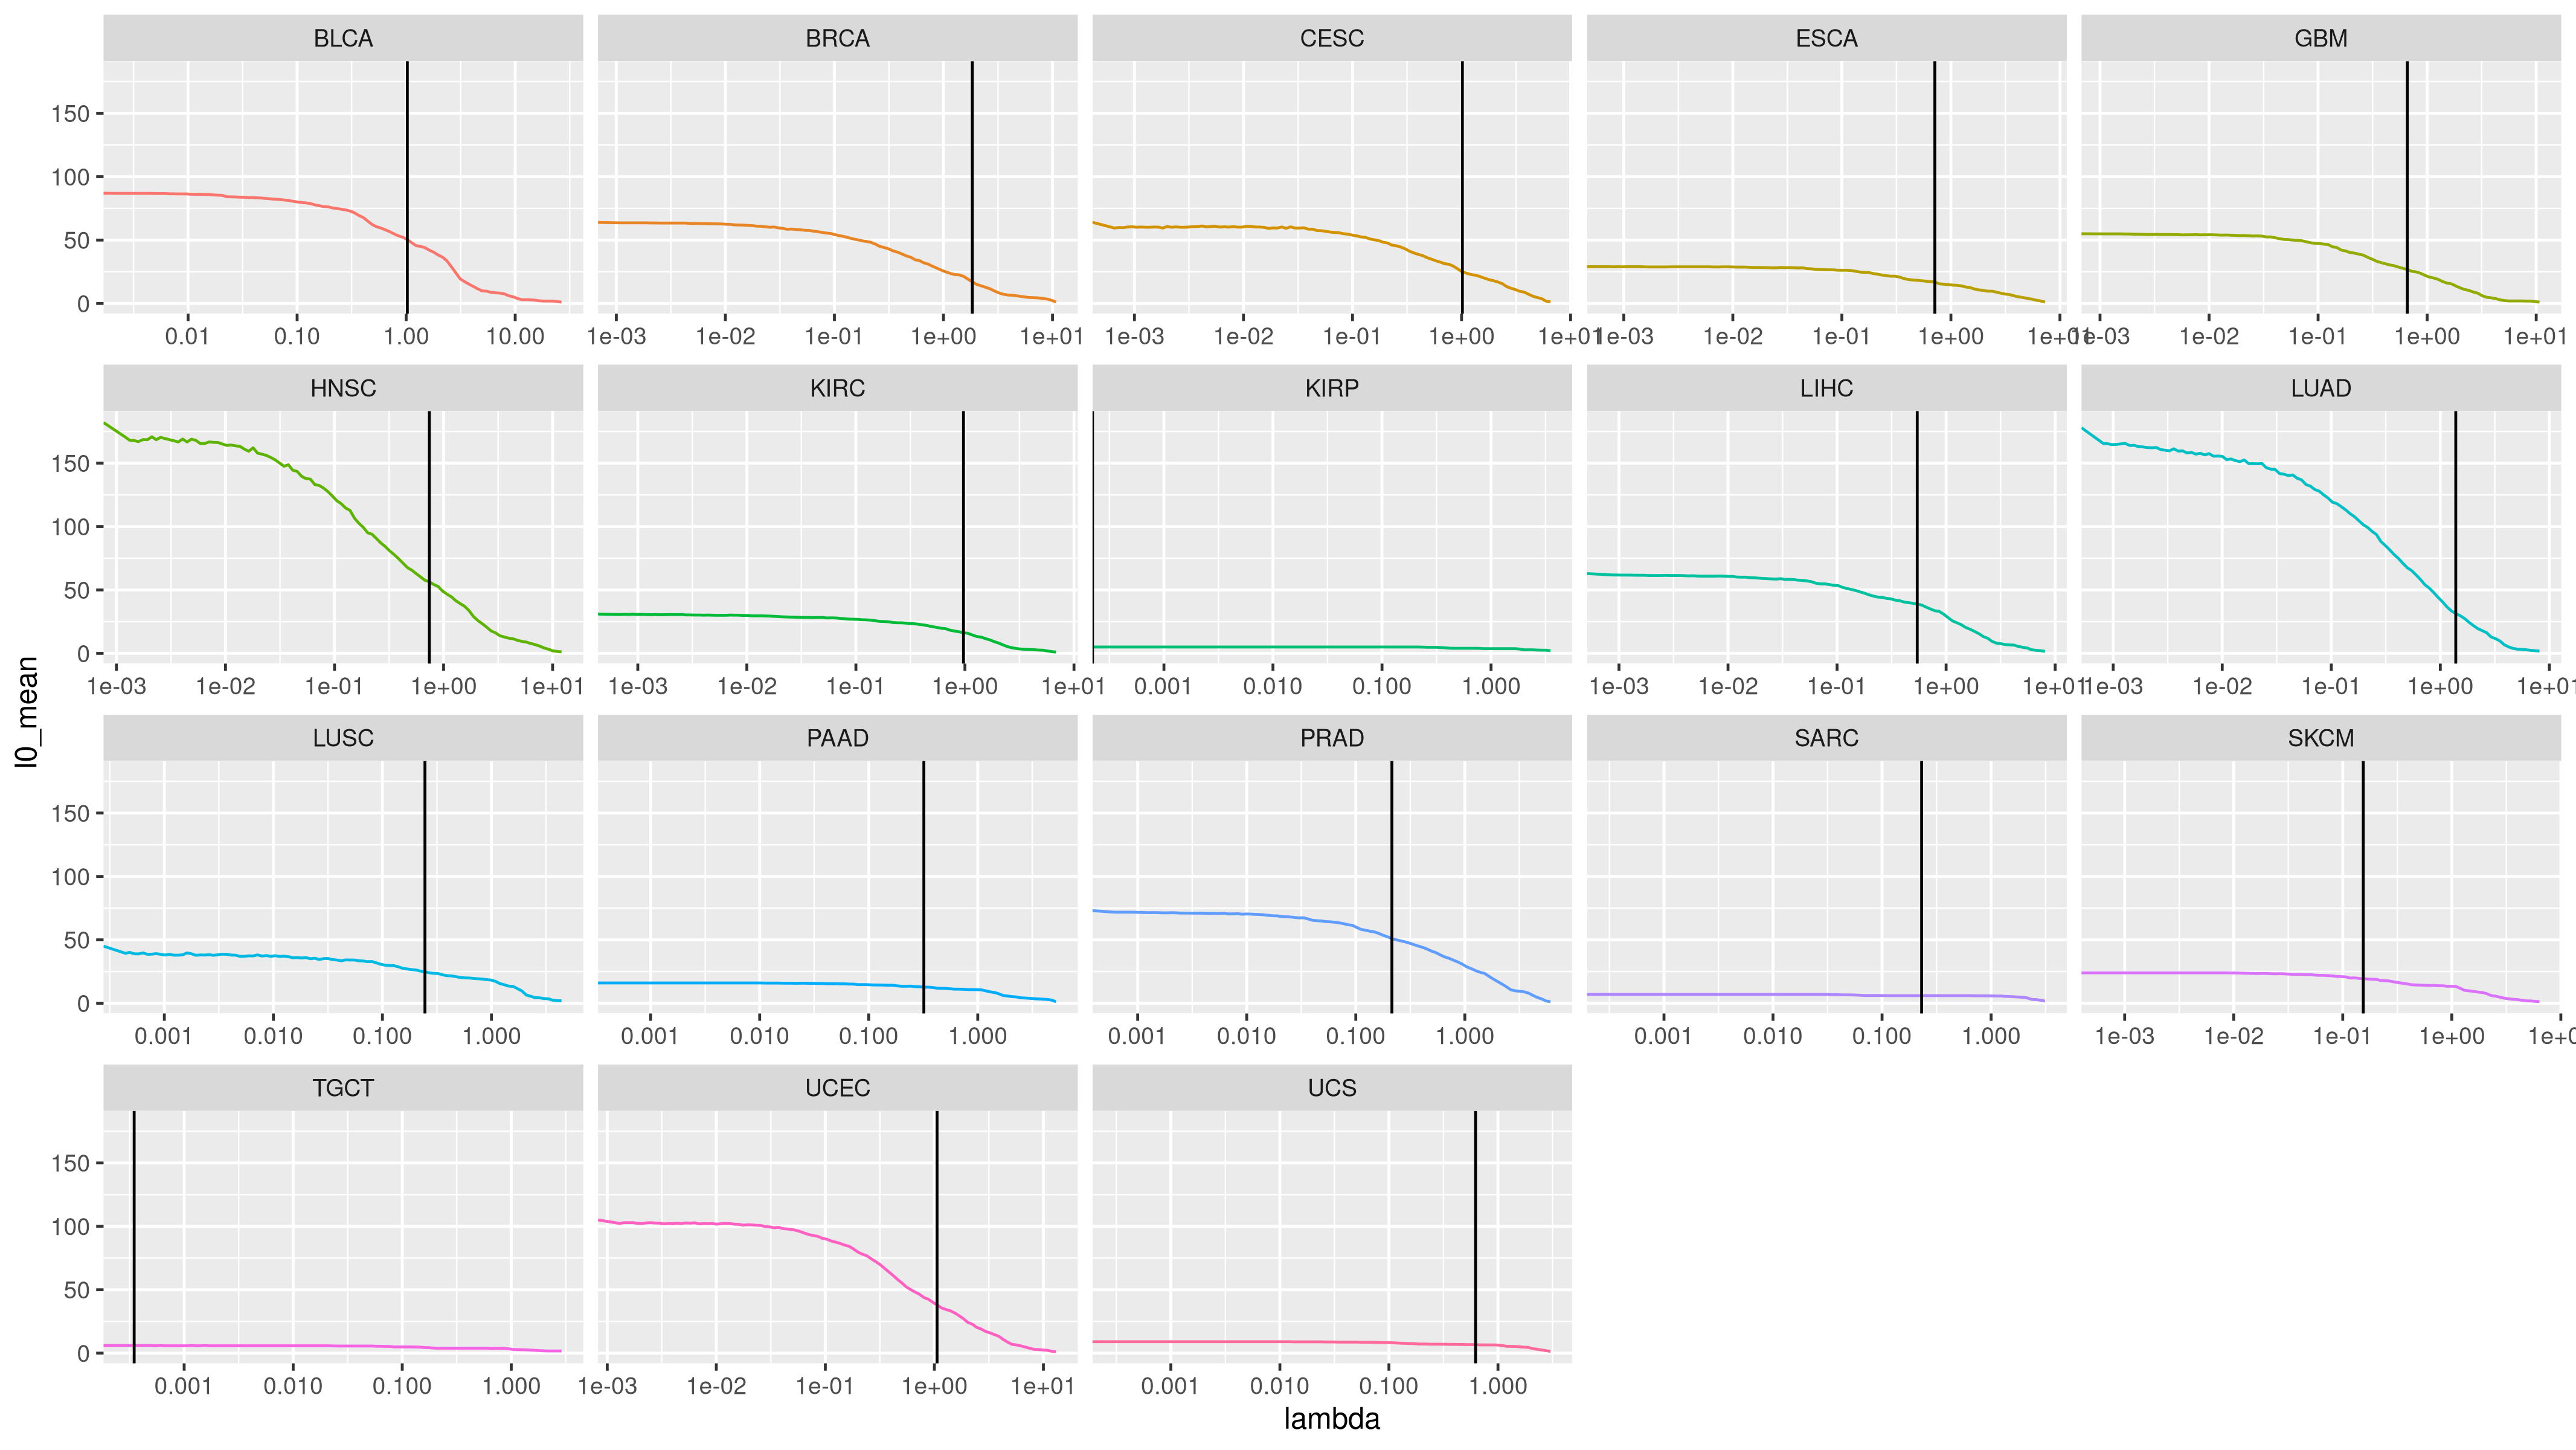
\includegraphics[width=.9\linewidth]{img/enet_cv_l0.png}
    \label{fig:enet_cv_l0}
    \caption{Average (over 10-fold cross-validation) number of features with non-zero effect-size estimates, as a function of $\lambda$, the elastic-net penalty, for each of 18 cancer types.  The vertical line
    represents the optimal value of $\lambda$.}
\end{figure}

 
 

% \bibliographystyle{unsrt}



% Chapter 02
\chapter{RSSp}



\section{Introduction}\label{sec:org3c6cf58}

The notion of "heritability" dates back a very long time. Heritability is the motivating question in the field of genetics.  Francis Galton is in many ways the  godfather of statistical genetics (as upsetting as we may find that).
In the simplest definition, a trait is heritable if offspring are more similar to their parents (in regards to the trait) than they are to random members of the same population.  

\subsection{The unreasonable effectiveness of linear models}\label{sec:orgd56a398}

There is a tension in statistical molecular genetics between the generic linear nature of the statistical models used to predict phenotype from genotype, and the fundamentally non-linear nature of the molecular traits themselves.  Indeed, there is a 
rich tradition of mathematical biology outside of genetics for which linear systems are the exception rather than the rule.  When discussing the application of linear methods to non-linear systems, there is a common quotation by physicist Stanislaw Ulam \cite{Campbell_2004} :

\begin{quote}
Using a term like nonlinear science is like referring to the bulk of zoology as the study of non-elephant animals. --Stanislaw Ulam
\end{quote}

For geneticists, and statistical geneticists in particular, there is a powerful tendency towards linear models.  The central limit theorem being a commonly cited justification.  


\subsection{Regression with Summary Statistics}\label{sec:org859ce76}

An important recent development in modeling the relationship between multiple regression coefficients estimates to their univariate counterparts, by means of a reference LD matrix is known as Regression with Summary Statistics (RSS)
\cite{Zhu_2017}.  The key idea of RSS is the RSS likelihood, where 

\subsection{Simulating quantitative traits}\label{sec:orgaf04e86}

Under an additive model

$$ \textbf{y}= \textbf{X} \boldsymbol{\beta} + \boldsymbol{\epsilon}$$

Where \(X\) is genotype (\(n\) by \(p\)), \(\beta\) is a vector (length \(p\)) of fixed effects and \(\epsilon\) is noise/error.

Because in general \(p >>n\), we can't directly estimate the distribution of \(\beta_i\).  Instead we have univariate summary statistics, alternatively known
as "marginal associations".  The summary statistics we will be interested in are the marginal effect size at a particlular variant (\(j\)), which we will denote as
\(\hat{\beta_j}\), and the standard error of that estimate, which we will denote as \(\hat{\sigma_j^2}\)

$$ \hat{\beta_j} := (X_j^TX_j)^{-1}X_j^Ty $$

$$ \hat{\sigma_j^2} := (nX_j^TX_j)^{-1}(y-X_j\hat{\beta_j})^T(y-X_j\hat{\beta_j}) $$

\subsection{RSS}\label{sec:orgb0b15e2}

RSS relates univariate statistics to their multivariate counterparts by using the LD matrix:

$$ \hat{\boldsymbol{\beta}} | \boldsymbol{\beta} \sim N(\hat{S}\hat{R}\hat{S}^{-1},\hat{S}\hat{R}\hat{S}) $$

In the original RSS paper there were two priors on \(\beta\) that were discussed.  The first is based on the Bayesian Sparse Linear Mixed Model (BSLMM) \cite{bslmm} where effects are either "sparse" or "polygenic":

$$ \beta_j \sim \pi N(0,\sigma^2_B+\sigma^2_P)+(1-\pi) N(0,\sigma^2_P) $$

Here \(\sigma^2_B\) represents the variance of the sparse component, while \(\sigma^2_P\) represents the variance of the polygenic component. Fitting the RSS model with this prior is quite computationally demanding, 
as the MCMC requires computing the multivariate normal density function, which itself requires cholesky decomposition of a \(p \times p\) matrix, an \(O(p^3)\) operation.  If one assumes that \(\sigma^2_P=0\),
i.e that there is no polygenic component, one arrives at the BVSR model:

$$ \beta_j \sim \pi N(0,\sigma^2_B)+(1-\pi) \delta_0 $$

The posterior for the BVSR model can be approximated using variational inference. 


\subsubsection{Polygenic RSS}\label{sec:org040cb73}

If instead of assuming that \(\sigma^2_P=0\), one instead assumes that \(\sigma_B=0\) we arrive at the following model: 
$$ \beta_j \sim N(0,\sigma^2_P)$$
(under this formulation it must be the case that \(\pi=0\) so that the model is identifiable).  

With a normal prior (rather than a mixture of two normal distributions) and multivariate normal likelihood, we can write down the analytic form of the marginalized likelihood.

\subsubsection{A useful fact about marginal and conditional multivariate normal distributions}\label{sec:orgc3a47cb}

From Bishop's, \uline{Pattern Recognotion and Machine Learning} (Section 2.3) \cite{patternrecognition} we have this useful property about conditional and marginal multivariate normal distributions:

Given a marginal Gaussian distribution for \(\textbf{x}\) and a conditional Gaussian distribution for \(\textbf{y}\) given \(\textbf{x}\) in the form:
$$p(\textbf{x}) = N(\textbf{x}|\boldsymbol{\mu},\Lambda^{-1})$$

$$p(\textbf{y}|\textbf{x}) = N(\textbf{y}|A\textbf{x}+\textbf{b},L^{-1})$$
the marginal distribution of \(\textbf{y}\) and the conditional distribution of \(\textbf{x}\) given \(\textbf{y}\) arge given by 

$$ p(\textbf{y}) = N(\textbf{y}|A\boldsymbol{\mu}+\textbf{b},L^{-1}+A\Lambda^{-1}A^{T})$$
$$p(\textbf{x}|\textbf{y}) = N(\textbf{x}| \Sigma \left\{ A^{T} L ( \textbf{y} - \textbf{b} ) + \Lambda \boldsymbol{\mu} \right\} , \Sigma)$$

where :
$$\Sigma = (\Lambda + A^{T}LA)^{-1}$$


\subsection{Derivation of the  the RSSp Posterior}\label{sec:orgb539917}


Given this result, we can derive the posterior for \(\boldsymbol{\beta}\).

Remember that the prior for \(\boldsymbol{\beta}\) is \(\boldsymbol{\beta} \sim N(0,I_p\sigma^2_\beta)\), and that the RSS likelihood is \(\hat{\boldsymbol{\beta}} | \boldsymbol{\beta} \sim N(\hat{S}\hat{R}\hat{S}^{-1}\boldsymbol{\beta},\hat{S}\hat{R}\hat{S})\).  
We can replace \(\boldsymbol{\beta}\) with \(\textbf{x}\) and \(\hat{\boldsymbol{\beta}}\) with \(\textbf{y}\) by making the following substitutions:

\begin{center}
\begin{tabular}{ll}
Symbol & Replacement\\
\hline
\(\boldsymbol{\mu}\) & \(0\)\\
\(b\) & \(0\)\\
\(\Lambda^{-1}\) & \(I_p \sigma^2_\beta\)\\
\(A\) & \(\hat{\textbf{S}}\hat{\textbf{R}}\hat{\textbf{S}}^{-1}\)\\
\(L^{-1}\) & \(\hat{\textbf{S}}\hat{\textbf{R}}\hat{\textbf{S}}\)\\
 & \\
\end{tabular}
\end{center}

We then see that the marginalized (over $\boldsymbol{\beta}$) form of \(\hat{\boldsymbol{\beta}}\) is:

$$ \hat{\boldsymbol{\beta}}|\sigma_\beta^2 \sim N(0,\sigma_\beta^2\hat{\textbf{S}}\hat{\textbf{R}}\hat{\textbf{S}}^{-1}\hat{\textbf{S}}^{-1}\hat{\textbf{R}}\hat{\textbf{S}}+\hat{\textbf{S}}\hat{\textbf{R}}\hat{\textbf{S}})$$ 

We can rewrite this as :
$$\hat{\boldsymbol{\beta}}|\sigma_\beta^2 \sim  N(0,\sigma_\beta^2\hat{\textbf{S}}\hat{\textbf{R}}\hat{\textbf{S}}^{-2}\hat{\textbf{R}}\hat{\textbf{S}}+\hat{\textbf{S}}\hat{\textbf{R}}\hat{\textbf{S}}) $$

Computing the marginalized likelihood in this case, though involving only a single parameter, requires an expensive recalculation of the multivariate normal probability density function, in particular 
the recomputation of the determinant and inverse of \(\sigma_\beta^2\hat{\textbf{S}}\hat{\textbf{R}}\hat{\textbf{S}}^{-2}\hat{\textbf{R}}\hat{\textbf{S}}+\hat{\textbf{S}}\hat{\textbf{R}}\hat{\textbf{S}}\) for each value of 
\(\sigma_\beta^2\).  A common computational trick for recomputing a multivariate normal density is to precompute a cholesky decomposition of the variance as the computationally expenensive aspects of computing the multivariate normal density
(the determinant and inverse of the covariance matrix) rank-one updates of the cholesky decomposition    Tricks that are often applied in this setting



Our prior for \(\textbf{u}\) is 
$$ \textbf{u} \sim N(0,I_p\sigma^2_u)$$
Which means that the distribution for \(\hat{\textbf{u}}\) can be written
$$\hat{\textbf{u}}|\textbf{u} \sim N(R\textbf{u},R+cI_p)$$
Right away, we see that we can replace \(\textbf{u}\) with \(\textbf{x}\), and \(\hat{\textbf{u}}\) with \(\textbf{y}\) if we make the following substitutions:

\begin{center}
\begin{tabular}{ll}
Symbol & Replacement\\
\hline
\(\boldsymbol{\mu}\) & \(0\)\\
\(b\) & \(0\)\\
\(\Lambda^{-1}\) & \(I_p \sigma^2\)\\
\(A\) & \(R\)\\
\(L^{-1}\) & \(R+cI_p\)\\
\end{tabular}
\end{center}

We then see that the marginalized form of $\hat{\textbf{u}}$ is:

\[ \hat{\textbf{\beta}} \sim N(0,\sigma_u^2R^2+R+cI_p)\]

and that the posterior is 

\[ \textbf{u}|\hat{\textbf{u}} \sim N(\Sigma R  {(R+cI_p)}^{-1}\hat{\textbf{u}},\Sigma)\]

Where $\Sigma = {(\frac{1}{\sigma^2_u} I_p +R {(R+cI_p)}^{-1}R)}^{-1}$


Given the EVD of R, \(R=QD_{R}Q^{T}=Q \text{diag}\left(\lambda_j\right)Q^{T}\), we can rewrite the matrix 
$$L^{-1}=(QD_RQ^{T}+cI_p)^{-1}=(QD_{L^{-1}}Q)^{-1}$$ where \(D_{L^{-1}}^{-1}=\text{diag}\left( \lambda_j+c \right)^{-1}\) and \(D_L=D_{L^{-1}}^{-1}=\text{diag}\left(\frac{1}{\lambda_j+c} \right)\)

Plugging that in to the equation for \(\Sigma\): 

$$\Sigma= \left(\frac{1}{\sigma^2_u} I_p+(QD_RQ^{T})(QD_LQ^{T})(QD_RQ^{T})\right)^{-1}$$
$$=(\frac{1}{\sigma^2_u} I_p+QDD_LDQ^{T})^{-1}= \left( \text{diag}\left(\frac{1}{\sigma_u^2}\right) + Q\text{diag}\left(\frac{\lambda_j^2}{\lambda_j+c}\right)Q^{T} \right)^{-1} = \left(Q \text{diag}\left( \frac{1}{\sigma_u^2}+\frac{\lambda_j^2}{\lambda_j+c}\right)Q^{T}\right)^{-1}$$
$$=\left(Q \text{diag}\left( \frac{(\lambda_j+c)}{(\lambda_j+c)\sigma_u^2}+\frac{\lambda_j^2\sigma_u^2}{(\lambda_j+c)\sigma_u^2}\right)Q^{T}\right)^{-1}=Q \text{diag}\left(\frac{(\lambda_j+c)\sigma_u^2}{(\lambda_j+c)+\lambda_j^2\sigma_u^2} \right)Q^{T}$$


We'll call the diagonal matrix \(D_\Sigma\)

Simplifying further:

$$\textbf{u}|\hat{\textbf{u}} \sim N(\underbrace{Q D_\Sigma Q^{T}}_\Sigma \underbrace{QD_{R}Q^{T}}_R \underbrace{QD_LQ^{T}}_{(R+cI_p)^{-1}}\hat{\textbf{u}},\underbrace{QD_\Sigma Q^{T}}_\Sigma)$$

$$= N(QD_\Sigma D_R D_LQ^{T},QD_\Sigma Q^{T})$$

$$= N\left( Q \text{diag}\left( \frac{(\lambda_j+c)\sigma_u^2}{(\lambda_j+c)+\lambda_j^2\sigma_u^2} \times \frac{\lambda_j}{1} \times \frac{1}{\lambda_j+c} \right)Q^{T}\hat{\textbf{u}},Q \text{diag}\left(\frac{(\lambda_j+c)\sigma_u^2}{(\lambda_j+c)+\lambda_j^2\sigma_u^2} \right)Q^{T} \right)$$

$$= N\left( Q \text{diag}\left( \frac{\sigma_u^2 \lambda_j}{(\lambda_j+c)+\lambda_j^2\sigma_u^2}  \right)Q^{T}\hat{\textbf{u}},Q \text{diag}\left(\frac{(\lambda_j+c)\sigma_u^2}{(\lambda_j+c)+\lambda_j^2\sigma_u^2} \right)Q^{T} \right)$$
For brevity, we'll simply write:

$$\textbf{u}|\hat{\textbf{u}} \sim N \left(Q D_{\textbf{u}}Q^{T}\hat{\textbf{u}},QD_{\Sigma}Q^{T}\right)$$




\subsubsection{Prediction}\label{sec:org8cfb0b1}

Remember that \(\boldsymbol{\beta}=S\textbf{u}\) This means that 
$$\boldsymbol{\beta} \sim N( SQD_{\textbf{u}}Q^{T}\hat{\textbf{u}},SQD_\Sigma Q^{T}S^{T})$$

It also means that given a new vector of genotypes \(\tilde{\textbf{x}}\),

$$E[\tilde{\textbf{x}}\boldsymbol{\beta}]=\tilde{\textbf{x}}SQD_\textbf{u}Q^{T}\hat{\textbf{u}}$$

And that 

$$\text{Var}(\tilde{\textbf{x}}\boldsymbol{\beta})=\tilde{\textbf{x}}SQD_\Sigma Q^{T}S^{T}\tilde{\textbf{x}}^{T}$$








\subsection{Simulating from genotype}\label{sec:orgaeeeb37}

The main idea is that we have two parameters we want to estimate (\(PVE,c\)) from data \(\hat{u}=\frac{\hat{\beta}}{\text{se}(\hat{\beta})}\)

The path from \(PVE\) and \(c\)  to \(\hat{u}\) looks like this:

Start with an \$n\$x\(p\) matrix of column-centered genotypes (\(X\)).

For a chosen value of \(PVE\), define \(\sigma_u\) as:

$$\sigma_u=\sqrt{\frac{n}{p}PVE}$$

$$u_i \sim N(0,\sigma_u)$$

\(\beta\) is a transformation of \(u\) based on \(\sigma_y\) and \(\sigma_{x_j}\) (\(\sigma_y\) is chosen to be 1 for all simulations)


$$\beta_i=\frac{\sigma_y}{\sqrt{n}\sigma_{x_i}} u_i$$
From there we can construct \(V(X\beta)\) which we can combine with our chosen PVE value to obtain the scale(\(\tau^{-1}\)) of the residuals(\(\epsilon\)):

$$ PVE= \frac{V(X\beta)}{\tau^{-1} + V(X\beta)} \implies \tau^{-1} = V(X\beta) \left(\frac{1}{PVE}-1\right)  $$
$$\epsilon \sim N(0,\tau^{-1}I_n)$$


$$ y= X \beta + \epsilon $$
\(y\) is centered to have a mean of \(0\). \(\hat{\beta_i}\) and \(\text{se}(\hat{\beta_i})\) Are obtained by univariate ordinary least squares (fit without an intercept term). If there is confounding in the simulation, it's added to \(\hat{\beta}\) as \(\hat{u}_{\text{confound}}=\hat{u}+N(0,c I_p)\)


\subsection{Simulating "directly" from LD}\label{sec:org40b8379}

A simpler simulation strategy is to simply sample \(\hat{u}\) directly from a multivariate normal distribution, specified by \(R\) \(\sigma_u\), and \(c\).


$$\hat{u}_{\text{confound}} \sim N(0,\sigma_u^2R^2+R+c I_p)$$

To (greatly) accelerate the generation of samples from the multivariate normal distribution, we can use the eigenvalue decomposition of \(R\):

First remember that we can write the variance of \(\hat{u}_{\text{confound}}\) as 

$$V(\sigma_u,c)=Q(\sigma^2_uD^2+D+c I_p)Q^{T}$$

for convenience, let's define \(D^\star\) to be 

$$D^{\star}=(\sigma_uD^2+D+c I_p)$$
Let's also define \(R^\star\) to be 
$$R^\star=Q D^{\star}Q^{T}$$

A useful trick when trying to draw samples from a multivariate normal distribution
is to use the matrix \(A=QD^{1/2}\) and  draw \(p\) samples from a standard normal distribution, (i.e \(z_i \sim N(0,1)\)).  \(\hat{u}_{\text{confound}}=Az\) now has the desired distrubtion.




\subsection{Background}\label{sec:org13cff0e}

\subsubsection{Fisher's information for multivariate normal}\label{sec:orgc6a5fb9}

If we have \(n\) independent data points, each with the distribution \(f(x|\theta)\), for large \(n\), the MLE \(\hat{\theta}\) as approximately normal, with mean \(\theta\), and variance \(\frac{\tau^2(\theta)}{n}\), where 

$$ \frac{1}{\tau^2(\theta)}=E \left( \frac{d}{d \theta} \log f(X_1|\theta) \right)^2 = -E \left[ \frac{d^2}{d\theta^2} \log f(X_1|\theta) \right]$$
$$\mathcal{I}(\sigma_\textbf{u}^2)=\frac{1}{2}\text{tr}\left( \Sigma^{-1} \frac{\partial  \Sigma}{\partial \sigma_{\textbf{u}^2}}  \Sigma^{-1} \frac{\partial  \Sigma}{\partial \sigma_{\textbf{u}^2}} \right) \\ 
=\frac{1}{2}\sum_{i=1}^p \frac{\lambda_i^4}{(\sigma_\textbf{u}^2 \lambda_i^2+\lambda_i)^2} $$

In this case, \(\sqrt{n}(\hat{\theta}-\theta)\) is approximately normal with an expectation of \(0\)  and a variance given by $$\frac{1}{\sum_{i=1}^n \sigma_i^2(\theta)}$$.  (This result comes from equation 5.77 of the text of Stigler's STAT 244 class)



\subsection{RSSp without confounding}\label{sec:org68d2164}

Remember the marginalized form of \(\hat{u}\) (or check out the \texttt{RSSp\_Posterior} post)

$$ \hat{\textbf{u}}|\sigma_u^2 \sim N(0,\sigma_u^2R^2+R)$$
Also remember that we have diagonalized the LD matrix:

$$\sigma^2_uR^2+R \\ = \sigma_u^2QD_R^2Q^{T} + Q D_{R} Q^{T} \\ =Q(D_\textbf{u})Q^{T}$$

Where \(D_R=\text{diag}\left(\lambda_i\right)\) and \(D_\textbf{u}=\text{diag}\left(\sigma_u^2\lambda_i^2+\lambda_i\right)\)

If we transform \(\hat{\textbf{u}}\), multiplying it by \(Q^{T}\), then instead of having a multivariate  \(\hat{\textbf{u}}|\sigma_u^2\) , we now have \(p\) univariate normals, with densities given by 

$$(Q^{T}\hat{\textbf{u}})_i|\sigma_u^2  \sim N(0,\sigma_u^2\lambda_i^2+\lambda_i)$$

If we call \((Q^{T}\hat{\textbf{u}})_i\) \(\hat{q}_i\) then we can write the log-likelihood as:



The first derivative wrt. \(\sigma_u^2\) is

$$\sum_{i=1}^p -\frac{(\lambda_i^2 \sigma_u^2 + \lambda_i - \hat{q}_i^2)}{2 (\lambda^2 \sigma_u^2 + \lambda_i)^2}$$

The second derivative wrt. \(\sigma_u^2\) is :

$$\sum_{i=1}^p  \frac{\lambda_i (\lambda_i^2 \sigma_u^2 + \lambda_i - 2 \hat{q}_i^2)}{2 (\lambda_i^2 \sigma_u^2 + \lambda_i)^3}$$

\subsection{RSSp with confounding}\label{sec:org33ff459}


$$ \hat{\textbf{u}}|\sigma_u^2,c \sim N(0,\sigma_u^2R^2+R+cI_p)$$

$$\sigma^2_uR^2+R+cI_p \\ = \sigma_u^2QD_R^2Q^{T} + Q D_{R} Q^{T} + cI_p \\ =\sigma_u^2QD_R^2Q^{T}+QD_LQ^{T} \\ =Q(\sigma_u^2D^2_R + D_L)Q^{T} \\ =Q(D_\textbf{u})Q^{T}$$
Where \(D_R=\text{diag}\left(\lambda_i\right)\) ,\(D_L=\text{diag}\left(\lambda_i+c\right)\) and \(D_\textbf{u}=\text{diag}\left(\sigma_u^2\lambda_i^2+\lambda_i+c\right)\)

If we transform \(\hat{\textbf{u}}\), multiplying it by \(Q^{T}\), then instead of having a multivariate  \(\hat{\textbf{u}}|\sigma_u^2,c\) , we now have \(p\) univariate normals, with densities given by 

$$(Q^{T}\hat{\textbf{u}})_i|\sigma_u^2,c  \sim N(0,\sigma_u^2\lambda_i^2+\lambda_i+c)$$

If we call \((Q^{T}\hat{\textbf{u}})_i\) \(\hat{q}_i\) then we can write the log-likelihood as:

Finally, the cross term is:
 $$\frac{\lambda_i^2 (c + \lambda_i^2 \sigma_u^2 + \lambda_i - 2 \hat{q}_i^2)}{2 (c + \lambda_i^2 \sigma_u^2 + \lambda_i)^3}$$
If  we define \(\theta = \left\{ \sigma_u^2 , c \right\}\), and \(H_{.,.,i}\) to be the symmetric 2x2 Hessian matrix:

$$H_{.,.,i}=\begin{bmatrix}\frac{\lambda_i^4 (c + \lambda_i^2 \sigma_u^2 + \lambda_i - 2 \hat{q}_i^2)}{2 (c + \lambda_i^2 \sigma_u^2 + \lambda_i)^3} & \frac{\lambda_i^2 (c + \lambda_i^2 \sigma_u^2 + \lambda_i - 2 \hat{q}_i^2)}{2 (c + \lambda_i^2 \sigma_u^2 + \lambda_i)^3}\\\frac{\lambda_i^2 (c + \lambda_i^2 \sigma_u^2 + \lambda_i - 2 \hat{q}_i^2)}{2 (c + \lambda_i^2 \sigma_u^2 + \lambda_i)^3} & \frac{c + \lambda_i^2 \sigma_u^2+ \lambda_i - 2 \hat{q}_i^2 }{2 (c  + \lambda_i^2 \sigma_u^2+ \lambda_i)^3}\end{bmatrix} =H_{.,.,i}=\frac{c + \lambda_i^2 \sigma_u^2 + \lambda_i - 2 \hat{q}_i^2}{2 (c + \lambda_i^2 \sigma_u^2 + \lambda_i)^3}   
\begin{bmatrix} \lambda_i^4 & \lambda_i^2\\ \lambda_i^2 & 1\end{bmatrix}
=\frac{c + \lambda_i^2 \sigma_u^2 + \lambda_i - 2 \hat{q}_i^2}{2 (c + \lambda_i^2 \sigma_u^2 + \lambda_i)^3} \begin{bmatrix}\lambda_i^2 \\ 1 \end{bmatrix} \begin{bmatrix}\lambda_i^2 & 1 \end{bmatrix}$$
Then

$$\sigma^2_i(\theta_j) = E \left( \frac{d}{d\theta_j} \log f_i(X_i|\theta) \right)^2 = H^{-1}_{j,j,i}$$



This means that 
In this case, \(\sqrt{p}(\hat{\theta}-\theta)\) is approximately normal with an expectation of \(0\)  and a variance given by  $$\left(\sum_{i=1}^p \sigma_i^2(\theta)\right)^{-1}=\left(\sum_{i=1}^p - \frac{c + \lambda_i^2 \sigma_u^2 + \lambda_i - 2 \hat{q}_i^2}{2 (c + \lambda_i^2 \sigma_u^2 + \lambda_i)^3}   
\begin{bmatrix} \lambda_i^4 & \lambda_i^2\\ \lambda_i^2 & 1\end{bmatrix}\right)^{-1}$$



Note that the case of mutually independent SNPs (i.e \(R=I_p\)). 

$$H^{-1}=\left(\sum_{i=1}^p - \frac{c +  \sigma_u^2 + 1 - 2 \hat{q}_i^2}{2 (c + \sigma_u^2 + 1)^3}   
\begin{bmatrix} 1 & 1\\ 1 & 1\end{bmatrix}\right)^{-1}=\sum_{i=1}^p - \frac{2 (c + \sigma_u^2 + 1)^3}{c +  \sigma_u^2 + 1 - 2 \hat{q}_i^2}
\left(\begin{bmatrix} 1 & 1\\ 1 & 1\end{bmatrix}\right)^{-1}$$

The matrix \(\begin{bmatrix} 1 & 1\\ 1 & 1\end{bmatrix}\) is singular, as are all constant multiples of this matrix.  This is perhaps not surprising given that in the case that all SNPs are unlinked, variance arising from \(\sigma_u^2\) and \(c\) are entirely indistinguishable.  This is born out in simulation:


\section{Materials and Methods}\label{sec:org762fc74}

\subsection{Data}\label{sec:org079c51d}




To estimate the effectiveness of RSSp at estimating heritability, in contrast to ldsc and GCTA, a large sample-size simulation was used.  To make the simulations as realistic as possible, real individual-level genotypes were used.  Although it incurred great additional
computational expense, the sample-size of the simulation was as large as possible, at up to ten thousand individuals.

\subsubsection{UK Biobank Data}\label{sec:org642e65e}

Individuals from the UK biobank were used to simulate a GWAS.  A random subset of 12,000 individauls were randomly drawn from the 487,409 total individuals in the UK biobank dataset.  Using GCTA, a relatedness matrix was obtained from the 12,000 individuals.
If two individuals had an estimated relatedness in excess of 0.05, one of the two individuals was removed.  (GCTA removes individuals to maximize the total sample size, as opposed to random selection of one of the two individuals).  After removing closely related 
individuals, 10,000 individuals were randomly selected to be the samples for which phenotypes would be simulated



\subsubsection{Welcome Trust Case Control consortium}\label{sec:orgec3f022}




\subsection{GWAS simulation}\label{sec:orgad711ec}

Traits were simulated using a modified version the \texttt{simu} software. For the polygenic simulation setting, 80 traits were simulated at heritabilities between 0.1 and 0.8 in increments of 0.1, with 10 traits
being simulated at each heritability.  After simulating the phenotype, GWAS summary statistics using GCTA's implementation of the \texttt{fastGWA} mixed linear model-based GWAS.  Following standard procedure in a GWAS,
10 principle components were used as covariates. 


\subsection{Linkage disequilibrium}\label{sec:org828aaeb}

For a reference LD panel, we used either the same sample that was used for the simulation, or a separate, equal sized, 
non-overlapping subset of the UK biobank individuals were used as a reference panel.  


\subsubsection{LDshrink, a shrinkage estimator for Linkage Disequilibrium}\label{sec:orgae044da}

To improve the estimate of LD, I used the method LDshrink, developed by Wen and Stephens \cite{Wen_2010}, which uses an estimate of 
the recombination rate, as well an estiamte of the effective population size to improve the estimate of correlation between variants.

If \(\boldsymbol{X}\) is a \(n \times p\) matrix of genotype dosages, such that \(X_{i,j}\) represents the number of effect alleles at the \$j\$th variant in the \$i\$th individual, and \(\hat{\boldsymbol{\Sigma}}\) is the \(p \times p\)  the estimate of covariance between
variants, where:

$$\boldsymbol{\hat{\Sigma}} = (1-\theta)^2 \textbf{S}+\frac{\theta}{2} \left(1-\frac{\theta}{2}\right)\textbf{I}$$, where 
$$ S_{jk} = \begin{cases}
\text{Cov}(\boldsymbol{X}_{.j},\boldsymbol{X}_{.k}), \text{if } j=k \\
e^{-\frac{\rho_{jk}}{2n}}\text{Cov}(\boldsymbol{X}_{.j},\boldsymbol{X}_{.k}), \text{otherwise}\\
\end{cases} $$
and \(\rho_{jk}\) is an estimate of the population-scaled recombination rate between variants \(j\) and \(k\). Populating the \(\rho\) parameter requires an estimate
of the population-scaled recombination rate at the the sites in the simulation.  The method pyrho is a fast, demography-aware method for inferance of fine-scale recombination rates, and is based on
fused-LASSO \cite{Spence_2019}. The British in England and Scotland (GBR) invdividuals from the 1000 genomes project \cite{1kg} were used in the estimation of the local recombination rate.


\subsection{Method}\label{sec:org259b807}



\section{Results}\label{sec:org26555b8}


\subsection{Simulation results}\label{sec:orgdb752e7}

\subsubsection{WTCCC simulations}\label{sec:org75a6a66}

\begin{itemize}
\item RSSp vs LDSC\label{sec:org48df19d}

\item RSSp vs GCTA\label{sec:org43d585c}
\end{itemize}


\subsubsection{UK biobank simulations}\label{sec:org0fa2c7f}

\section{Discussion}\label{sec:orge95691e}

\subsection{Limitations}\label{sec:org2dc1c0d}

\subsubsection{The assumption of polygenicity}\label{sec:orgefbe2e8}

\subsubsection{The implicit relationship between effect-size and allele frequency}\label{sec:org3cb4dd7}

\subsubsection{Reference LD panel}\label{sec:org73e10c3}

I am currently unaware of any method for assessing suitability of a reference LD panel for use with a particular set of GWAS summary statistics.  This is extremely unfortunate, as every 
method both for fine-mapping and for heritability estimation from summary statistics condition on the LD information being "correct", which is to say that that it is both observed without error, and that the LD information provided,
be it LD scores or LD matrix, were estimated from the sample on which the GWAS was performed.  


\subsection{Practical considerations when working with the LD matrix}\label{sec:org5745037}

Considering only singlue nucleotide polymorphisms, the human genome likely has hundreds of millions single nucleotide loci at which there is standing variation in the extant human population \cite{humgenref}.  Indeed, the number of distinct single nucleotide
polymorphisms cataloged to date is in the hundreds of millions \cite{humgenref}.  While the number of known variants is only set to increase, it is hihgly unlikely to exceed 400 million by an order of magnitude (The 3 billion odd base pairs in the human genome provides
a hard upper bound).  If one were to try to store the pairwise LD between the 400 million most common variants using a simple double-precision floating point representation, the storage requirement would be approximately 1.28 exabytes.  While by no means impossible to store
all 1.28 exabytes, doing so would not be practical.  

\subsubsection{Linkage Disequilibrium and Genetic Linkage}\label{sec:orgd025d4b}

Genetic linkage is the source of a great deal of linkage disequilibrium, and can be discounted as a source of linkage disequilibrium for most pairs of variants, as a random pair of variants are unlikely to lie on the same chromosome.  
\begin{itemize}
\item {\bfseries\sffamily TODO} check this out a little more.\label{sec:orgc90530a}
In fact, a remarkable property of human population genetics is the extent to which the distribution of alleles in the population match expectation under HW equilibrium

Most pairs of variants are not physically linked, and
\end{itemize}

% \subsection{{\bfseries\sffamily TODO} check out this claim}
% \label{sec:org5dad7d9}
% In a randomly mating population, Variants in HW equilibrium 
\subsection{Rank Deficiency of the LD matrix}\label{sec:org48c0ea3}

A practical issue that immediately arises with the infinitesimal assumption that every oberved variant contributes a non-zero effect to variance in the trait is that the observed genotype matrix is rank deficient.  Even with the modified assumption
that only variants above a given allele frequency make a non-zero contribution to sample variance in the trait, in all but the very largest of datasets, the number of variants genotyped greatly exceeds the number of individuals genotyped.  For individual-level
data methods, which operate on the GRM, this is generally not an issue, as the GRM (for distantly related individuals) is often full rank.  The LD matrix is not.





% Chapter 03
\chapter{Discovering risk genes of pre-term birth via fine-mapping genome-wide association study summary statistics}

\section{Introduction}\label{sec:org59556ac}

Spontaneous preterm birth (PTB), defined as spontaneous labor and birth before 37 weeks of gestation, is a leading cause of infant mortality and morbidity. While PTB is widely believed to have a genetic component, the broad etiologic heterogeneity and contribution of environmental factures have frustrated efforts to identify causal genes and characterize their mechanisms\cite{crider2005genetic}. Recently, several loci have been linked to the risk of PTB and gestation length in a large genomewide association study (GWAS). However, the causal variants and their target genes remain to be detected.  

Indeed, identifying causal variants driving association signals is a common problem in post-GWAS analysis. Because of extensive linkage disequilibrium (LD) in human genome, a single causal variant can generate associations in many nearby SNPs in LD. One way to address this challenge is to identify functional variants in trait-associated loci, which are more likely to be causal variants. This effort has been largely focused on annotating regulatory functions of non-coding genome. Surveys of GWAS associations have found that the majority of GWAS signals come from non-coding regions. It is believed that the majority of this functional variation is regulatory in nature.  Rather than modifying the function of a gene product directly by modifying its structure, regulatory variants alter the activity of a gene-product by modulating the abundance of the gene-product through regulatory mechanisms --- by increasing or decreasing the baseline rate of transcription initiation of the gene's DNA to RNA, or by acting downstream of transcription initiation. Given genomic and epigenomic annotations, candidate variants in trait-associated loci can be prioritized based on their locations in regulatory elements. A major challenge in this approach comes from the fact that the regulation of transcription is highly dynamic across tissue, across cell-type, and across environmental stimuli. %As a consequence, the absence of functional genomic annotation in a particular locus in a tissue, even if that tissue is disease relevant, is neither necessary nor sufficient to discount the relevance of that locus.  
To help bridge this gap, large consortia, such as ENCODE, have generated a wealth of annotations of putative gene regulatory elements across a diverse set of human cell types and tissues. Using these resources, methods have been developed to identify putative causal variants from GWAS loci, and been successfully used to study traits ranging from type 2 diabetes to blood cell traits. 

However, there is a paucity of genomic and epigenomic data available for tissues related to pregnancy in general and to PTB in particular. To fill this gap in knowledge, we characterized the transcriptional and chromatin landscapes of cultured mesenchymal stromal cells (MSCs) collected from human placental membranes and decidualized MSCs, also known as decidual stromal cells or DSCs. These cells --- collected from women following both term and preterm pregnancy --- play critical roles in promoting successful pregnancy, interfacing with fetal cells throughout pregnancy, and the timing of birth. We then built a computational framework that integrated these decidua-derived stromal cell annotations with the results of a large GWAS of gestational duration to facilitate discovery of PTB genes. 

%\subsection{Much of GWAS signal is non-coding}\label{sec:org3ac0b01}

This integrated analysis revealed a significant enrichment of heritability estimates for gestational duration in decidua-derived stromal cell genomic regions marked by open chromatin or histone marks. Leveraging those functional annotations in a Bayesian statistical framework, we discovered additional loci associated with gestational duration and improved fine mapping in regions associated with gestational duration. Finally, using promoter capture Hi-C (pcHi-C), we linked functionally-annotated gestational age-associated variants to their putative target genes. More generally, these functional annotations and our analytic pipeline should prove a valuable resource for studying other pregnancy-related conditions, such as preeclampsia and recurrent miscarriage, as well as conditions associated with endometrial dysfunction, such as endometriosis and infertility.

Another strategy we will pursue will summarize statistical evidence from GWAS at the level of genes. The intuition is that, after fine-mapping a locus, we may still have a large uncertainty of exact causal variant, but if most of candidate variants target the same gene, then that gene is likely to be the risk gene at the locu

\section{Materials and Methods}\label{sec:org39326e2}

\subsection{Functional Genomic Data}\label{sec:org702e301}
  
Placentas were collected from six African American women (\(\geq 18\) years old) following spontaneous labor.
Three of the women delivered at term (\(\geq 37\) weeks), and three delievered preterm.
All were vaginal deliveries of singleton pregnancies. Within 1 hour of delivery, $5 \times 5$ cm pieces of the membranes were
sampled from a distant location of the rupture site. Pieces were placed in DMEM-HAMS F12 media containing 10\% FBS and
1\% pen/strep. Samples were kept at 4°C and processed within 24 hours of tissue collection.

Primary MSC were derived from three women who delivered at term and three who delivered preterm using cells isolated from the decidua parietalis.
To model the process of decidualization, cells were treated with medroxyprogesterone acetate (MPA)
and cAMP for 48 hours and a paired set of untreated samples was cultured in parallel for 48 hours.
To model the trophoblast invasion process, cells were treated with Trophoblast Conditioned Medium (TCM).

Three replicates of of each cell line were studied to assess experimental variability in the three conditions.
Each of the 27 samples (3 individual lines x 3 replicates x 3 conditions) were assayed to generate transcriptomes (RNA-seq).
Open chromatin (ATAC-seq) was assayed for the decidualized cells and the TCM treated samples,
and histone modification (ChIP-seq) maps for H3K27ac, H3K4me1 and H3K4me3 marks were assayed in the control and decidualized cells.
Chromatin interaction was measured using promoter capture Hi-C in cultured primary decidua-derived mesenchymal stromal/stem cells (MSCs)
and in vitro differentiated decidual stromal cells (DSCs) as well as in TCM treated cells.



% \subsection{GWAS}

% The GWAS results used in this study were an extension of previously published results. As in the previous study, we included summary results from 23andMe
% for a GWAS of gestational duration in 42,121 mothers of European ancestry who reported gestational duration of their first 8 live singleton birth.
% Meta-analyzed those data with results of GWASs of gestational during in 14,263 European mothers from six additional studies.
% To identify candidate genes that may play a role in gestational duration and PTB, we used summary data from a GWAS of gestational duration based on a meta-analysis of a 23andMe
% GWAS (N=42,121)(5) and the results from six European data sets (N=14,263). 

% Data selectionFor the GWAS, we included only singleton pregnancies with spontaneous live birth deliveries with or without premature rupture of membranes (PROM). C-sections after spontaneous onset of 12 labor were retained. Medically indicated induced deliveries or C-sections were excluded. Pregnancies with known gestational or fetal complications (e.g. placental abnormities, chorioamnionitis, preeclampsia, and congenital anomalies) and pregnancies involving pre-existing medical conditions (i.e. hypertension or diabetes) or maternal risk exposure (e.g. drug use during pregnancy) known be associated with preterm birth were also excluded.GenotypingGenotyping of these data sets was conducted on DNA extracted from blood using the various SNP arrays. Specifically: the ALSPAC genotype data were generated using the Illumina HumanHap550 quad (children) and Illumina human660W quad (mothers). The cleaned genotypecalls of 465,740 SNPs of 17,842 subjects were obtained from ALSPAC. The DNBC samples were genotyped using Human660W-Quad bead arrays from Illumina. The raw genotype intensitydata (.idat) files were obtained from dbGaP and genotype calls were performed using the CRLMM algorithm (76, 77). The samples from the MoBa dataset were genotyped using the Illumina Human660W-Quadv1A bead chip (Illumina Inc.) and the genotype calls were determined using the CRLMM algorithm. For the FIN dataset, genotyping was conducted using Affymetrix 6.0 (Affymetrix, California, United States) and various other Illumina arrays (Illumina, California, United States). For the Affymetrix SNP Array 6.0, genotype calls were determined using the CRLMM algorithm in chips that passed the vendor-suggested QC (ContrastQC > 0.4). For the Illumina chips, the genotype calling was conducted using Illumina’s genotyping module v1.94 in GenomeStudio v2011.1. The HAPO samples of European descent were genotyped using Human610-Quad array. We obtained the raw genotype intensity data (.idat) files and performed genotype calls using the CRLMM algorithm. The processed genotype calls in plink format of the GPN data set were obtained from dbGaP (phs000714.v1.p1). Data 13
% from participants of apparent duplications with others (IBD>0.8), with sex discrepancies (between known sex and genetically inferred sex), and children with high Mendelian errors (>10\%) were removed. Genotyping QCWe performed similar genotype QC across all the dataset. We first performed sample-level QC based on call rate, overall heterogeneity and sex discrepancies. We checked the pedigree relationship based on IBD analysis. Genetic ancestry was assessed by principal components analysis (PCA) anchored by 1000 Genomes reference samples. Individuals with non-European ancestry were excluded. We then performed marker level QC: SNPs with low call rate (<98\%), low minor allele frequency (<0.01) or significant deviation from Hardy-Weinberg Equilibrium (P< 5×10-6) were excluded.ImputationWe conducted genome wide imputation following a standard two-step imputation procedure: the genotype data was first pre-phased together using the Shapeit2 software (78) and then the estimated haplotypes were used to impute non-genotyped SNPs using the reference haplotypes extracted from the Phase III 1000 Genomes Project (79) using Minimac4 (80) (FIN and MoBa).Association analysisSingle-marker genetic association tests were conducted in individual data sets separately, using regression methods and imputed genotype data. Fetal sex was included as covariate. The test results from the 7 data sets were then combined by fixed effect meta-analysis using the inverse-variance method.

\subsection{Methods}\label{sec:org53944c4}


\subsubsection{Modeling Gene Expression Data}\label{sec:orgc908098}

The following sources of variation in expression data were known in addition to the primary and interaction effects: the passage number of the cell line when RNA was gathered,
the within-individual effect on gene expression, and the growth rate of the cell line.  We chose to account for the individual-level effect rather than the growth rate effect, and hoped that the estimate of the individual level effect accounts for the differences in growth rate. 

With the exception of passage number, all of the covariates of the model are
categorical. There are several ways of encoding categorical variables in a generalized linear model, and different encodings can change how the coefficient
estimates are interpreted. We here briefly describe the coding of our model, with particular emphasis on the consequence of coding on the interpretation of the coefficients.  For testing which genes are differentially expressed
between control-media treated and decidualizing-media treated cells, and similarly for testing what genes are differentially expressed between decidualizing-media treated cells and trophoblast-conditioned media cells, a standard
``treatment'' coding was used wherein decidualizing-media (\texttt{dec}) was the reference level.
One can interpret the estimates for the \texttt{ctr} and \texttt{TCM} coefficients as the change in average expression in each of those conditions relative to the \texttt{dec} condition.
The effect of term vs preterm effects were estimated using a ``sum'' coding. Instead of setting either term or preterm to be a reference level, which would carry on in our interpretation of other coefficients (i.e the \texttt{ctr} and \texttt{TCM} effects would also be interpreted as relative to either \texttt{dec}-term or \texttt{dec}-preterm), the term-preterm coefficient can be interpreted as differences in the mean expression relative to one-another.
The choice of sum coding for the term vs preterm covariate is especially important when considering how response to treatment differs between term and preterm individuals.
To formally test this hypothesis (that individuals with term births respond differently to either \texttt{dec} or \texttt{TCM} as compared to individuals with preterm births), we test for an interaction between the preterm effect
and each of the two treatment effects.  A nonzero estimate of either of these interaction terms indicates that the reponse to treatment (i.e the change in gene expression) differs between term and preterm samples.
To capture the individual level effects, instead of comparing to a particular individual, we again used a sum coding, meaning for each term and preterm,  1 covariate captures the difference between the individual 1 and individual three,and another captures the difference betweeen individual 2 and individual three.
Like passage number, individual-level effects are important to incorporate in the model, but effect-size estimates are not of direct relevance.

We used the the pseudo-alignment tool \texttt{salmon}\cite{salmon} to obtain transcript-level abundance estimates (using gencode 19 as a source of transcripts). The abundance estimates were loaded into R 
using the \texttt{tximeta} package,\cite{tximeta} which was also used to summarize the transcript-level abundance estimates into gene-level abundance estimates.  Genes with counts lower than 10 were excluded from consideration
for differential expression, as were genes for which the gene level abundance estimate was above zero in less than 5 samples.  We then used the R package \texttt{DESeq2}\cite{DESeq2} to identifiy differentially expressed genes.  For the main effect tests (i.e term vs preterm, control vs decidualized, and TCM vs decidualized)  we used the Wald test functionality for null hypothesis significance testing.  \texttt{DESeq2} includes composite null hypothesis testing functionality when using the Wald test; instead of testing against the null hypothesis  that \(\beta =  0\), one can test against the hypothesis that \(\lvert \beta \rvert \leq \theta\) where \(\theta\) is some threshold value.  Rather than adding a fold-change cutoff on top of a test against an effect size of 0,  with the composite test the FDR results remain interpretable: $p$-values and adjusted $p$-values correspond to the specific null hypothesis of interest.  This composite null-hypothesis testing was used with a log fold-change threshold of 0.2.

\subsubsection{A pipeline for fine-mapping GWAS summary statistics using functional annotations}\label{sec:org24e3fbe}

Fine mapping proceeded in three stages. In the first stage we partitioned the genome into 1,703 regions approximately independent regions using breakpoints derived from the ldetect method\cite{ldetect}.
Next, we constructed a SNP-level prior probability of causality, informed by the functional genomic datathat a particular SNP is causal.  To estimate the functionally informed SNP-level prior, We employed a Bayesian
hierarchical model TORUS\cite{torus}.  TORUS uses SNP-level annotations and GWAS summary statistics to estimate the extent to which SNPs with functional genomic annotations are likely to be causal for a trait of interest.  
TORUS takes as input GWAS summary statistics and genomic annotations, and for each annotation outputs multivariate enrichment estimates that corresponding to estimates from a logistic regression: 
the additive change in log odds for a variant being causal, conditioned on all other annotations being held constant.We ran TORUS with the gestational age GWAS summary statistics and the reproducible
H3K27ac and H3K4me1 peaks from the \texttt{dec}-treated samples, the pcHi-C contact regions, and the union of all ATAC-seq peaks to obtain enrichment estimates. A SNP-level prior was constructed from those enrichment estimates.
Lastly, fine mapping was performed using a summary statistics-based version of the “Sum of Single Effects” model (SuSiE\cite{susie}).  
In the summary statistics-based version of SuSiE, the inputs are the GWAS summary statistics in a region, the SNP-level prior for every GWAS variant, and an estimate of the LD between variants. 
As an estimate of LD, we used the unrelated European individuals from the 1000 Genomes project as a reference panel. SuSiE (as implemented in the R package “susieR”) was run on the 33 regions most 
believed to have one or more causal variants as estimated by TORUS. For each region, SuSiE was run with a uniform prior (default setting of SuSiE) and with an informed prior learned 
by TORUS. The parameter $L$ of SuSiE (maximum number of causal variants) is set at 3 when running SuSiE.  To be conservative, the pip for all SNPs in each region were multiplied by $1-\text{FDR}_{\text{TORUS}}$ to approximate the
TORUS posterior probability that the region contained at least one causal variant.

% This conservative setting ensures that the results are robust to possible LD mismatch between 
% the reference panel and the GWAS samples. In fact, when $L = 1$, the PIP of a SNP depends only on its summary statistic (effect size and standard error), prior effect size and the number of SNPs in the locus, 
% but not LD structure.  


% \subsubsection{Stratified LD score regression}\label{sec:org3173e32}

% We assessed how much of the heritability of  gestational duration is contained within ATAC-seq, H3K4me1, H3K4me3, H3K27ac and pcHi-C peaks using stratified LD score regression (S-LDSC).
% Stratified LD score regression is a generalization of LD score regression, a method for estimating the heritability of a trait using SNP-level GWAS summary statistics and SNP-level estimates
% of the amount of genetic variation tagged at each variant, known as LD scores.  Under the LD-score regression model, the expected value of the GWAS summary statistic for a variant
% (specifically 
% the expected value of the \(\chi^2\) statistic) is a linear function of the LD score at that site, and h2, the per-SNP heritability, and a an intercept parameter.  Under the S-LDSC
% model, rather than estimating a single per-SNP heritability parameter, a parameter is estimated for each of several functional annotations.  In a standard S-LDSC analysis,
% user-provided annotations are combined with a ``baseline'' set of genomicannotations from publicly available datasets.  For this analysis, stratified LD scores were calculated using
% the peaks identified as reproducible across either treated or untreated samples as annotations and the  1000 Genomes Phase 3 European individuals (Price Lab website) as a reference
% LD panel, using only the HapMap3 SNP list (also from the Price Lab website). Stratified LD regression was performed on the gestational duration GWAS using the endometrial-tissue
% derived LD scores and the “baseline” LD scores contained in version 2.2 of the LD score regression baseline LD model. We include all annotations from the baseline LD model 
% except those “flanking” annotations. This resulted in a total of 64 baseline annotations used in our S-LDSC analysis.  



\subsubsection{Gene-level summary of fine-mapping results}\label{sec:org3f48450}

To assess the enrichment of the gestational duration GWAS signal the differential expression gene signal we developed a method for summarizing our fine-mapping results at the gene level.  SNP-level PIPs were summarized as gene-level
PIPs based on one of several SNP to gene associations, and accounting for uncertainty in which gene the SNP targets.  SNPs in the \(5'\) UTR (or 2kb upstream of the \(5'\) UTR), \(3'\) UTR, or exon for a gene were assigned to that gene
, and the entire PIP for that variant is added to the total for that gene. A SNP that is within a promoter-capture HiC contact, (as called by CHiCAGO \cite{chicago}) is assigned the gene corresponding to the promoter of the
promoter-target pair.  The entire PIP for the variant is assigned to the total for the gene, unless the variant is in HiC contact with multiple promoters, in which case the PIP is split equally between the multiple genes.
If the target, i.e the non-promoter region in the promoter-capture HiC contact, lies within the gene body (the \(5'\) UTR, the \(3'\) UTR, or an exon) of a gene, that SNP is assigned to both the gene containing the variant
as well as the gene corresponding to the promoter of the promoter-capture HiC contact, and the PIP for that variant is split equally between the gene-level totals for both genes.
For variants that lay outside genes or HiC contacts, the a portion of the PIP for that variant was assigned to each gene within the fine-mapping region, with the proportion decaying exponentially with distance to the gene according
to the following function
$$\rho_{i,g}\frac{e^{\frac{-d_{i,g}}{100000}}}{\sum_{j=1}^G e^{\frac{-d_{i,j}}{100000}}}$$, with $d_{i,g}$ being the minimum distance between variant $i$ and any of gene $g$'s exons, \(5'\) UTR or \(3'\) UTR.  

We take the simplifying assumption that causal variants act through exactly one (annotated) gene. We use the following equation for the gene-level PIP:

$$\text{P}_{g} = \sum_{i \in H_g}  \frac{p_i}{h_i} + \sum_{j \in B_g} p_j + \sum_{k \not\in H_g \cup B_g} \rho_{k,g}p_k$$

In the above equation $H_g$ is the set of variants in HiC contact with gene $g$, $h_i$ is the number of HiC contacts in contact with variant $i$, $B_g$ is the set of variants within the \(5'\) UTR, the \(3'\) UTR, or an exon of gene $g$, and $H_g \cup B_g$ is the union of $H_g$ and $B_g$.

\section{Results}\label{sec:orgb8d6bf0}

\subsection{Enrichment for Gestational Duration GWAS signal in Decidual Derived Functional Annotations}

\begin{figure}
  \centering
  \begin{subfigure}[t]{\textwidth}
    \centering
    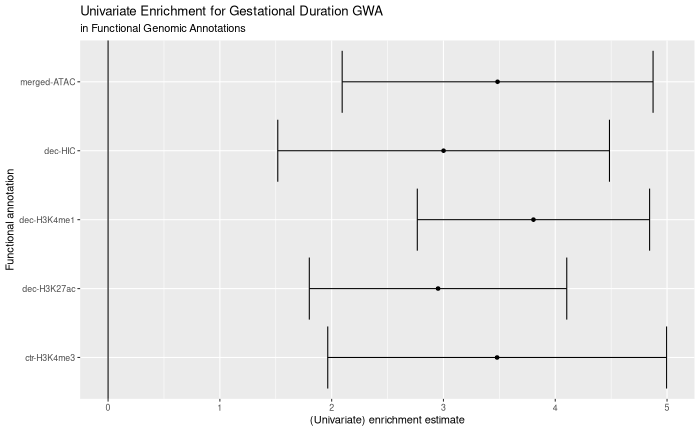
\includegraphics[width=\linewidth]{img/ptb_univ_assoc.png}
    \caption{Univariate enrichment for gestational duration GWAS signal in regulatory maps of decidua-derived stromal cells. TORUS was run on each }\label{fig:univ_assoc}
  \end{subfigure}
    \begin{subfigure}[t]{\textwidth}
    \centering
    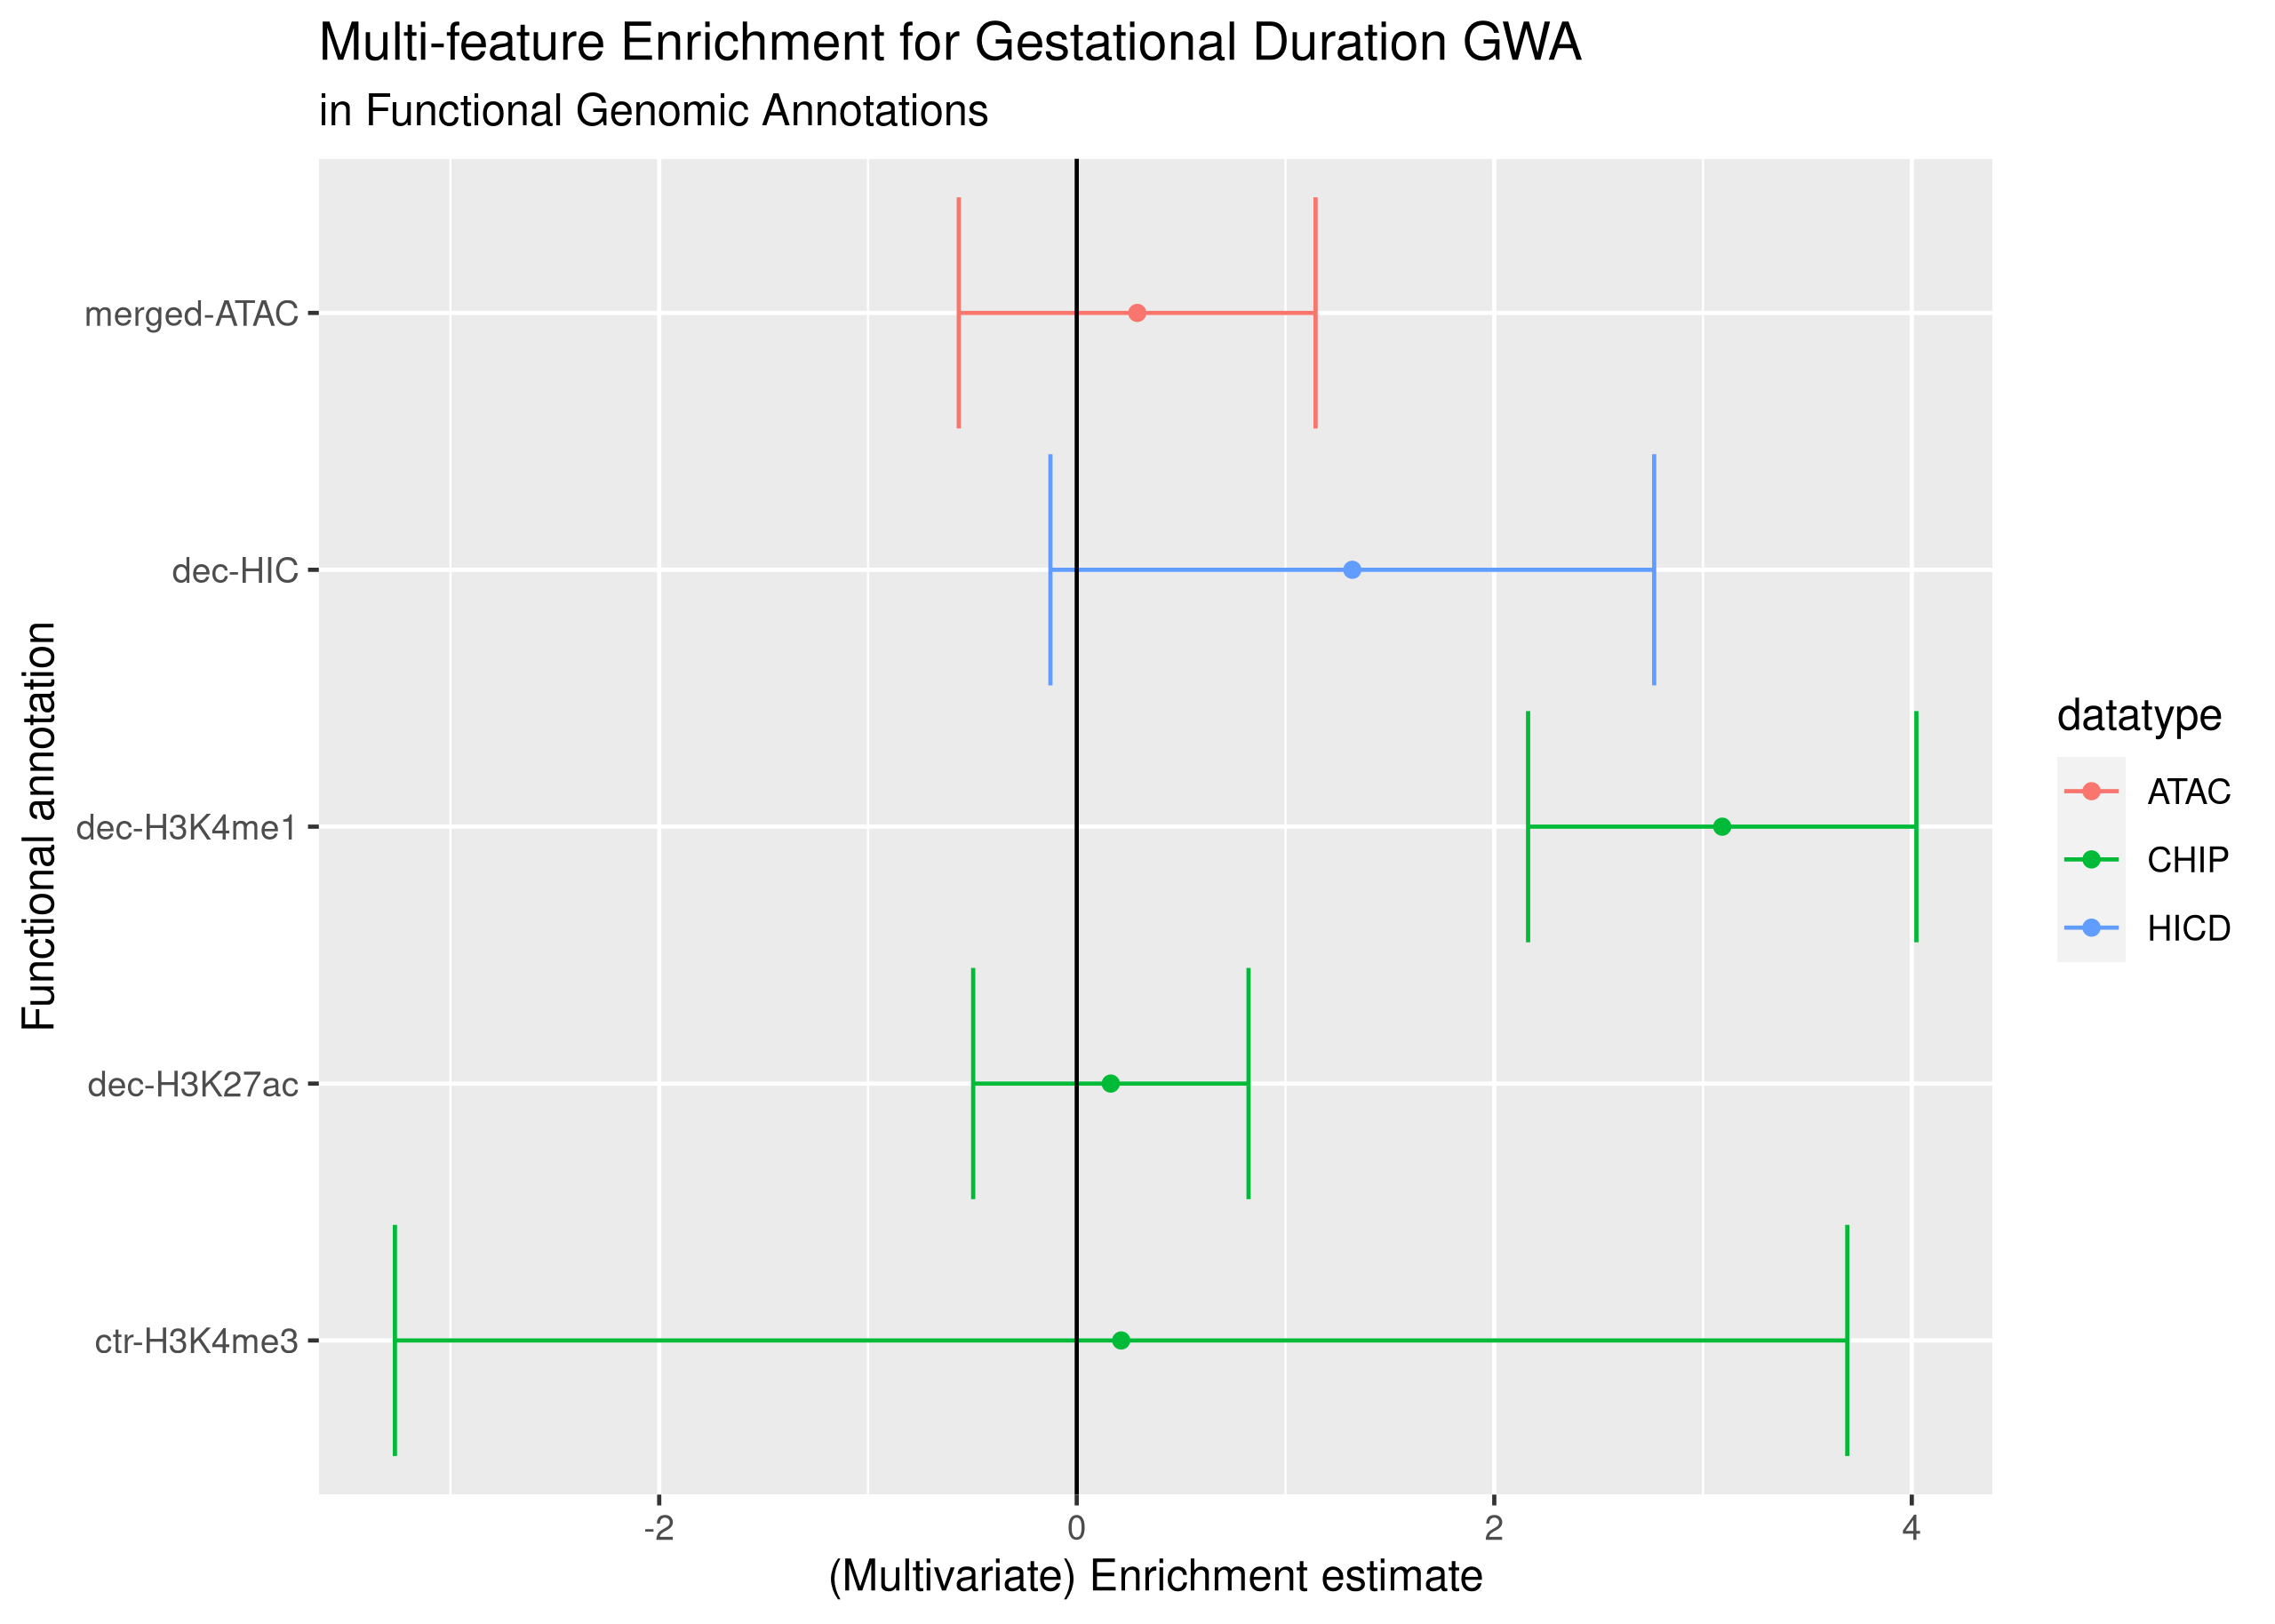
\includegraphics[width=\linewidth]{img/ptb_multiv_assoc.png}
    \caption{Multivariate enrichment for gestational duration GWAS signal}\label{fig:multiv_assoc}
    \end{subfigure}
\end{figure}



\subsection{Functionally informed gene-level fine mapping of gestational duration genes}

We developed a computational procedure to integrate the decidua stromal cell functional maps with genetic map of reproductive traits.
We posited that integrating functional maps in these pregnancy-relevant cells and leveraging statistical methods to fine-map associations
would result in 1) identifying candidate causal variants in each associated locus, 2) linking those variants to their target genes, and
3) discovering additional loci and genes associated with gestational duration. 

We first leveraged the enrichments of DSC annotations to create Bayesian prior probabilities for a variant being causal. Using prior probabilities informed by functional annotations of SNPs could increase the accuracy of fine-mapping, as shown in recent studies (8, 41). We chose H3K27ac, H3K4me1, and pcHi-C interactions from the decidualized cells, and H3K4me3 from untreated cells, and ATAC-seq peaks from any of the cells as functional genomic annotations to create informative priors using TORUS\cite{torus}. To assign a prior to each SNP, TORUS uses genome-wide summary statistics of GWAS and the functional annotations to assess how informative each annotation is in predicting causal variants. SNPs associated with functional annotations are generally assigned higher prior probabilities. Additionally, TORUS computes statistical evidence at the level of genomic blocks, defined as the probability that a block (determined by LD) contains at least one causal SNP. Without including any histone marks or chromatin accessibility annotations, TORUS implicated six autosomal blocks in the genome at FDR < 0.05, including five of the six genome-wide significant autosomal loci identified in the GWAS (p < 5x10-8).
% One locus on chromosome 3 had an FDR = 0.11, and was therefore not identified by TORUS and one locus on chromosome 9 that was not identified in the GWAS was implicated by TORUS (Supplementary File S4).
By including the functional genomic annotations from endometrial stromal cells, the number of high confidence blocks increased to ten, including all six that were significant in the gestational duration GWAS and four that were not significant in the GWAS (Supplementary File S4).  

We next performed computational fine mapping on the top these ten blocks, with the informative priors learned by TORUS, using SuSiE(43). Conceptually, SuSiE is a Bayesian version of the stepwise regression analysis commonly used in GWAS (i.e. conditioning on one variant, and testing if there is any remaining signal in a region). SuSiE accounts for the uncertainty of causal variants in each step, and reports the results in the form of posterior including probabilities (PIPs). The PIP of a variant ranges from 0 to 1, with 1 indicating full confidence that the SNP is a causal variant. If a region contains a single causal variant, the PIPs of all SNPs in the region should approximately sum to 1.  

Including the priors defined by TORUS using DSC functional annotations significantly improved fine-mapping (Figure 5A, Supplementary Table S3 and Supplementary File S5. For example, only one SNP reached PIP > 0.3 across all 10 blocks using the default setting under SuSiE (uniform prior, treating all SNPs in a block equally). This reflects the general uncertainty of pinpointing causal variants due to LD: e.g., a strong GWAS SNP in close LD with 9 other SNPs would have PIP about 0.1. By using the annotation-informed priors, 8 SNPs in six different blocks reached PIP > 0.3 (Figure 5A). In some blocks, we were able to fine-map a single high-confidence SNP, e.g. the FOXL2 locus on chromosome 3, while in other blocks, we had considerable uncertainty of the causal variants, as shown by large credible sets, i.e. the minimum set of SNPs to include the causal SNP with 95\% probability (Figure 5B). Table 1 summarizes the most probable causal variants in eight blocks (fine-mapping in the remaining two blocks produced large credible sets with no high-PIP SNPs) as well as their likely target genes based on promoter assignment or chromatin interactions from pcHi-C. We note that our results of the WNT4 locus identified rs3820282 as the likely causal variant. This is consistent with our previous results demonstrating experimentally that the T allele of this SNP disrupts the binding of estrogen receptor 1 (ESR1)(5). This SNP was among the 3 most likely SNPs in our fine-mapping study, with a PIP of 0.27 (Table 1). 



We highlight the results from two regions. In the first, two adjacent SNPs (311 bp apart), rs13141656 and rs7663453, on chromosome 4q34 did not reach genome-wide significance in the GWAS (p = 3.9 ×10-7 and 4.5 ×10-7, respectively). After using functional annotations in decidua-derived stromal cells, the block containing these SNPs was highly significant (TORUS q-value = 0.02), suggesting the presence of at least one causal variant in this block. The two SNPs together explained most of the PIP signal in the block (PIP 0.38 and 0.33, respectively, Table 1). The two SNPs are located in a region of open chromatin in endometrial stromal cells, with enhancer activity marked by both H3K27ac and H3K4me1 (Figure 5C). Only 9 of the 129 tissues from the Epigenome Roadmap(11) also had H3K27ac, H3K4me1 or H3K4me3 peaks spanning the rs13141656 locus and only 2 spanning the rs7663453 locus. In addition, this putative enhancer is bound by multiple transcription factors, including GATA2, FOXO1, NR2F2 and PGR, based on ChIP-seq data. The only physical interaction of this enhancer in the pcHi-C data in decidualized stromal cells is with the promoter of the HAND2 gene, located 277 kb away (Figure 5C). Summing over the PIPs of all SNPs whose nearby sequences interact with HAND2 via chromatin looping gives an even higher probability, 0.89, suggesting that HAND2 is very likely to be the causal gene in this region (Supplementary Table S4). HAND2 is an important transcription factor that mediates the effect of progesterone on uterine epithelium(45). Thus, in this example we identified a novel locus, the likely causal variant(s), the enhancers they act on, and an outstanding candidate gene for gestational duration and PTB.  

The second example focuses on the locus showing a strong GWAS association with gestational duration on chromosome 3q21. The lead SNP, rs144609957 (GWAS p = 4 ×10-13), is located upstream of the EEFSEC (Eukaryotic Elongation factor, Selenocysteine-TRNA Specific) gene. There is considerable uncertainty of the causal variants in this region, with 50 SNPs in the credible set and the lead SNP explaining only a small fraction of signal (PIP = 0.02). Among all 12 SNPs with PIP > 0.01, 11 have functional annotations, most commonly H3K4me1 and pcHi-C interactions. Interestingly, for nine SNPs (first 3 shown in Table 1), the sequences in which they are located physically interact with the promoter of GATA2 in the pcHi-C data, but not with any other promoters in the region (Supplementary Figure S3). The PIPs of all SNPs in the genomic regions that likely target GATA2 through chromatin looping sum to 0.68 (Supplementary Table S5). Thus, despite uncertainty of causal variants in this region, our results implicate GATA2 as a candidate causal gene in endometrial stromal cells. GATA2 is a master regulator of embryonic development and differentiation of tissue-forming stem cells(46). As support for the possible role of GATA2 in pregnancy, GATA2 deficient mice show defects in embryo implantation and endometrial decidualization(34), making this another excellent candidate causal gene for gestational duration and PTB. 


\begin{figure}
  \centering
    \begin{subfigure}[t]{\textwidth}
    \centering
    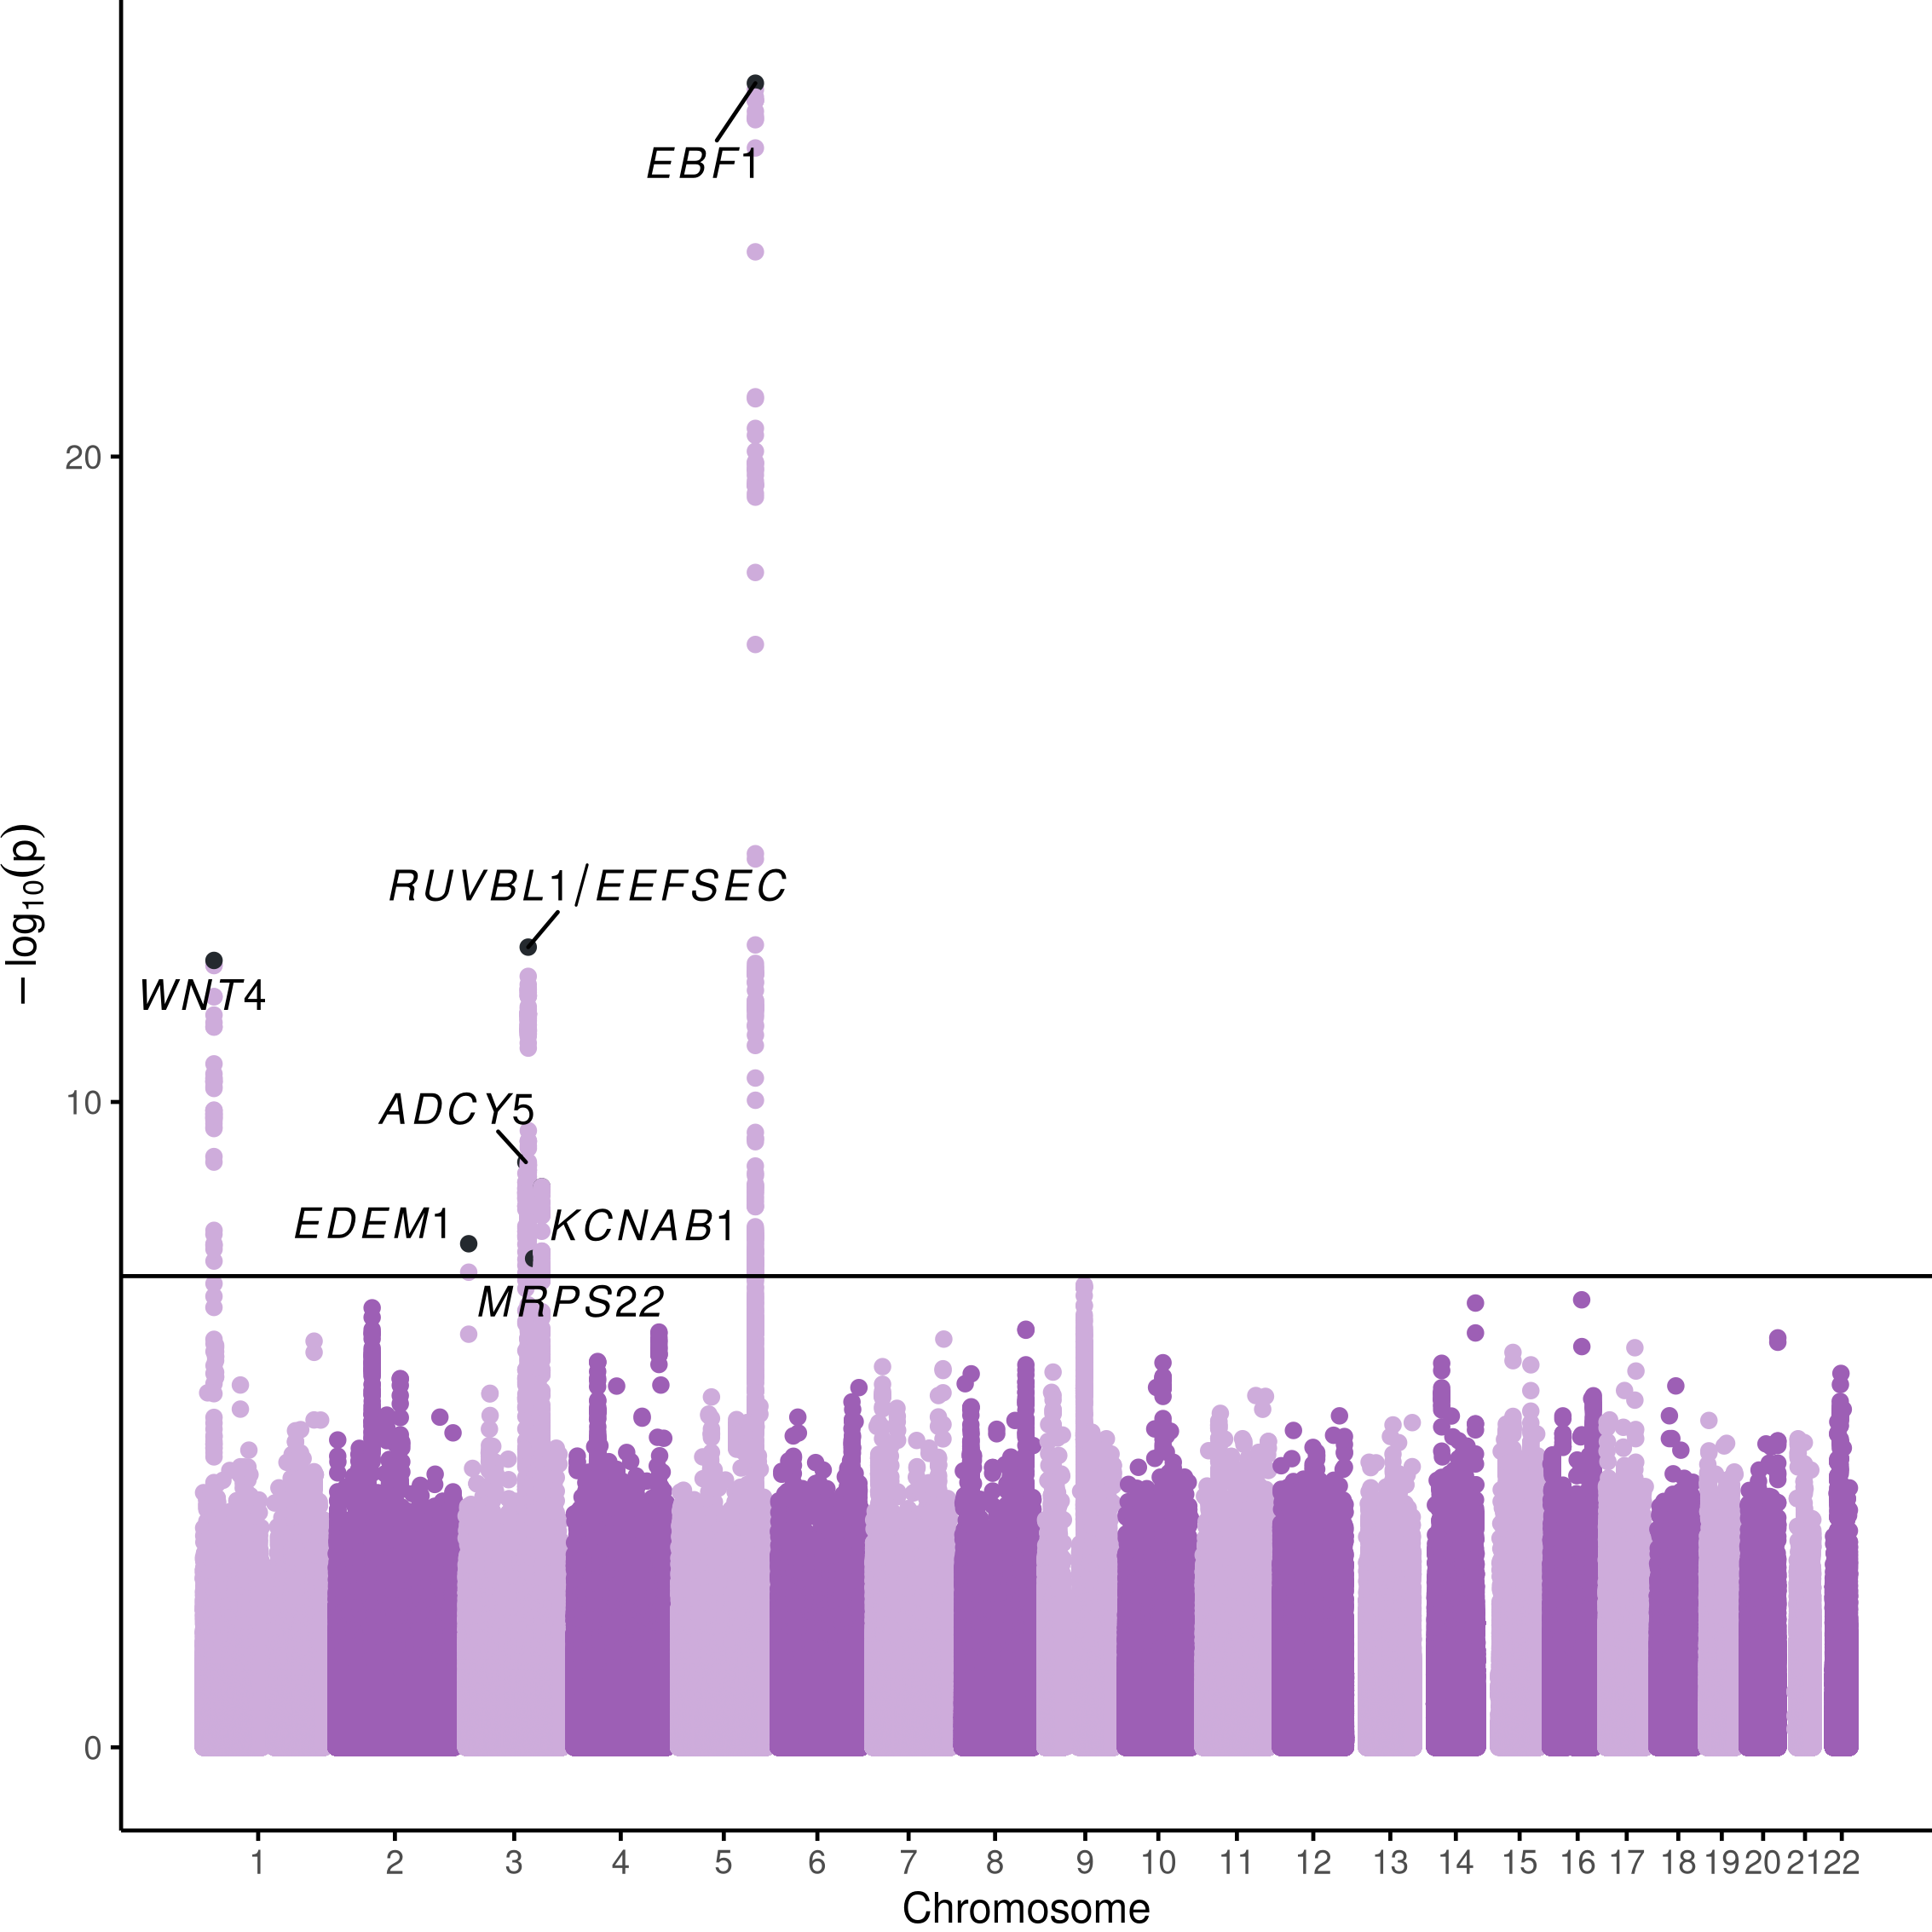
\includegraphics[width=\linewidth]{img/FigureS_Manhattan_plot.png}
    \caption{Manhattan plot of a GWAS for gestational duration GWAS. The horizontal black line denotes the threshold for genome-wide significance ($p < 5 \times 10^{-8}$). For the 6 independent genome-wide significant loci, the most significant p-value is highlighted in black, and labeled with the nearest gene(s).}\label{fig:manhattan}
  \end{subfigure}
\end{figure}

\begin{figure}
  \centering
  \begin{subfigure}[t]{\textwidth}
    \centering
    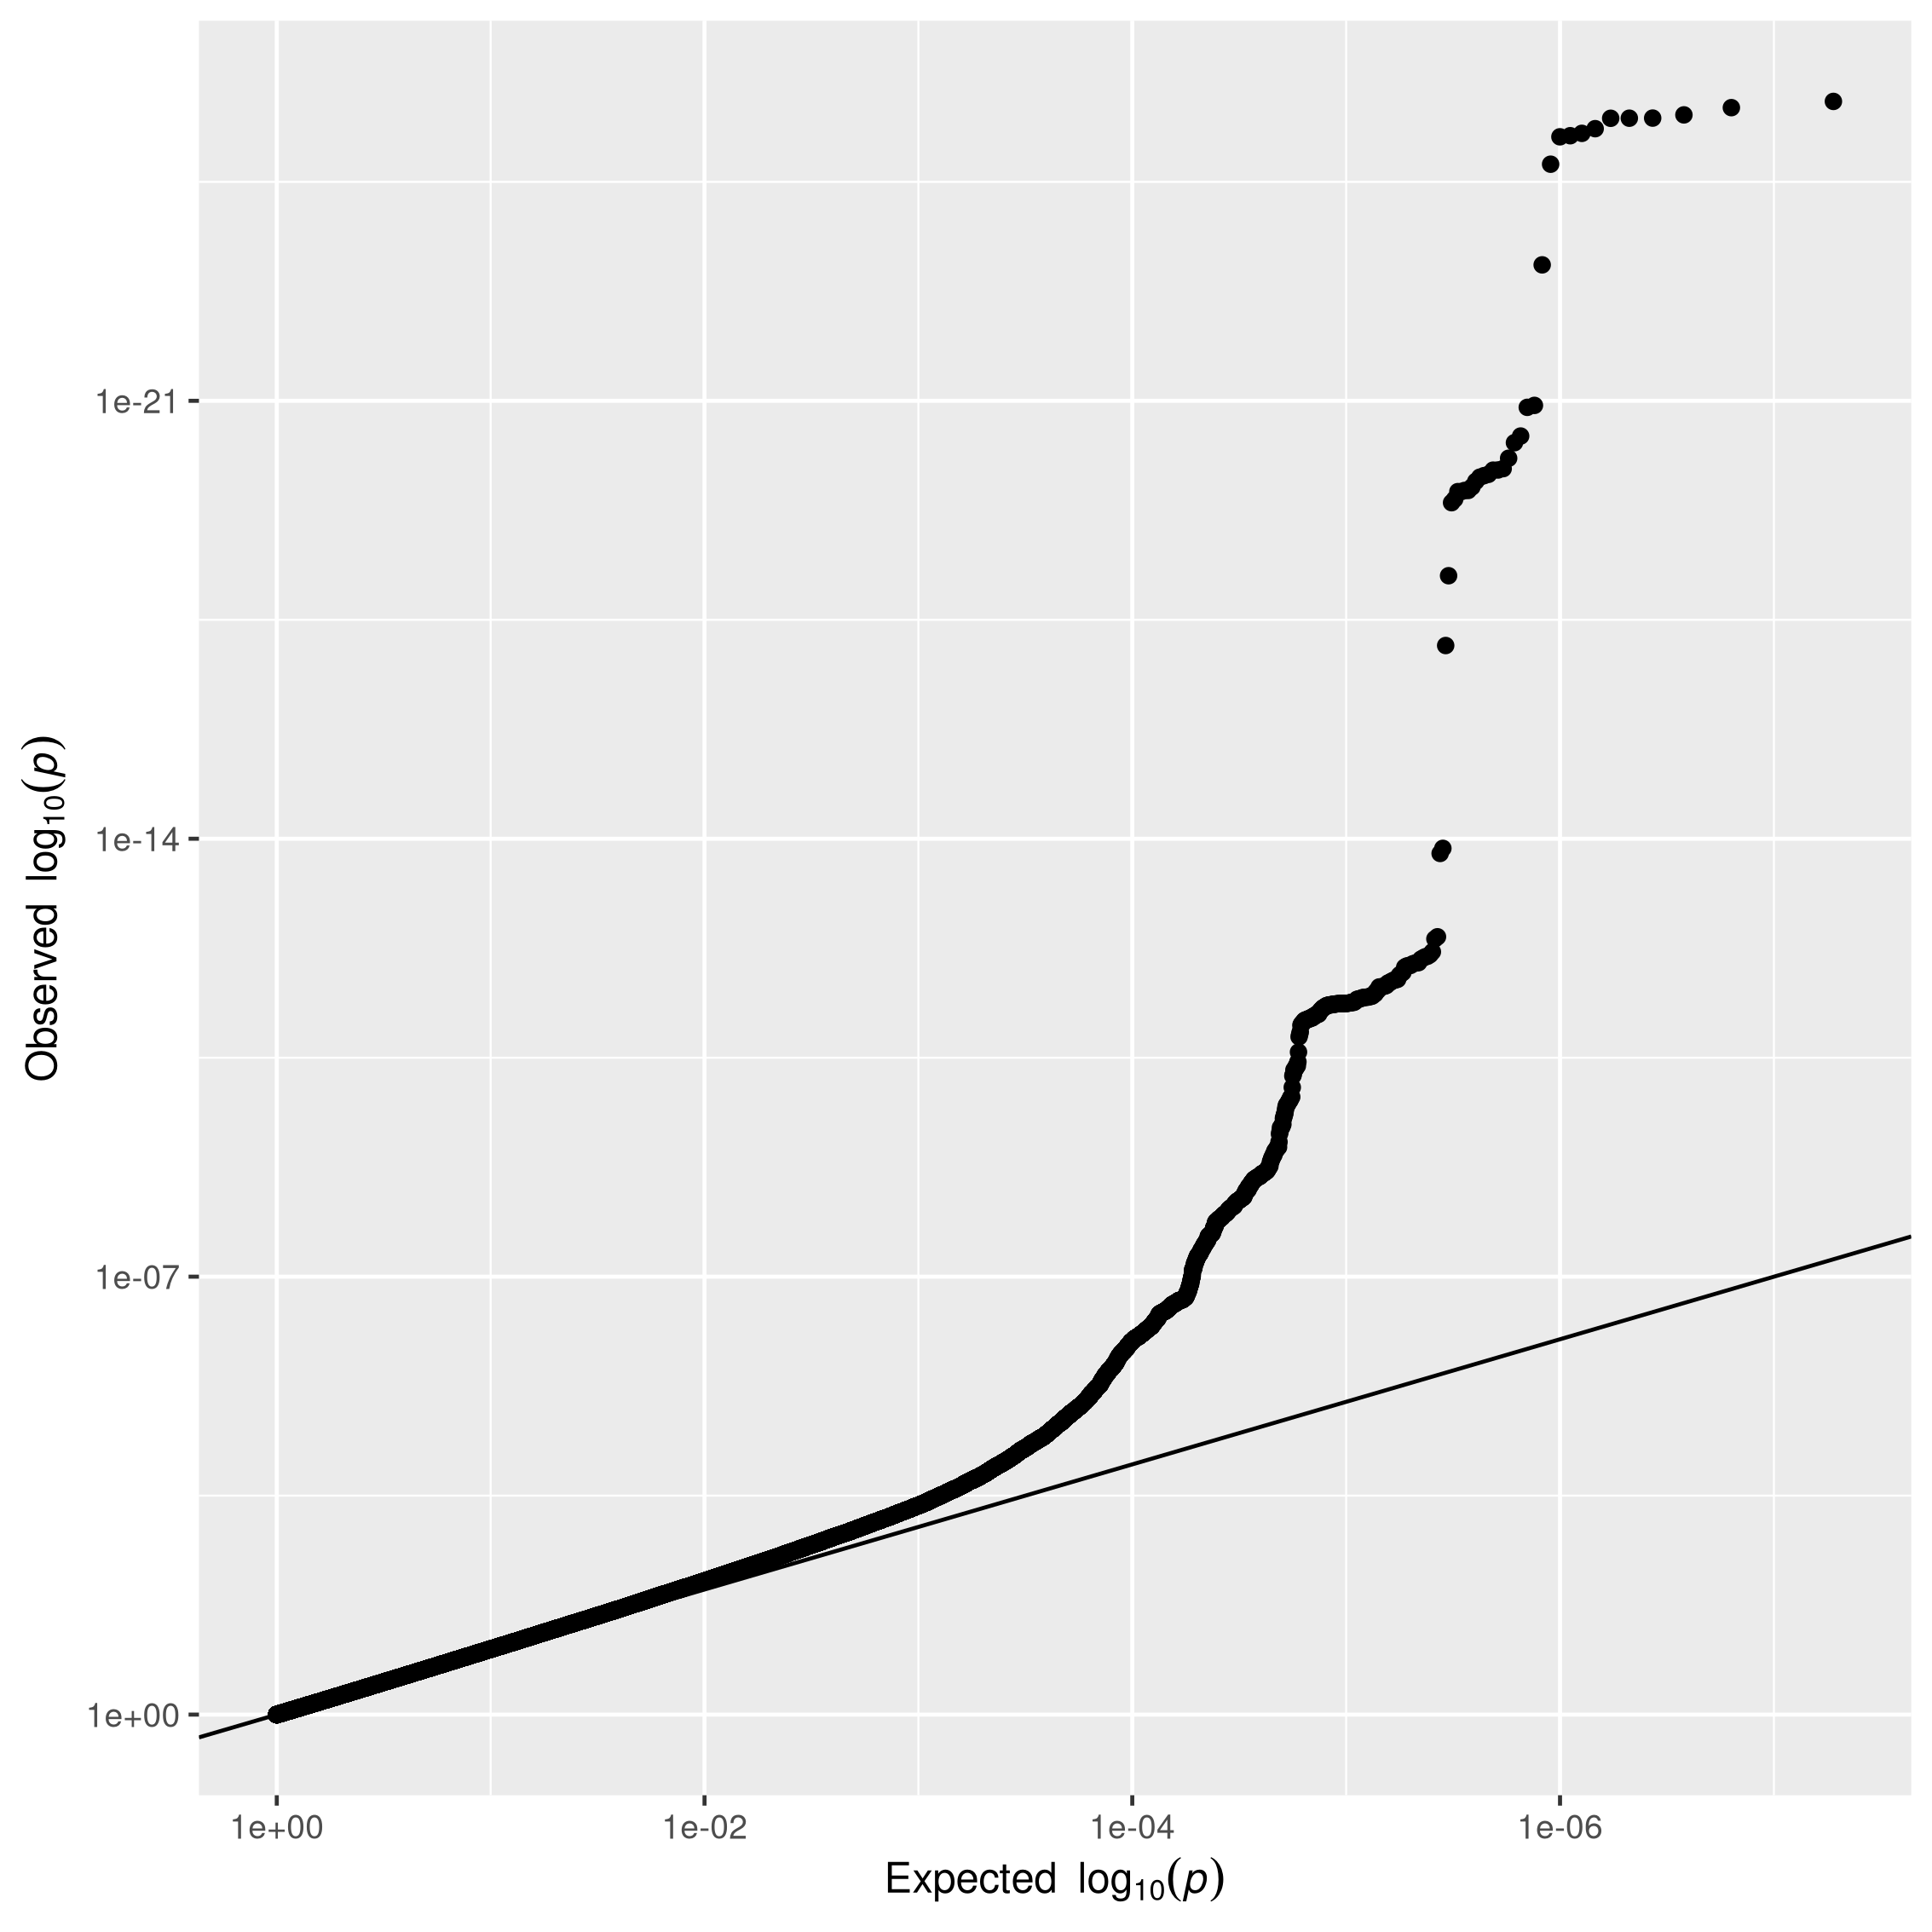
\includegraphics[width=\linewidth]{img/FigureS_qq_plot.png}
    \caption{QQ plot of p-values from the GWAS of gestational duration.}\label{fig:qqplot}
  \end{subfigure}
\end{figure}


\begin{figure}
  \centering
  \begin{subfigure}[t]{\textwidth}
    \centering
    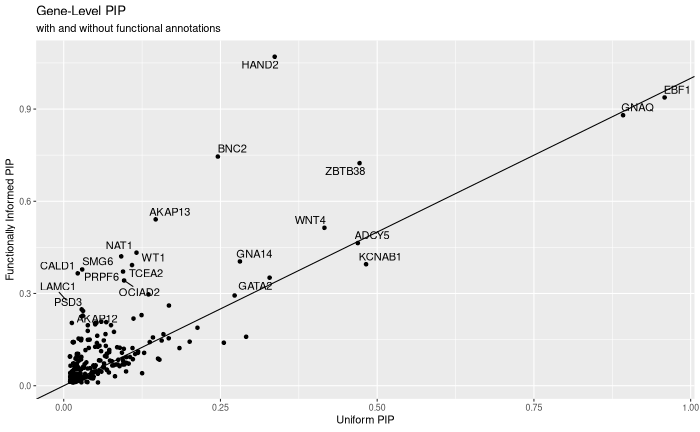
\includegraphics[width=\linewidth]{img/null-gene-gene-comp.png}
    \caption{Gene-level PIPs under the functionally informed model as compared to the uniform model.  The same variant-gene assignment was used for both models.  Genes above the black diagonal line have a higher gene-level PIP under the functionally-informed model compared to the uniform model.  }\label{fig:univ_assoc}
  \end{subfigure}
    \begin{subfigure}[t]{\textwidth}
    \centering
    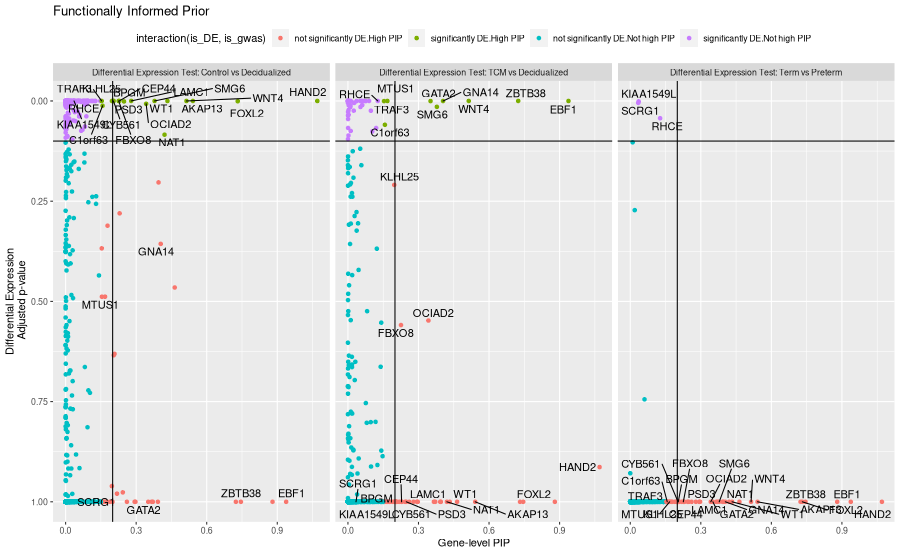
\includegraphics[width=\linewidth]{img/de-gwas-comp.png}
    \caption{Differential expression adjusted $p$-value for each of three differential expression tests: control vs decidualized, decidualized vs TCM-treated, and term vs preterm, along with the gene-level PIP for the corresponding gene for the 686 genes in the 33 genomic regions most likely to contain a gestational duration GWAS variant.  The vertical and horizontal lines indicated thresholds that were used to test for the enrichment of high PIP genes for differentially expressed genes. High PIP genes were significantly enriched for both differential control vs decidualized genes ($p=0.0264$), and for differential decidualized vs TCM-treated genes ($p=0.0344$), by fisher's exact test.}\label{fig:multiv_assoc}
    \end{subfigure}
\end{figure}




\section{Discussion}\label{sec:org53f1196}

 The lack of complete independence between these marks makes it difficult to delineate their individual effects but nonetheless highlights the importance of enhancers and of gene regulation in endometrial stromal cells in modulating the effects of GWAS variants on gestational duration. This is consistent with both the known tissue-specific roles of enhancers and the observation that over 90\% of GWAS loci reside outside of the coding portion of the genome and are enriched in regions of open chromatin and enhancers(12, 40). 

    Integrating transcriptional and chromatin annotations of gene regulation from MSCs and DSCs improved our ability to discover novel GWAS loci and identify likely causal SNPs and genes associated with gestational duration. We illustrate how our integrated platform identified a novel causal locus and candidate gene (HAND2) associated with gestational duration, as well as refined the annotation of loci that had been previously identified. Our data suggest that in endometrial stromal cells GATA2 is likely the target gene of enhancers harboring SNPs associated with gestational duration. This does not exclude the possibility that the nearest gene to the associated SNPs, EEFSEC, may be a target gene in other cell types.  

    Both of these examples highlight transcription factors that are essential for endometrial development or decidualization. The fact that neither GATA2 nor HAND2 were identified as potential candidate genes in previous GWASs of gestational duration or PTB supports our approach and the importance of using functional annotations from cell types relevant to pregnancy to fine map and identify candidate genes for the pregnancy-related traits. Overall, the integrated analyses performed in this study resulted in the identification of both novel GWAS loci and novel candidate genes for gestational duration, as well as maps of the regulatory architecture of these cells and their response to decidualization. 

    However, there are some limitations. Our results are based on only 3 individuals, which may not be enough to fully capture the regulatory landscape of endometrial stromal cells. In addition, the 3 individuals were African American and the GWAS results were obtained from Caucasians individuals and therefore, it is possible that the GWAS results do not match functional annotations in a different population, which could lead to erroneous conclusions. Another limitation is the fact that we focused on only one cell type, albeit one that plays a central role in pregnancy, and only one exposure (hormonal induction of decidualization) and only for 48 h. Different exposures could lead to different results. Future studies that include fetal cells from the placenta and uterine or cervical myometrial cells could reveal additional processes that contribute to gestational duration and PTB, such as those related to fetal signaling and the regulation of labor, respectively. Inclusion of additional exposures, such as trophoblast conditioned media(49), may further reveal processes that are pregnancy-specific. Second, to maximize power we focused on a GWAS of gestational duration and not PTB per se. While previous GWAS have shown that all PTB loci were among the gestational age loci(5), we realize that some of the loci that we identified could be related to normal variation in gestational duration and not specifically to PTB. Nonetheless, our findings contribute to our understanding of potential mechanisms underlying the timing of human gestation, about which we still know little. Lastly, although our ChIP-seq results revealed an association between GATA2 binding and decidualization, confirming the role of this transcription factor in decidual cell biology(50, 51), and studies in murines support its role in endometrial processes(34), we do not yet have direct evidence showing that perturbations in the expression of GATA2, or any of the other target genes identified, influence the timing of parturition in humans. Future studies will be needed to directly implicate the expression of these genes in gestational duration or PTB. Our study highlights the importance of generating functional annotations in pregnancy-relevant cell types to inform GWASs of pregnancy-associated conditions. Our results suggest that the expression of two transcription factors, GATA2 and HAND2, in endometrial stromal cells may regulate transcriptional programs that influence the timing of parturition in humans, which could lead to the identification of biomarkers of or therapeutic targets for PTB




% \subsubsection{A comment on distance to the nearest gene}


% ``Nearest gene'' is a an important benchmark when considering alternative methods for associating a variant with a gene\cite{fine2019benchmarker}.  In measuring the distance between a particular variant and surrounding genes, uncertainty may arise as as consequence of the ambiguity around the term ''gene''.



% Without attempting to define what a ge  to which gene is Without diverting iThere are several scenarios where the gene that is closest to a given variant depends on the definition of ``clo  distance from a variant to a gene can be calculated in One common approach for measuring the distance between variants to genes is to take the distance between        for evaluating the effectiveness of a snp-gene mapping distance to TSS is relevant for enhancer promoter looping conditioned on transcription initiation, what's the relevance of distance to TSS?
% Introns are worthy of special consideration, as they constitute approximately 25 percent of the human genome, and as they are, by definition, close to while distinct from the coding regions of the genome.    

% There are many possible mechanisms by which an intronic variant might act through a (protein-coding) gene to drive GWAS signal.
% Disrupting an enhancer is one such mechanism, but there are many additional mechanisms that involve altering transcription downstream of initiation.   (e.g APA, erroneous splice site, promoting RNA degradation, stalling elongation) and none of those really relate to distance to TSS.    For "early" introns/small genes the distance to TSS won't be much different from distance to nearest exon so it won't really matter, and for "late" exons in big genes the distance to the next downstream gene's TSS could be much closer to the variant.   Even if enhancers are very likely to target the nearest TSS (rather than nearest gene), you are more or less discounting all other causal mechanisms when you define "distance to gene" to be distance to TSS.
% 1:23 by "most of the mechanisms" I don't mean they're collectively more likely, I just mean there are many ways to disrupt a gene after transcription. lastly, the SNPs we're trying to assign to genes based on distance are going to (hopefully) be depleted for enhancers because of the HiC mapping step. Even if the non-enhancer mechanisms are relatively rare, they're more likely in our case.

% Chapter 04
\chapter{Conclusion}
\label{conclusion}
I now conclude my dissertation


% Format a LaTeX bibliography
\makebibliography

% Figures and tables, if you decide to leave them to the end
%\input{figure}
%\input{table}

\end{document}
